\chapter{Búsqueda de SUSY con fotones y Higgs en el estado final con producción fuerte}\label{cap:analysis}
% \addcontentsline{toc}{chapter}{Búsqueda de SUSY con fotones y Higgs en el estado final}
\chaptermark{Búsqueda de SUSY con fotones y Higgs en el estado final con producción fuerte}


% Rescrito de Tesis lic
% El análisis para el cual está orientada esta Tesis consiste en la búsqueda de Supersimetría en eventos con un fotón aislado muy energético, jets y gran cantidad de energía faltante en estado final \cite{Alonso:2147473,ATLAS:2016fks,Collaboration:2198651}. La estrategia general de la búsqueda consiste en el conteo del número de eventos observado en exceso sobre el SM en una cierta región del espacio de observables rica en eventos de la señal considerada.


El trabajo realizado en esta Tesis se centra en la búsqueda de Supersimetría en eventos con al menos un fotón energético y aislado, jets y gran cantidad de energía faltante en el estado final. La estrategia general de la búsqueda consiste en el conteo del número de eventos observados, y su comparación con las predicciones del SM, en regiones del espacio de observables ricas en eventos de la señal, siguiendo los métodos descriptos en el Capítulo \ref{cap:statistical}. El objetivo es poder discriminar en los datos observados, aquellos que podrían ser producto de un proceso supersimétrico (señal), de aquellos provenientes de procesos del SM (fondo).


\section{Muestras de señal a partir de simulaciones Monte Carlo}\label{sec:signal_samples}

El modelo supersimétrico que motiva a la presente búsqueda consiste en un modelo GGM, y por lo tanto el gravitino es la LSP, cuya masa es del orden de unos pocos eV. La NLSP, en este caso, es el neutralino más liviano, que consiste en un estado de gauge mezcla de bino y higgsino, lo que le permite acoplar a fotones, bosones $Z$ y bosones de Higgs.
Análisis anteriores se centraron en los casos donde el neutralino acopla solamente a fotones y bosones $Z$ \cite{Alonso:2147473, tesis_joaco, Collaboration:2198651, tesis_tony}, o solamente a fotones \cite{Jinnouchi:2233741}. El trabajo realizado en esta Tesis se centra en el caso fenomenológico en el cual el neutralino más liviano decae en proporciones iguales a $\gamma+\gravino$ y a $h+\gravino$. Esto último es posible si el parámetro $\mu$ toma valores negativos, favoreciendo así el decaimiento al Higgs, y reduciendo notablemente 
% \solved{puse reduce porque no lo suprime del todo} ok
el decaimiento al bosón $Z$.
% , en cuyo caso ya fue previamente estudiado por otros análisis \cite{tesis_fran, tesis_joaco}. 
Para la producción de partículas supersimétricas a partir de la colisión $pp$ se considera inicialmente la producción de gluinos. La parte del análisis que comprende la producción electrodébil se describe en el Capítulo \ref{cap:analysis_EWK}. Dichos gluinos decaen subsecuentemente en partículas más livianas, hasta llegar a las NLSP y luego a la LSP.
Como el gluino tiene carga de color y la NSLP no, el decaimiento esta intermediado por squarks virtuales, produciendo jets adicionales.
Cadenas de decaimiento típicas de este modelo se pueden observar en la Figura \ref{fig:phb_feyn}.

\begin{figure}
  \centering
  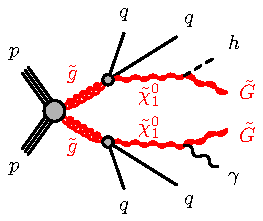
\includegraphics[width=0.45\textwidth]{images/analysis/gogo-qqqqbbphGG-h_short.pdf}
  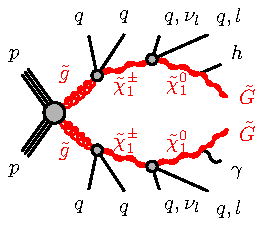
\includegraphics[width=0.45\textwidth]{images/analysis/gogo-qqqqbbphGG-h_long.pdf}
  \caption{Producción fuerte de gluinos con posibles decaimientos en el estado final estudiado. A la izquierda se observa un decaimiento directo del \gluino a \ninoone, mientras que a la derecha se observa un decaimiento del \gluino mediante \chinoonepm (el cual también podría ser mediante \ninotwo).}
  \label{fig:phb_feyn}
\end{figure}

En la Sección \ref{sec:susy} se describe al MSSM junto con la gran cantidad de parámetros que lo caracterizan. 
% \solved{Reescrito}
% Cuando se desea generar muestras para un modelo, se debe elegir valores para esos parámetros que a priori son arbitrarios, y cuya única posible elección son los distintos objetivos del análisis. A su vez, se busca que al seleccionar valores para esos parámetros, tener el compromiso de no ser muy específicos con esos valores, ya que de esa forma el análisis terminaría siendo demasiado dedicado a un modelo particular. Ni tampoco muy arbitrarios, ya que se busca seguir manteniendo de alguna forma la fenomenología del mismo. Lo que se hace entonces es reducir los parámetros que caracterizan al modelo a unos pocos, y utilizar distintos programas de calculo que se encargan a partir de ellos generar tanto el espectro completo de masas, como los distintos posibles decaimientos de cada partícula.
Al realizar el estudio experimental, motivado por un dado modelo, se debe acotar la cantidad de parámetros y sus posibles valores, maximizando de esta forma la producción del estado final buscado. En este contexto, si bien se realizan búsquedas motivadas por un dado modelo, al seleccionar y definir las regiones de señal, se posibilita que el espacio de parámetros seleccionado pueda ser también inclusivo a otros potenciales modelos de nueva física. 

El parámetro característico de este modelo es $\mu$, el cual toma valores negativos para habilitar el decaimiento del \ninoone a Higgs. A su vez, se busca suprimir el decaimiento al bosón $Z$, y que el decaimiento a fotones sea igual de probable que el decaimiento al Higgs. Como se desea tener este comportamiento de forma uniforme para todas las masas de \ninoone estudiadas, es necesario encontrar un valor óptimo de $M_1$ que satisfaga dichas condiciones. Se encuentra que mediante la relación $M_1 \sim |\mu|$,
% \solved{Acá había encontrado una fórmula mediante un fit para M(mu), pero no se si es importante} Mejor no ponerlo...
es posible reducir el decaimiento al bosón $Z$ hasta casi un 10\%, dejando a los otros dos decaimientos aproximadamente en un 45\% para todas las masas de \ninoone, como muestra la Figura \ref{fig:n1_br}. 
% Como el modelo es un GGM, se fijó la masa del \gravino en $1$ eV 
% \solved{esto no es tan así, la masa variaba de acuerdo al mu, lo deberia poner?}. Corregido

\begin{figure}
  \centering
  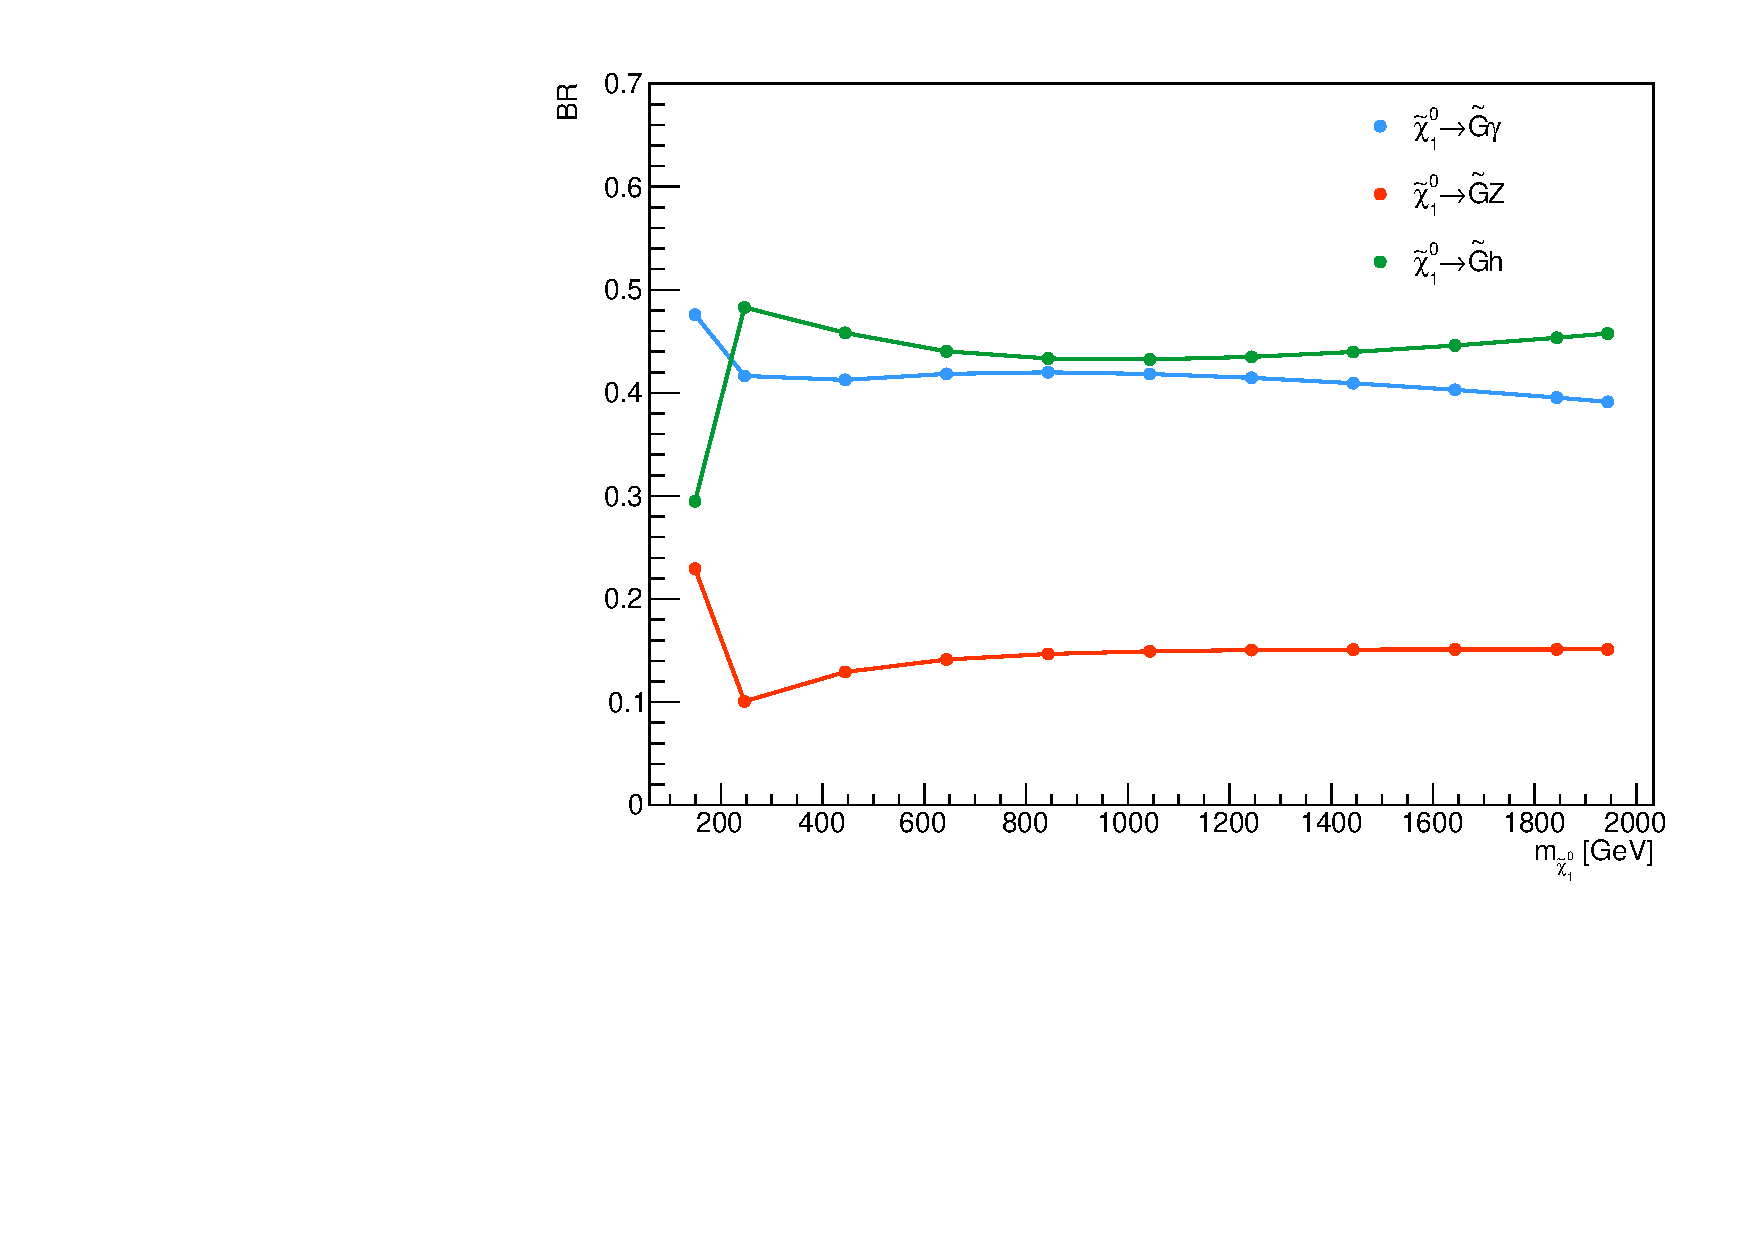
\includegraphics[width=0.6\textwidth]{images/analysis/phb_n1_br.pdf}
  \caption{Fracción de decaimiento (BR) del \ninoone en función de la masa del mismo.}
  \label{fig:n1_br}
\end{figure}

Las muestras se generan considerando la producción de gluinos a partir de la colisión $pp$, con 0, 1 o 2 jets adicionales de ISR. Para esto, se considera al gluino como la única partícula supersimétrica de color relevante, por lo que las masas de los squarks se fijan a \magn{5}{TeV}, evitando así toda posible producción \textit{on-shell} de los mismos (en lo que se denomina desacoplamiento). Los gluinos producidos en la colisión, decaen a un par de quark-antiquark más algún gaugino como se muestra en la Ecuación \ref{eq:gluino_dec}. Esto ocurre mediante squarks virtuales los cuales son completamente degenerados, pudiendo ser cualquiera de los 12 estados de sabor/quiralidad.
Al igual que con los squarks, se elige la masa de los sleptons igual a \magn{5}{TeV}, evitando así su producción.
% , la cual es estudiada por otros análisis \solved{citar analisis}. % na
Además, se anulan todos los términos de acoplamiento trilineal, y se fija $M_2=3\,\tev$ y $\tan{\beta}=1.5$, observándose reducida sensibilidad del análisis a variaciones de dichos parámetros. Se emplea el bosón de Higgs observado por las colaboraciones ATLAS y CMS \cite{higgs_mass}, con una masa de $m_h=125\,\gev$, y sus decaimientos ocurren de acuerdo a las predicciones del SM, 
% \solved{es asi?} Si, ponele...
donde el predominante es a dos $b$-jets con un {$\smallsim$}58\% de probabilidad de ocurrencia.
% \solved{Cual mismo?} 
% Adicionalmente se pone al mismo en el régimen de desacoplamiento con $m_A = 2\ \tev$. 
Adicionalmente, se colocan a los estados de masas de los dobletes de Higgs en el régimen de desacoplamiento con una masa de \magn{2}{TeV}.
Se fija la vida media del \ninoone, $c\tau_{\text{NLSP}}<0.1$ mm, de tal forma que decaiga rápidamente para que su vértice no esté considerablemente desplazado del punto de colisión. 
La masa del \gravino, la LSP impuesta por los modelos GGM, se fija del orden de \magn{1}{eV}.
La relación entre los parámetros $M_1$, $M_2$ y $\mu$ determina la masa de los gauginos, y genera que los tres primeros neutralinos estén levemente degenerados junto con el primer chargino, teniendo una masa similar a $|\mu|$, mientras que el \ninofour y el \chinotwopm quedan completamente desacoplados. Los posibles decaimientos del \ninotwo son principalmente a \ninoone junto con un par de quarks, leptones o neutrinos. Los del \ninothree son principalmente a \ninoone junto con un fotón. El \chinoonepm decae principalmente a \ninoone junto con un par de quarks o un par leptón-neutrino. Finalmente se anularon los decaimientos directos del \gluino, \ninotwo, \ninothree y \chinoonepm. Como ejemplo, se muestra en la Figura \ref{fig:mass_spec} un espectro de masas para uno de los puntos de señal con $(M_3, \mu) = (2000\,\gev, -1050\,\gev)$. En la Figura \ref{fig:gluino_decays} se observa la fracción de los posibles decaimiento del \gluino con una masa de \magn{2000}{GeV} en función de la masa del \ninoone. 


\begin{figure}
  \centering
  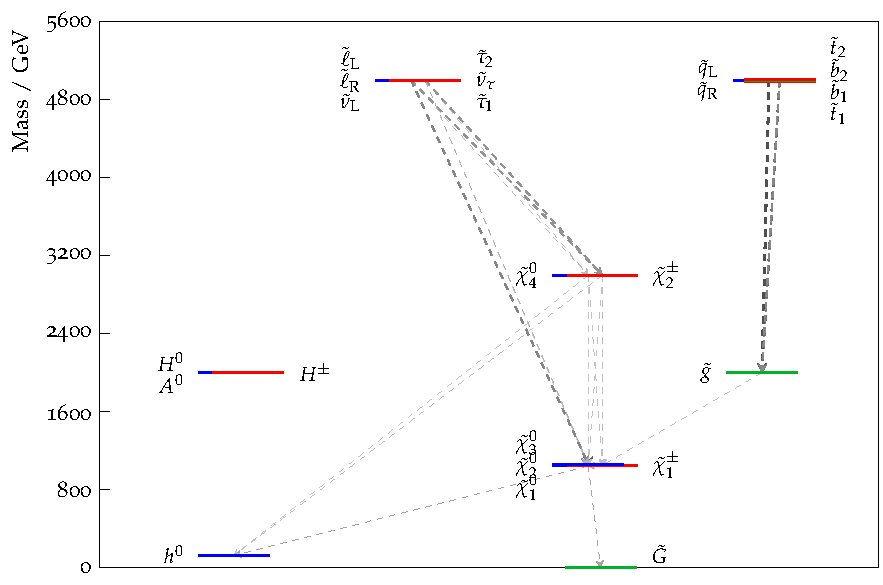
\includegraphics[width=0.6\textwidth]{images/analysis/phb_mass_spectrum.pdf}
  \caption{Espectro de masas de las partículas supersimétricas para el punto de señal con $(M_3, \mu) = (2000\,\gev, -1050\,\gev)$. En gris se muestran algunos de los posibles decaimientos de dichas partículas.}
  \label{fig:mass_spec}
\end{figure}

\begin{figure}
  \centering
  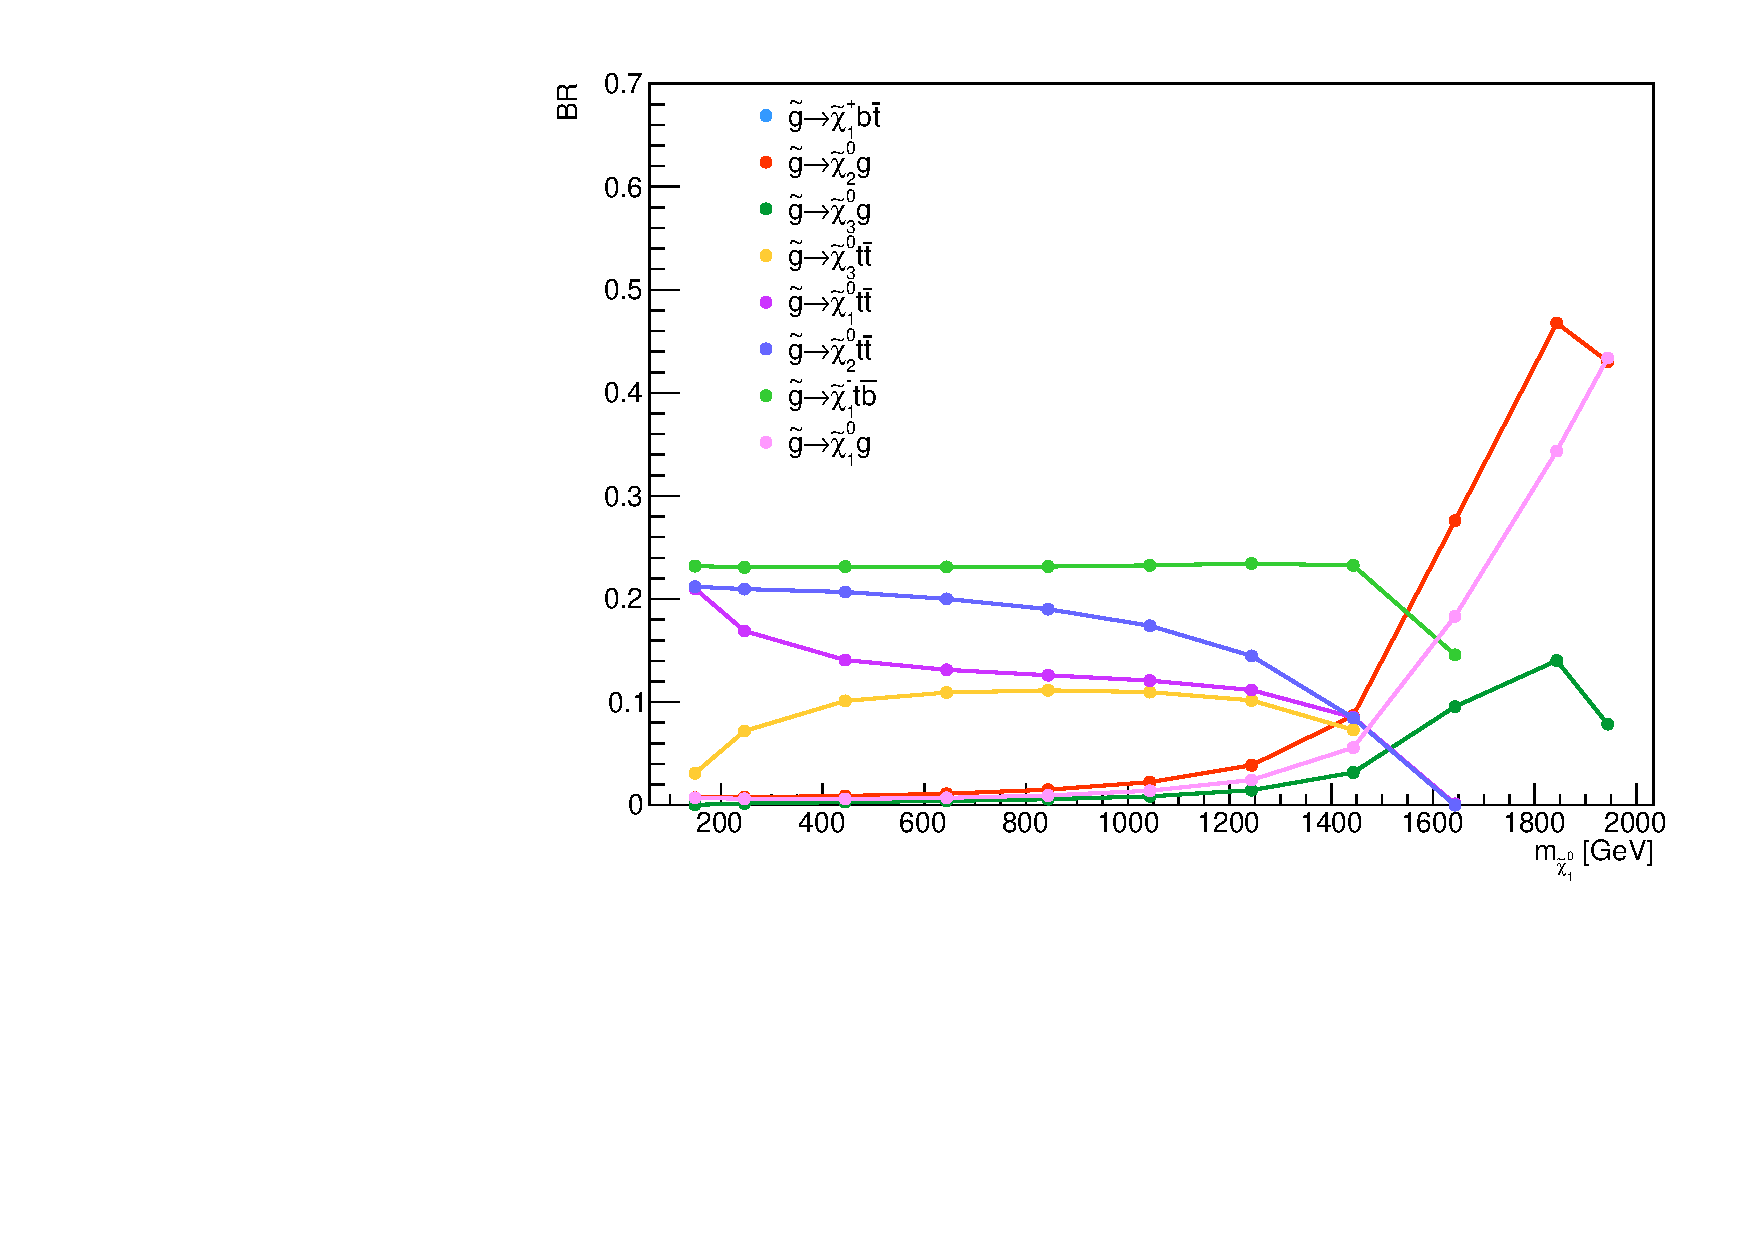
\includegraphics[width=0.6\textwidth]{images/analysis/phb_go_br.pdf}
  \caption{Fracción de decaimiento del \gluino con una masa de \magn{2000}{GeV} en función de la masa del \ninoone.}
  \label{fig:gluino_decays}
\end{figure}


% \solved{mencionar decaimientos masas de los demas neutralnos y charginos} done

Debido a que son varios los análisis que estudian la producción de gluinos, la colaboración ATLAS genera archivos comunes a todos los análisis donde ya tiene almacenada la información de varios eventos de producción de gluinos. Estos archivos se denominan Les Houches Event (LHE) \cite{Alwall:2006yp}, que estandarizan esta etapa de simulación, y solo resta generar las cadenas de decaimiento de los gluinos de acuerdo a los distintos modelos estudiados. En el presente análisis se omiten las correcciones radiativas así la masa de los gluinos coincide con el parámetro $M_3$.
% \solved{reescrito}
% , pudiendo así coincidir con los archivos LHE que están en función de la masa del mismo.

Los únicos parámetros libres del modelo son entonces $\mu$ y $M_3$, que determinan la masa de los \ninoone y gluinos respectivamente. Se simulan 80 combinaciones de dichos parámetros (puntos) con 10000 eventos cada uno, donde $150\,\gev<m_{\ninoone}<(m_{\gluino}-50)\,\gev$ y $1200\,\gev < m_{\gluino}<2800\,\gev$. El arreglo completo de puntos de señal (grid) se muestra en la Figura \ref{fig:grid_points}, las cuales se realizan mediante la simulación rápida del detector \texttt{ATLFAST-II}. El espectro de masas completo, las fracciones de decaimiento de las sparticles y los anchos de decaimientos, se calculan a partir del conjunto de parámetros anteriormente mencionados utilizando {\texttt{SUSPECT} v2.43} \cite{Djouadi2007426}, {\texttt{SDECAY} v1.5} \cite{Muhlleitner:2004mka} y {\texttt{HDECAY} v3.4} \cite{Djouadi:1997yw}, que son parte del paquete {\texttt{SUSYHIT} v1.5a} \cite{Djouadi:2006bz}.


\begin{figure}
  \centering
  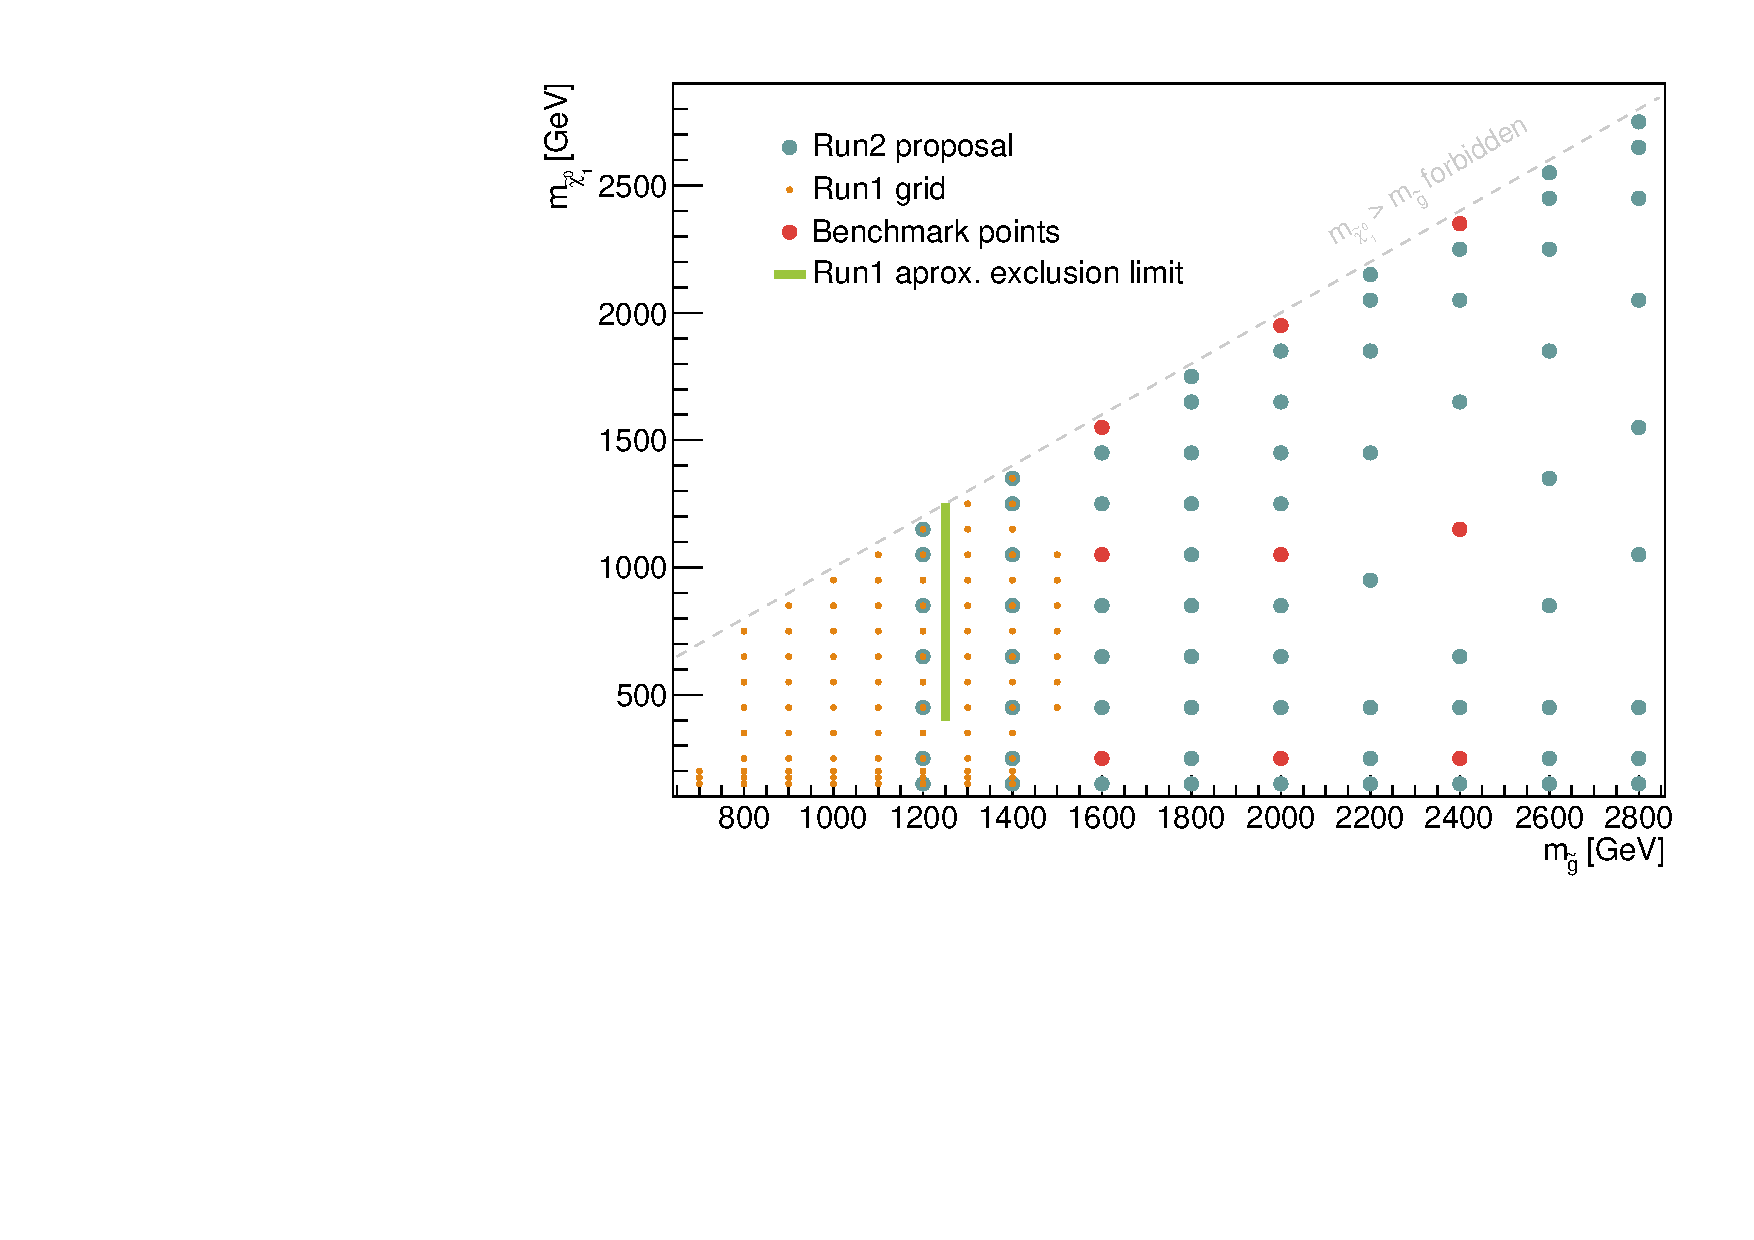
\includegraphics[width=0.6\textwidth]{images/analysis/phb_grid.pdf}
  \caption{Arreglo de muestras de señal generados en función de la masa del \ninoone y $\tilde{g}$ (celeste). La densidad del mismo disminuye al aumentar $m_{\tilde{g}}$ debido a que la sensibilidad del análisis se estimó ser menor a los \magn{2}{TeV}. En rojo se muestran los puntos empleados para realizar pruebas preliminares de sensibilidad para el presente análisis. En naranja los puntos de señal simulados para un análisis equivalente realizado durante el Run 1, que excluye las masas marcadas por la línea verde.}
  \label{fig:grid_points}
\end{figure}

\begin{sloppypar} % porque el NNLO... me quedaba en el margen
La sección eficaz de las muestras se calcula en función de la masa del \gluino a 
NNLO$_\text{approx}$+NNLL \cite{Beenakker:1996ch, Kulesza:2008jb, Kulesza:2009kq, Beenakker:2009ha, Beenakker:2011fu}. La sección eficaz nominal, junto con su incerteza, se obtienen de la combinación 
% envelope
de las distintas secciones eficaces empleando diferentes conjuntos de PDFs, y modificando los factores de renormalización y factorización, como se describe en la Referencia \cite{Borschensky:2014cia}. En la Tabla \ref{tab:gino_xs} se muestran los valores de las secciones eficaces para las distintas masas de \gluino empleadas para las muestras.
\end{sloppypar}

\begin{table}[ht!]
  \centering
  \caption{Sección eficaz de producción de pares de \gluino en función de su masa, para los distintos puntos de señal \cite{susy_xs_web}.}
  \begin{tabular}{l r r}
  \hline
  \hline
    $m_{\gluino}$    & $\sigma$(NNLO$_\text{approx}$+NNLL)[pb] &    Incerteza (\%)  \\
    \hline
    \hline
    1200 & $0.985 \cdot 10^{-01}$ & 13.03 \\
    1400 & $0.284 \cdot 10^{-01}$ & 14.44 \\
    1600 & $0.887 \cdot 10^{-02}$ & 15.94 \\
    1800 & $0.293 \cdot 10^{-02}$ & 17.56 \\
    2000 & $0.101 \cdot 10^{-02}$ & 19.42 \\
    2200 & $0.356 \cdot 10^{-03}$ & 21.83 \\
    2400 & $0.128 \cdot 10^{-03}$ & 25.19 \\
    2600 & $0.462 \cdot 10^{-04}$ & 30.31 \\
    2800 & $0.168 \cdot 10^{-04}$ & 38.48 \\
    \hline
    \hline
  \end{tabular}
  \label{tab:gino_xs}
\end{table}




% \solved{Hay mas graficos de BR para poner, hacen falta? no lo creo...} No hace falta
% \solved{mencionar como se calculo la XS} done

\section{Fondos del Modelo Estándar}\label{sec:sm_backgrounds}


Los procesos del SM que cumplen el rol de fondo para el presente análisis son aquellos que tienen el mismo estado final que la señal, es decir, fotones, jets y energía transversa faltante. Los mismos pueden ser clasificados en distintos tipos, por ejemplo, aquellos procesos que dan lugar a eventos con un fotón y energía faltante real son denominados fondos irreducibles. En dichos fondos, la energía faltante proviene de los neutrinos, y se componen principalmente de partículas que decaen a ellos, junto con fotones y jets de la ISR. Los procesos que cumplen con estos requisitos son la producción de bosones $Z$, $W$ y pares de top quarks que decaen subsecuentemente a bosones $W$:

\begin{itemize}
  \item $Z(\rightarrow \nu\nu) + \gamma + \text{jets}$
  \item $Z(\rightarrow \nu\nu) + \gamma + \gamma + \text{jets}$
  \item $W(\rightarrow l\nu) + \gamma + \text{jets}$
  \item $W(\rightarrow l\nu) + \gamma + \gamma + \text{jets}$
  \item $t\bar{t} + \gamma + \text{jets}$
\end{itemize}

Adicionalmente, es posible tener procesos que si bien no producen fotones, uno de los objetos presentes en el mismo es erróneamente reconstruido como fotón, y genere un estado final igual al buscado pero con fotones <<falsos>>. Los objetos que pueden ser erróneamente reconstruidos como fotones son los electrones y los jets. Se considera entonces aquellos procesos que no tienen fotones reales, pero se producen electrones o jets junto a neutrinos:

\begin{itemize}
  \item $Z(\rightarrow \nu\nu) + \text{jets}$
  \item $W(\rightarrow l\nu) + \text{jets}$
  \item $t\bar{t} + \text{jets}$
\end{itemize}

Por último, puede ocurrir que si bien en el proceso no hay neutrinos, una reconstrucción errónea de la energía de los distintos objetos presentes en el evento, genere un desbalance al calcular la energía transversa faltante, y por ende tengan una cantidad no despreciable de la misma, denominada energía transversa faltante instrumental. Este tipo de eventos puede ocurrir también en simultáneo junto con fotones <<falsos>>, por lo que existen diversos procesos que cumplan tales requisitos, entre los que se encuentran:

\begin{itemize}
  \item jets (denominado Multijet o QCD)
  \item $\gamma + \text{jets}$
  \item $\gamma + \gamma + \text{jets}$
  \item $Z(\rightarrow ll) + \text{jets}$
  \item $Z(\rightarrow ll) + \gamma + \text{jets}$
  \item $Z(\rightarrow ll) + \gamma + \gamma + \text{jets}$
\end{itemize}

Como notación simplificada de los fondos del análisis, se omite en el nombre tanto el <<+>> como la producción de jets en la ISR. Cabe destacar que existen más procesos que cumplen las condiciones anteriores, pero que no son considerados para el análisis. Esto se debe a que la sección eficaz es despreciable comparada con los otros procesos considerados, o el estado final se encuentra suprimido por las selecciones básicas del análisis, por lo que su contribución es completamente despreciable. Algunos ejemplos de ellos son la producción doble de bosones ($WW$, $ZZ$, $WZ$), bosones decayendo a quarks ($W(\rightarrow qq)$, $Z(\rightarrow qq)$), producción de top ($t\gamma$, $tW$), entre otros.

Para modelar los fondos con fotones <<reales>> se utilizan simulaciones de MC, mientras que para aquellos con fotones <<falsos>> se utilizan técnicas basadas en datos. 
% \solved{mencionar que para la optimizacion sí se usaron MC para los fakes?} Na...
Para los jets falseando fotones (\textit{jfakes}) se emplea un método denominado \texttt{ABCD}, y para los electrones falseando fotones (\textit{efakes}) un método denominado \texttt{Tag\&Probe}. El modelado de todos los fondos se describe en las siguientes Secciones.

\subsection{Muestras de fondo a partir de simulaciones de Monte Carlo}

Los fondos del SM con fotones <<reales>> son modelados utilizando simulaciones de MC, los cuales consisten en: \phj, \wph, \ttbarph, \wphph, \zph, \zphph, \phph. Los tres primeros son considerados de mayor impacto en el análisis y por ende son normalizados en respectivas regiones de control. Para el resto de los fondos solo se utilizan las simulaciones con las normalizaciones descriptas en la Sección \ref{sec:mc_weights}. 
% \solved{reescrito}
% Cabe mencionar que también el fondo \znunuph es considerado de alta importancia en el análisis, pero la dificultad para diseñar una región de control dedicada llevó a la decisión de utilizarlo con las normalizaciones usuales. La parte del análisis que se basa en la producción electrodébil  sí hace uso de una región de control dedicada para este análisis, y se describe en el Capítulo \ref{cap:analysis_EWK}.
Cabe mencionar que también el fondo \znunuph tiene un impacto considerable en algunas regiones del análisis, pero la dificultad de diseñar una región de control para dicho fondo sin contaminación de señal, llevó a la decisión de utilizarlo sin una normalización dedicada. 
% \solved{sigue estando mal poner normalizaciones usuales si ya lo describi en una seccion ?} Reescrito, omitiendo la palabra usuales
La parte del análisis que se basa en la producción electrodébil sí hace uso de una región de control dedicada para este fondo, debido a que el impacto de dicho proceso es mucho más elevado, como se describe en el Capítulo \ref{cap:analysis_EWK}.

Todos los procesos, salvo \ttbarph, fueron simulados utilizando el generador {\texttt{SHERPA} v2.2} \cite{Bothmann:2019yzt}. Los elementos de la matriz se calculan para un máximo de cuatro partones
a LO, y se fusionan con la lluvia de partones de \texttt{SHERPA} \cite{Schumann:2007mg} utilizando la prescripción de \texttt{MEPS@LO} \cite{Hoeche:2012yf}. La muestra de \ttbarph se genera con \texttt{MadGgraph5\_aMC@NLO} \cite{Alwall:2014hca} a segundo orden en teoría de perturbaciones (NLO), con \texttt{Pythia8} para el modelo de la lluvia de partones \cite{Sjostrand:2014zea}. 
% \solved{algún dato más debería poner, cual?}. % nope
Para todas las muestras se utilizó en la simulación del detector el programa \texttt{Geant4}. En la Tabla \ref{tab:mc_samples} se listan todas las muestras de fondos utilizadas en el análisis, las mismas se encuentran segmentadas (\textit{slicing}) según se aclara explícitamente para cada una.

\begin{table}[h!]
  \centering
  \caption{Muestras de fondos de MC utilizadas en el análisis, donde se especifica su generador, sección eficaz, $k$-factor y eficiencia de filtro.}
  \label{tab:mc_samples}
  \resizebox{\textwidth}{!}{
  \begin{tabular}{llrrr}

     \hline
      \hline
    Proceso & Generador & Sección Eficaz [pb] & $k$-factor & Eficiencia de filtro \\

    \hline
     \hline

    \ttbarph, $\pt^{\gamma} > 140$ \gev  & \texttt{MadGgraph5\_aMC@NLO}/\texttt{Pythia8} & 0.21551  & 1.0 & 1.0  \\

    \hline

    $Z(ee)\gamma$, $\pt^\gamma>140$ \gev                 & \texttt{SHERPA} v2.2.2 & 0.0634   & 1.0 & 1.0\\
    $Z(\mu\mu)\gamma$, $\pt^\gamma>140$ \gev             & \texttt{SHERPA} v2.2.2 & 0.0632   & 1.0 & 1.0\\

    $Z(\tau\tau)\gamma$, $\pt^\gamma>140$ \gev           & \texttt{SHERPA} v2.2.2 & 0.0634   & 1.0 & 1.0\\

    $Z(\nu\nu)\gamma$, $\pt^\gamma>140$ \gev             & \texttt{SHERPA} v2.2.2 & 0.2446   & 1.0 & 1.0\\

  \hline
    $W(e \nu)\gamma$, $\pt^\gamma>140$ \gev              & \texttt{SHERPA} v2.2.2 & 0.2980   & 1.0 & 1.0\\


    $W(\mu \nu)\gamma$, $\pt^\gamma>140$ \gev            & \texttt{SHERPA} v2.2.2 & 0.2987   & 1.0 & 1.0\\


    $W(\tau \nu)\gamma$, $\pt^\gamma>140$ \gev           & \texttt{SHERPA} v2.2.2 & 0.2983   & 1.0 & 1.0\\
    \hline
    \phj, $\pt^\gamma \in [70-140]$ \gev      & \texttt{SHERPA} v2.2.2 & 4526.5   & 1.0 & 1.0 \\
    \phj, $\pt^\gamma \in [140-280]$ \gev     & \texttt{SHERPA} v2.2.2 & 376.05   & 1.0 & 1.0 \\
    \phj, $\pt^\gamma \in [280-500]$ \gev     & \texttt{SHERPA} v2.2.2 & 21.851   & 1.0 & 1.0 \\
    \phj, $\pt^\gamma \in [500-1000]$ \gev    & \texttt{SHERPA} v2.2.2 & 1.4637   & 1.0 & 1.0 \\
    \phj, $\pt^\gamma \in [1000 - ]$ \gev       & \texttt{SHERPA} v2.2.2 & 0.02987  & 1.0 & 1.0 \\
    \hline
    \phph, $m_{\gamma\gamma} \in [0-50]     $ \gev         & \texttt{SHERPA} v2.2.4 & 93.499                 & 1.0 & 1.0 \\
    \phph, $m_{\gamma\gamma} \in [50-90]    $ \gev         & \texttt{SHERPA} v2.2.4 & 139.04                 & 1.0 & 1.0 \\
    \phph, $m_{\gamma\gamma} \in [90-175]   $ \gev         & \texttt{SHERPA} v2.2.4 & 51.818                 & 1.0 & 1.0 \\
    \phph, $m_{\gamma\gamma} \in [175-2000] $ \gev         & \texttt{SHERPA} v2.2.4 & 10.999                 & 1.0 & 1.0 \\
    \phph, $m_{\gamma\gamma} \in [2000-]    $ \gev         & \texttt{SHERPA} v2.2.4 & 0.0007                 & 1.0 & 1.0 \\
      \hline
      $Z(ee)\gamma\gamma$,      $\pt^{\text{sub}-\gamma} \in [9-17]$ \gev                 &  \texttt{SHERPA} v2.2.4 & $0.8705$ & 1.0 & 1.0 \\
      $Z(ee)\gamma\gamma$,      $\pt^\gamma>17$ \gev, $m_{\gamma\gamma} \in [0-80]$ \gev  &  \texttt{SHERPA} v2.2.4 & $0.1993$ & 1.0 & 1.0 \\
      $Z(ee)\gamma\gamma$,      $\pt^\gamma>17$ \gev, $m_{\gamma\gamma}>80$ \gev          &  \texttt{SHERPA} v2.2.4 & $0.0345$ & 1.0 & 1.0 \\

      $Z(\mu\mu)\gamma\gamma$,  $\pt^{\text{sub}-\gamma} \in [9-17]$ \gev                 &  \texttt{SHERPA} v2.2.4 & $0.8689$ & 1.0 & 1.0 \\
      $Z(\mu\mu)\gamma\gamma$,  $\pt^\gamma>17$ \gev, $m_{\gamma\gamma} \in [0-80]$ \gev  &  \texttt{SHERPA} v2.2.4 & $0.1999$ & 1.0 & 1.0 \\
      $Z(\mu\mu)\gamma\gamma$,  $\pt^\gamma>17$ \gev, $m_{\gamma\gamma}>80$ \gev          &  \texttt{SHERPA} v2.2.4 & $0.0346$ & 1.0 & 1.0 \\

      $Z(\tau\tau)\gamma\gamma$,$\pt^{\text{sub}-\gamma} \in [9-17]$ \gev                 &  \texttt{SHERPA} v2.2.4 & $0.8718$ & 1.0 & 1.0 \\
      $Z(\tau\tau)\gamma\gamma$,$\pt^\gamma>17$ \gev, $m_{\gamma\gamma} \in [0-80]$ \gev  &  \texttt{SHERPA} v2.2.4 & $0.2005$ & 1.0 & 1.0 \\
      $Z(\tau\tau)\gamma\gamma$,$\pt^\gamma>17$ \gev, $m_{\gamma\gamma}>80$ \gev          &  \texttt{SHERPA} v2.2.4 & $0.0345$ & 1.0 & 1.0 \\

      $Z(\nu\nu)\gamma\gamma$,  $\pt^{\text{sub}-\gamma} \in [9-17]$ \gev                 &  \texttt{SHERPA} v2.2.4 & $0.0919$ & 1.0 & 1.0 \\
      $Z(\nu\nu)\gamma\gamma$,  $\pt^\gamma>17$ \gev, $m_{\gamma\gamma} \in [0-80]$ \gev  &  \texttt{SHERPA} v2.2.4 & $0.0237$ & 1.0 & 1.0 \\
      $Z(\nu\nu)\gamma\gamma$,  $\pt^\gamma>17$ \gev, $m_{\gamma\gamma}>80$ \gev          &  \texttt{SHERPA} v2.2.4 & $0.0184$ & 1.0 & 1.0 \\
      \hline
      $W(e\nu)\gamma\gamma$,    $\pt^{\text{sub}-\gamma} \in [9-17]$ \gev                 &  \texttt{SHERPA} v2.2.4 & $0.4396$ & 1.0 & 1.0 \\
      $W(e\nu)\gamma\gamma$,    $\pt^\gamma>17$ \gev, $m_{\gamma\gamma} \in [0-80]$ \gev  &  \texttt{SHERPA} v2.2.4 & $0.0715$ & 1.0 & 1.0 \\
      $W(e\nu)\gamma\gamma$,    $\pt^\gamma>17$ \gev, $m_{\gamma\gamma}>80$ \gev          &  \texttt{SHERPA} v2.2.4 & $0.0379$ & 1.0 & 1.0 \\

      $W(\mu\nu)\gamma\gamma$,  $\pt^{\text{sub}-\gamma} \in [9-17]$ \gev                 &  \texttt{SHERPA} v2.2.4 & $0.4384$ & 1.0 & 1.0 \\
      $W(\mu\nu)\gamma\gamma$,  $\pt^\gamma>17$ \gev, $m_{\gamma\gamma} \in [0-80]$ \gev  &  \texttt{SHERPA} v2.2.4 & $0.0711$ & 1.0 & 1.0 \\
      $W(\mu\nu)\gamma\gamma$,  $\pt^\gamma>17$ \gev, $m_{\gamma\gamma}>80$ \gev          &  \texttt{SHERPA} v2.2.4 & $0.0379$ & 1.0 & 1.0 \\

      $W(\tau\nu)\gamma\gamma$, $\pt^{\text{sub}-\gamma} \in [9-17]$ \gev                 &  \texttt{SHERPA} v2.2.4 & $0.4373$ & 1.0 & 1.0 \\
      $W(\tau\nu)\gamma\gamma$, $\pt^\gamma>17$ \gev, $m_{\gamma\gamma} \in [0-80]$ \gev  &  \texttt{SHERPA} v2.2.4 & $0.0715$ & 1.0 & 1.0 \\
      $W(\tau\nu)\gamma\gamma$, $\pt^\gamma>17$ \gev, $m_{\gamma\gamma}>80$ \gev          &  \texttt{SHERPA} v2.2.4 & $0.0379$ & 1.0 & 1.0 \\
    \hline
     \hline
  \end{tabular}
  }
\end{table}

\subsection{Fondo de jets erróneamente reconstruidos como fotones}\label{sec:jfakes}

Es posible que un jet sea erróneamente reconstruido como un fotón principalmente cuando proviene de un $\pi^0$. Los piones neutros decaen rápidamente a dos fotones, que naturalmente son reconstruidos en el ECAL. Para poder distinguir el decaimiento de un pión de la producción de un fotón individual, se utiliza la primera capa del calorímetro, que tiene mayor granularidad (Sección \ref{sec:ph_id}). En el caso de que el pión se produzca con un elevado \pt, los dos fotones pueden estar muy colimados y por ende ser prácticamente indistinguibles de un fotón individual. Si bien la identificación \texttt{Tight} se encarga de suprimir en gran parte esta reconstrucción errónea, aún así puede contener una contaminación moderada de este proceso. Este tipo de fondo proviene principalmente de procesos como Multijets, $W+\text{jets}$ o de \ttbar decayendo semi-leptónicamente. 
% \solved{reescrito}
% Esta reconstrucción errónea de jets no es esperable que sea modelada correctamente mediante simulaciones de MC, por lo que se utilizan técnicas basadas en datos para estimar su contribución.
Como es extremadamente difícil modelar con precisión la tasa de errónea de jets a fotones mediante simulaciones, se emplean técnicas basadas en datos para estimar su contribución.


El método empleado para estimar este fondo se denomina \texttt{ABCD} \cite{Alonso:2233238}. El mismo hace uso de la diferencia que existe en las variables de aislamiento de fotones <<reales>> (señal en este contexto) y la de los <<falsos>> (fondo), para poder seleccionar eventos de uno u otro.
% \solved{Esto cuando se utilizaría? Me parece que mirar las formas quedó de un método viejo no? Ahora solo miramos número de eventos. O es para la correlación?} % lo cambie a variables y listo
En el contexto de este método, se definen fotones aislados como aquellos que pasan el WP \texttt{FixedCutTight},
 % \solved{esta bien esto?} Si...
 $-20\,\gev<\ETiso<0\,\gev$ y $0<\pTiso<0.05$, y los no-aislados aquellos con $8\,\gev<\ETiso<80\,\gev$ o $0.15<\pTiso<1$.
% \solved{capaz deba definir estas variables aca, o en la parte de fotones} Done, en fotones
A su vez se utiliza una selección de identificación adicional que discrimina los fotones <<reales>> \texttt{Tight} de los fotones <<falsos>>. Este criterio de identificación se denomina \texttt{Non-Tight} (denominado también \textit{pseudo-photons}, \texttt{Tight-4} o \texttt{LoosePrime}) y consiste en los fotones que pasan la selección \texttt{Loose} pero que no pasan alguno de los criterios de selección \texttt{Tight} que emplea las variables $w_{s3}$, $F_{\text{side}}$, $\Delta E$ o $E_{\text{ratio}}$. Esta selección es un subconjunto de los eventos seleccionados por el trigger de fotones \texttt{Loose}, pero completamente ortogonal a la identificación \texttt{Tight}. 

El método \texttt{ABCD}, utilizado en este análisis en particular, preselecciona eventos con al menos un fotón con $\pt>1450\,\gev$, al menos dos jets y ningún leptón, cuyos requisitos son idénticos a los que se usan en el análisis descriptos en la Sección \ref{sec:selection}. A partir de ello se definen cuatro regiones \cite{ATL-COM-PHYS-2016-1626}:

\begin{itemize}
  \item Región A: fotones \texttt{Tight} y aislados
  \item Región B: fotones \texttt{Tight} y no aislados
  \item Región C: fotones \texttt{Non-Tight} y aislados
  \item Región D: fotones \texttt{Non-Tight} y no aislados
\end{itemize}

La Figura \ref{fig:abcd_regions} muestra la distribución de datos en las variables de aislamiento para las regiones A, B, C y D. En la misma se ve explícita la brecha (\textit{gap}) que existe entre las variables de aislamiento para reducir así la contaminación entre las regiones.
 % \solved{es por esto?}. SI

\begin{figure}
  \centering
  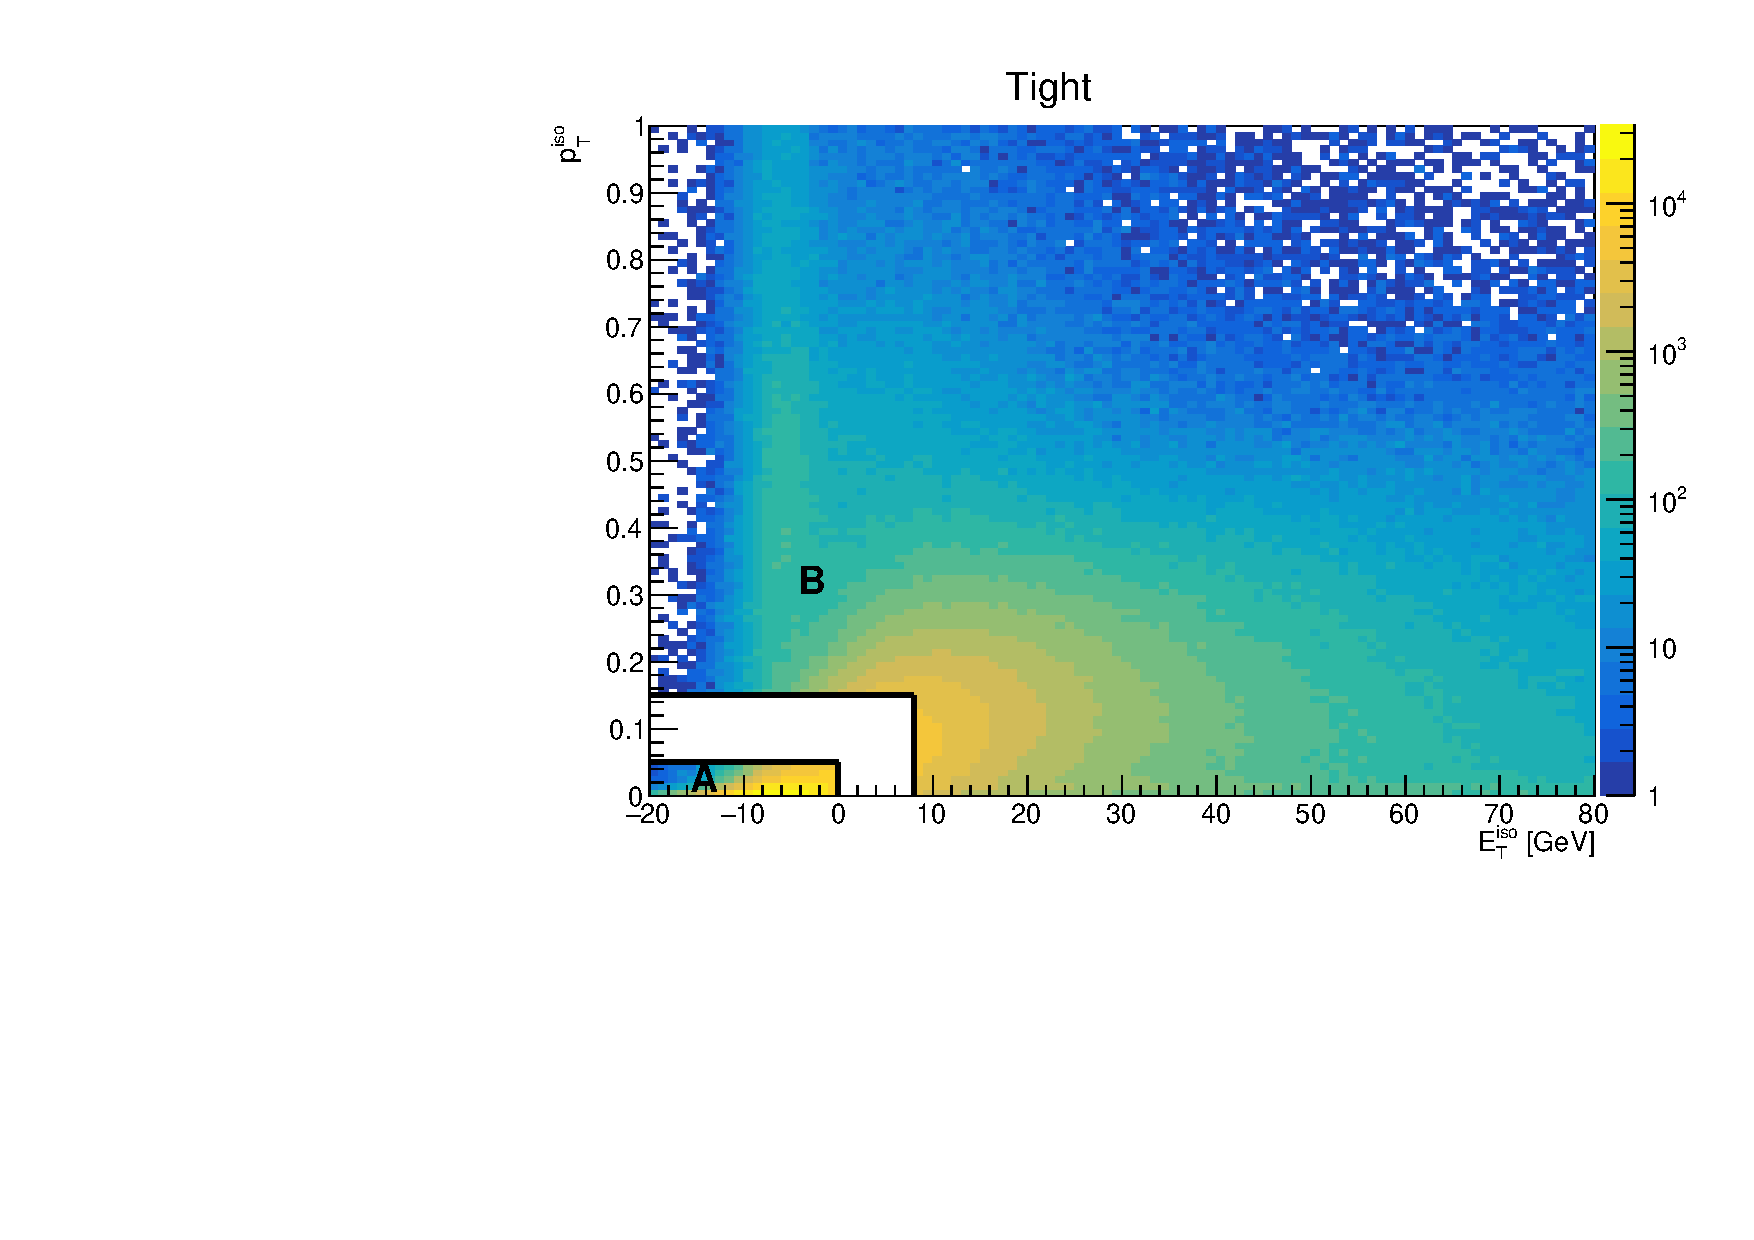
\includegraphics[width=0.45\textwidth]{images/analysis/tight_ABCD_data.pdf}
  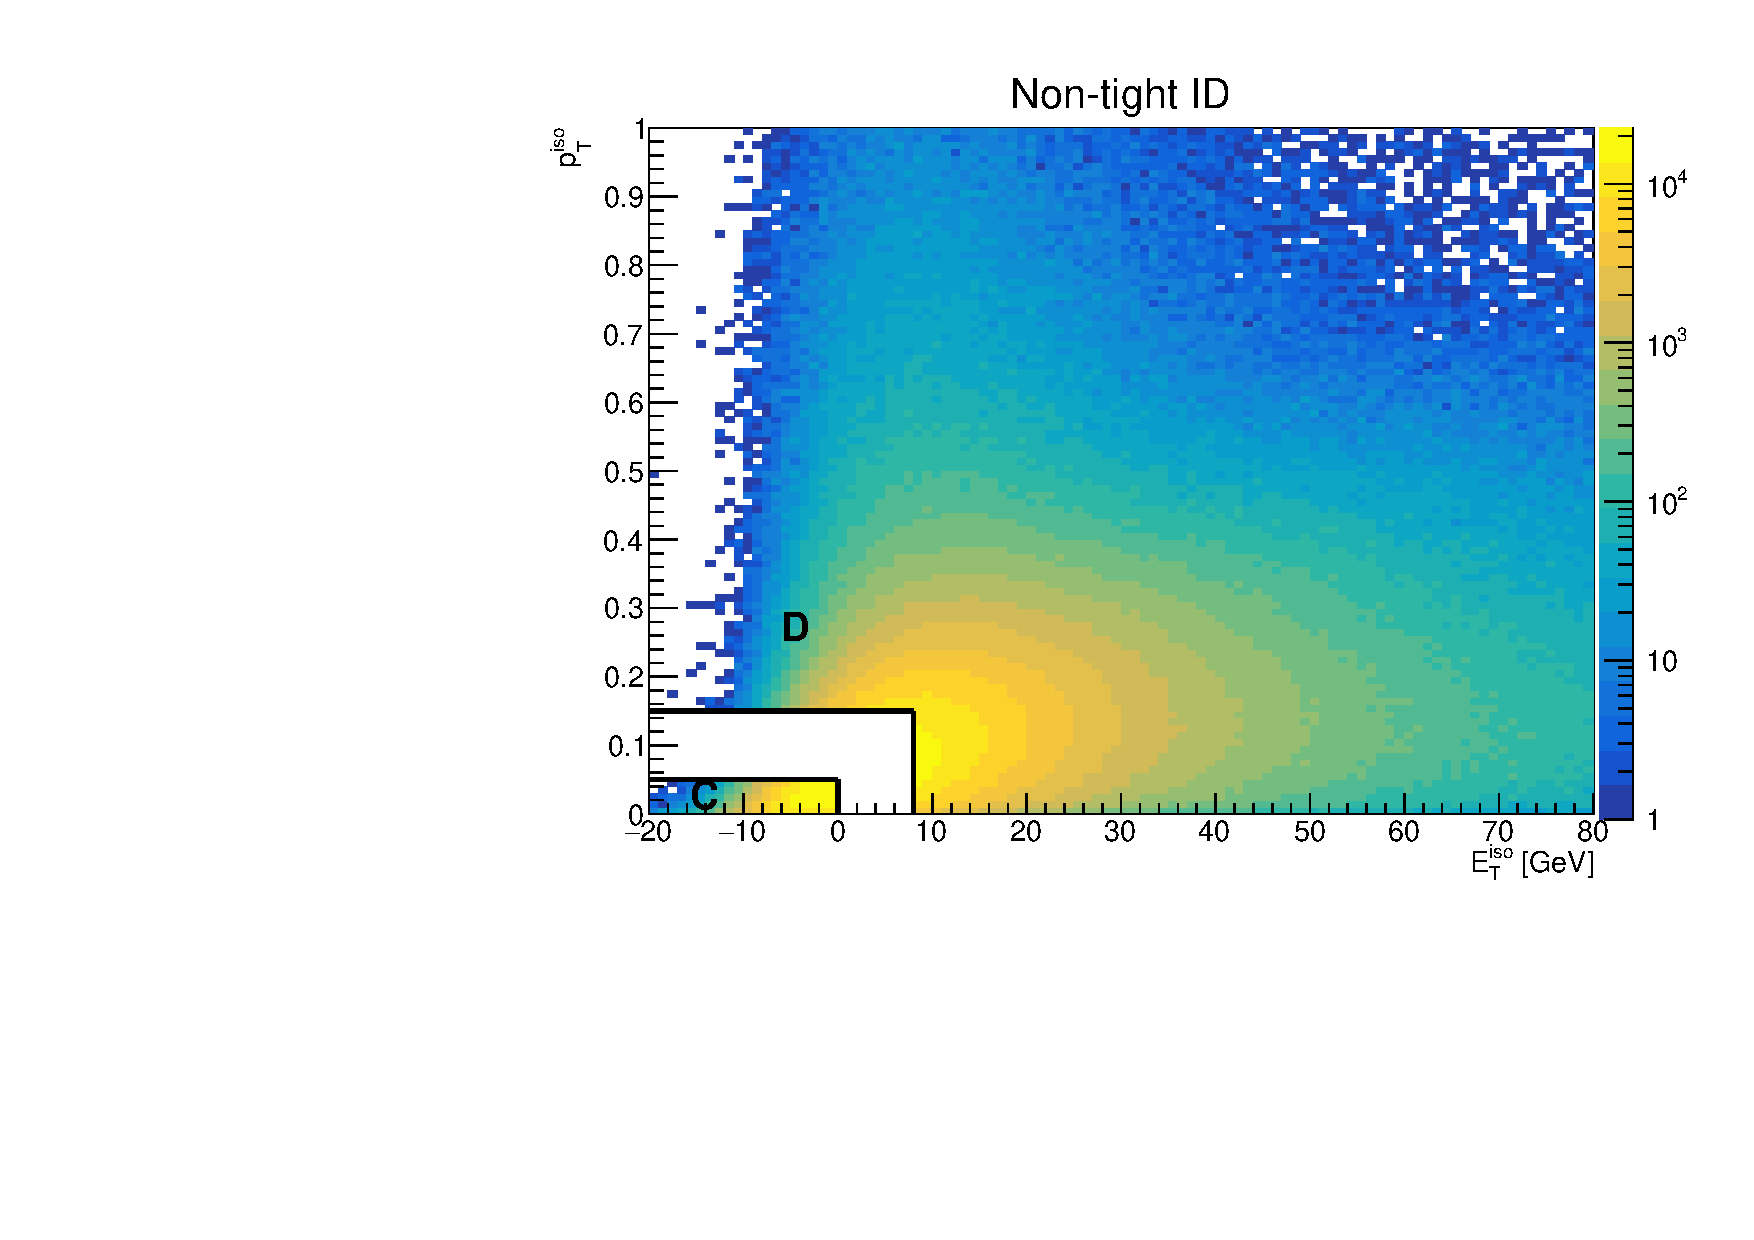
\includegraphics[width=0.45\textwidth]{images/analysis/nontight_ABCD_data.pdf}
  \caption{Distribución de datos en las variables de aislamiento para las regiones A, B, C y D.}
  \label{fig:abcd_regions}
\end{figure}


El método se basa en asumir que no hay correlación entre las variables de aislamiento y la selección de identificación \cite{tesis_tony}, y que tampoco hay contaminación de eventos de señal en las regiones B, C y D ($N_{B,C,D}=N_{B,C,D}^b$), lo que permite esperar la siguiente relación para los eventos de fondo esperados en la región A: $N_A^b / N_B = N_C/N_D$. 
% \solved{reescrito}
% Donde cada término representa el número de fondo en cada región. 
Reescribiendo la expresión anterior se puede estimar el número de fondo en la región A como:

\begin{equation}
  N_A^b = \text{FF}_{\text{iso}}\times N_B = \text{FF}_{\text{ID}}\times N_C
  \label{eq:jfakes_ff}
\end{equation}

\noindent
donde:
\begin{equation}
  \begin{split}
    \text{FF}_{\text{iso}} &= \frac{N_C}{N_D} \\
    \text{FF}_{\text{ID}} &= \frac{N_B}{N_D} \\
  \end{split}
\end{equation}

\noindent
son los denominados \textit{Fake Factors} (FF). 
Si bien ambos factores deben dar resultados equivalentes, se encuentra que al usar $\text{FF}_{\text{iso}}$ las incertezas sistemáticas se ven reducidas y por ende se decide usarlo en el análisis.

Distintas correcciones se realizan sobre este método. El primero es considerar la posibilidad de una contribución de fotones reales de señal en las regiones B, C y D. La misma se estima utilizando simulaciones de MC con fotones <<reales>> a nivel generador, y luego se resta a los datos observados, para asegurar de este modo solo el conteo de eventos de fondo en cada región. Adicionalmente, se considera una posible correlación entre variables calorimétricas y de identificación, que se puede agregar como un factor multiplicativo a la Ecuación \ref{eq:jfakes_ff}. Ese factor se define como:

\begin{equation}
  R = \frac{N_a^b N_D^b}{N_B^b N_C^b} \neq 1
\end{equation}

Debido al blinding del análisis, no es posible conocer el número de eventos observados en la región A, por lo que se calcula el factor $R$ en regiones contenidas dentro de la zona de eventos de fondo, asumiendo que tienen la misma correlación entre ellas:

\begin{equation}
  R' = \frac{N_a' N_D'}{N_B' N_C'} \neq 1
\end{equation}

\noindent
donde:
\begin{itemize}
  \item Región A: fotones \texttt{Tight}, $9\,\gev<\ETiso<15\,\gev$ y $0.2<\pTiso<0.3$
  \item Región B: fotones \texttt{Tight}, $15\,\gev<\ETiso<80\,\gev$ y $0.3<\pTiso<1$
  \item Región C: fotones \texttt{Non-Tight}, $9\,\gev<\ETiso<15\,\gev$ y $0.2<\pTiso<0.3$
  \item Región D: fotones \texttt{Non-Tight}, $15\,\gev<\ETiso<80\,\gev$ y $0.3<\pTiso<1$
\end{itemize}

\noindent
cuyas definiciones se basan en tener regiones exclusivamente con fondo, pero con una estadística suficiente.

Con estas correcciones la estimación del fondo final queda de la forma:

\begin{equation}
    N_{\jfake} = N_A^b = \left[R' \frac{N_C - N_C^s}{N_D - N_D^s} \left( 1 - \frac{N_B^s}{N_B} \right)  \right] \times N_B = \text{FF}_{\text{iso}}(\absEta, \pt, \met) \times N_B \\
\end{equation}

Los FFs se estiman en función del \pt y \absEta del fotón, y \met del evento. Distintas fuentes de incertezas sistemáticas son consideradas. 
% \solved{Motivar elecciones} anotado como pregunta de jurado
Una de ellas es cambiar la definición de la identificación \texttt{Non-Tight}, utilizando ahora \texttt{Tight-3}\footnote{Selección \texttt{Loose} que no pasa alguno de los criterios de selección \texttt{Tight} que emplea las variables $w_{s3}$, $F_{\text{side}}$ o $\Delta E$} y \texttt{Tight-5}\footnote{Selección \texttt{Loose} que no pasa alguno de los criterios de selección \texttt{Tight} que emplea las variables $w_{s3}$, $F_{\text{side}}$, $\Delta E$, $E_{\text{ratio}}$ o $w_{\text{stot}}$}. A su vez se consideran los efectos de la correlación residual, calculando los FFs con $R'=1$, e incluyendo las variaciones como sistemáticos.

En la Tabla \ref{tab:jfake_ff} se puede observar los valores de los FFs obtenidos en función del \pt y $|\eta|$ del fotón, y \met del evento. Los valores obtenidos para $R'$ dan cercanos a la unidad con desviaciones cercanas al 10\%.

El fondo para cada región (R) del análisis se estima definiendo una correspondiente región de control de jets (CSJ), que cumple el rol de la región $N_B$, y se define de igual forma que R pero reemplazando los cortes sobre fotones por jets. Se estima la contribución del fondo entonces como:

% \begin{equation}
%   N^{\text{R}}_{j\rightarrow\gamma} = \text{FF}_{\text{iso}} \cdot N^{\text{R}}_{\mathrm{CSJ}} 
%   \label{eq:jfake_cs}
% \end{equation}

\begin{equation}
  N^{\text{R}}_{j\rightarrow\gamma} = \sum_{i,j,k} \text{FF}_{\text{iso}}(|\eta_i|, p_{\text{T}\,j}, E_{\text{T}\,k}^{\text{miss}}) \cdot N^{\text{R}}_{\mathrm{CSJ}}(|\eta_i|, p_{\text{T}\,j}, E_{\text{T}\,k}^{\text{miss}})
  \label{eq:jfake_cs}
\end{equation}

\noindent
donde la suma se realiza sobre los distintos intervalos de \absEta, \pt y \met.
En el caso de no observar eventos en alguna CSJ, se hace una estimación conservadora con un evento.


\begin{table}[!ht]
  \centering
  \caption{Valores obtenidos para los factores de reconstrucción errónea de jets en fotones en función del \pt y $|\eta|$ del fotón, y \met del evento. Las incertezas son tanto estadísticas como sistemáticas.}
  \resizebox{.6\textwidth}{!}{
  \begin{tabular}{c|l|ccc}
    \hline
    \hline
      \multirow{2}{*}{$|\eta|$} & \multirow{2}{*}{{\pt} [{\gev}]}  & \multicolumn{3}{c}{\met [GeV]} \\
        & & $[50-100]$         & $[100-200]$        & $>200$              \\
    \hline
    \hline
    \multirow{6}{*}{Barrel}       & $[145-200]$   & 0.055 $\pm$ 0.008 & 0.042 $\pm$ 0.005 &  0.07 $\pm$ 0.02 \\
    & $[200-250]$ & 0.044 $\pm$ 0.005 & 0.027 $\pm$ 0.003 &  0.06 $\pm$ 0.02 \\
    & $[250-300]$ & 0.041 $\pm$ 0.003 & 0.022 $\pm$ 0.005 &  0.06 $\pm$ 0.01 \\
    & $[300-350]$ & 0.037 $\pm$ 0.004 & 0.019 $\pm$ 0.003 &  0.05 $\pm$ 0.01  \\
    & $[350-400]$ & 0.036 $\pm$ 0.003 & 0.019 $\pm$ 0.004 &  0.06 $\pm$ 0.01 \\
    & $>400$      & 0.038 $\pm$ 0.005 & 0.013 $\pm$ 0.002 &  0.05 $\pm$ 0.01  \\

    \hline
    \multirow{6}{*}{End-cap}      & $[145-200]$                      & 0.05 $\pm$ 0.02 & 0.05 $\pm$ 0.01 & 0.2 $\pm$ 0.1 \\
   & $[200-250]$ & 0.05 $\pm$ 0.01 & 0.04 $\pm$ 0.01 & 0.2 $\pm$ 0.1  \\
   & $[250-300]$ & 0.050  $\pm$ 0.008 & 0.04 $\pm$ 0.01 & 0.14 $\pm$ 0.04  \\
   & $[300-350]$ & 0.052 $\pm$ 0.009 & 0.030  $\pm$ 0.006 & 0.08  $\pm$ 0.05 \\
   & $[350-400]$ & 0.058 $\pm$ 0.007 & 0.043 $\pm$ 0.008 & 0.2 $\pm$ 0.1 \\
   & $>400$      & 0.07  $\pm$ 0.01 & 0.047 $\pm$ 0.008 & 0.14 $\pm$ 0.05 \\
    \hline
    \hline

    %     \multirow{6}{*}{Barrel}       & $[145-200]$   & 0.055 $\pm$ 0.0077 & 0.042 $\pm$ 0.0047 &  0.066 $\pm$ 0.0241 \\
    %   & $[200-250]$                      & 0.044 $\pm$ 0.0051 & 0.027 $\pm$ 0.0033 &  0.059 $\pm$ 0.0163 \\
    %   & $[250-300]$                      & 0.041 $\pm$ 0.0034 & 0.022 $\pm$ 0.0047 &  0.057 $\pm$ 0.0095 \\
    %   & $[300-350]$                      & 0.037 $\pm$ 0.0043 & 0.019 $\pm$ 0.0026 &  0.046 $\pm$ 0.014  \\
    %   & $[350-400]$                      & 0.036 $\pm$ 0.0033 & 0.019 $\pm$ 0.0035 &  0.057 $\pm$ 0.0117 \\
    %   & $>400$                           & 0.038 $\pm$ 0.0053 & 0.013 $\pm$ 0.0022 &  0.047 $\pm$ 0.011  \\

    %     \hline
    %     \multirow{6}{*}{End-cap}      & $[145-200]$                      & 0.048 $\pm$ 0.0152 & 0.053 $\pm$ 0.0139 & 0.213 $\pm$ 0.0963 \\
    %        & $[200-250]$                      & 0.045 $\pm$ 0.0114 & 0.041 $\pm$ 0.0102 & 0.226 $\pm$ 0.125  \\
    %    & $[250-300]$                      & 0.05  $\pm$ 0.0079 & 0.039 $\pm$ 0.0097 & 0.143 $\pm$ 0.043  \\
    %    & $[300-350]$                      & 0.052 $\pm$ 0.0085 & 0.03  $\pm$ 0.0058 & 0.08  $\pm$ 0.0515 \\
    %    & $[350-400]$                      & 0.058 $\pm$ 0.0071 & 0.043 $\pm$ 0.0079 & 0.179 $\pm$ 0.1064 \\
    %    & $>400$                           & 0.07  $\pm$ 0.0095 & 0.047 $\pm$ 0.0077 & 0.141 $\pm$ 0.0528 \\

  \end{tabular}
  }
  \label{tab:jfake_ff}
\end{table}



\subsection{Fondo de electrones erróneamente reconstruidos como fotones}\label{sec:efakes}

Los fotones y los electrones pueden dejar lluvias electromagnéticas muy
similares en el ECAL, cuya reconstrucción se describe en la Sección \ref{sec:ph_el}.
Si bien los algoritmos de reconstrucción de electrones y fotones están diseñados para poder discriminar uno de otros, una pequeña fracción residual de electrones puede ser reconstruida erróneamente como fotones. Si bien la reconstrucción de los clusters es altamente efectiva, la fracción de electrones mal reconstruidos se debe prácticamente a ineficiencias en la reconstrucción de trazas. Por ejemplo, la traza de un electrón puede ser mal reconstruida como un vértice de conversión, y por ende el mismo es reconstruido como un fotón convertido. O inclusive una errónea asociación de la traza con el cluster puede hacer que el electrón sea reconstruido como fotón no convertido.
Puede ocurrir a su vez, que el cluster no satisfaga los criterios de ambigüedad, y el objeto sea almacenado por duplicado como electrón y fotón. Esto en general es fácil de suprimir aplicando requisitos de solapamiento, aunque dichos requisitos pueden favorecer al electrón, y tener nuevamente en la selección del análisis electrones mal reconstruidos. Este tipo de efectos se ve principalmente en procesos como $W(l\nu)+\text{jets}$, $Z(ee)+\text{jets}$ o \ttbar. Al igual que con los jets, como es prácticamente imposible estimar esta reconstrucción errónea con simulaciones de MC, se utiliza una técnica basada en datos para estimar dicha fracción de reconstrucción errónea. Para ello se utiliza una muestra de eventos con producción de bosones $Z$, como el mismo no puede decaer a $e+\gamma$, los eventos con este par de partículas y que parecieran provenir del decaimiento de un $Z$, son un buen indicio de que ese fotón en realidad es un electrón mal reconstruido. En ese caso se puede estimar una fracción de reconstrucción errónea (Fake Factor, FF) como:

\begin{equation}
  F_{e\to \gamma} \equiv \frac{P(e^{\text{real}}\to \gamma^{\text{reco}})}{P(e^{\text{real}}\to e^{\text{reco}})}  = \frac{\epsilon(e^{\text{real}}\to \gamma^{\text{reco}})}{\epsilon(e^{\text{real}}\to e^{\text{reco}})} \frac{\epsilon^{\text{ID}}_{\gamma}}{\epsilon^{\text{ID}}_{e}} = \frac{N_{e^{\text{real}}\to \gamma^{\text{reco}}}}{N_{e^{\text{real}}\to e^{\text{reco}}}} \frac{\epsilon^{\text{ID}}_{\gamma}}{\epsilon^{\text{ID}}_{e}}
  \label{eq:efake_ff}
\end{equation} 

\noindent
donde $P(e\to e(\gamma))$ es la probabilidad de reconstruir e identificar un electrón <<real>> como un electrón (fotón), $\epsilon(e^{\text{real}}\to e(\gamma)^{\text{reco}})$ es la eficiencia de reconstruir un electrón <<real>> como un electrón (fotón)\footnote{Definida como $\frac{N_{e^{\text{real}}\to e(\gamma)^{\text{reco}}}}{N_{e^{\text{real}}\to e^{\text{reco}}}+N_{e^{\text{real}}\to \gamma^{\text{reco}}}}$}, $\epsilon^{\text{ID}}_{e} (\epsilon^{\text{ID}}_{\gamma})$ es la eficiencia de identificar un electrón (fotón), y $N_{\text{real}\ e\to \text{reco}\ e(\gamma)}$ el número electrones reconstruidos como electrones (fotones). Como no es posible saber a partir de los datos cuándo un electrón es <<real>>, este factor debe ser estimado a partir de los objetos ya reconstruidos y sus eficiencias, magnitudes que sí son mensurables en datos. Para una dada muestra con eventos de bosones $Z$, la probabilidad de reconstruir a sus productos de decaimiento como pares $ee$ o $e\gamma$ esta dada por:
% \solved{tengo que pensar mejor estas fórmulas, pero va por aca la cosa} O sea están bien, se omitio un paso nomas que se basa en el footnote...

\begin{equation}
\begin{split}
\frac{N_{ee}}{N_Z} & = (\epsilon^{ID}_{e})^{2} (1-\epsilon(e^{\text{true}}\to \gamma^{\text{reco}}))^{2} \\
\frac{N_{e\gamma}}{N_Z} & = \epsilon^{ID}_{e}\epsilon^{ID}_{\gamma} (1-\epsilon(e^{\text{true}}\to \gamma^{\text{reco}}))\epsilon(e^{\text{true}}\to \gamma^{\text{reco}}) \\
\end{split}
\end{equation}


Usando la Ecuación \ref{eq:efake_ff} se puede escribir al FF en función de los objetos reconstruidos a partir de los decaimientos de bosones $Z$:

\begin{equation}
  F_{e\to \gamma}(|\eta|) = \frac{N_{e\gamma}(|\eta^{\gamma}|)}{N_{ee}(|\eta^{e}|)}
\end{equation}


El método para estimar los FFs, denominado \texttt{Tag\&Probe} \cite{tesis_gonza}, emplea una muestra a partir de todos los datos tomados durante el Run 2, seleccionando aquellos que contengan al menos dos electrones, o al menos un electrón y un fotón. En el caso de múltiples posibles pares en el evento, se utiliza la combinación cuya masa invariante esté más cerca de $m_Z=91.1876\,\gev$ \cite{ParticleDataGroup:2018ovx}. A su vez, se aplica un corte con $\met<40\,\gev$ para suprimir eventos con $W$ decayendo a electrones. Los requisitos de los objetos son idénticos a los que se usan en el análisis descriptos en la Sección \ref{sec:selection}.

Para identificar si el par proviene del decaimiento de un bosón $Z$ se reconstruye su masa invariante, de forma separada, dependiendo si el par es $ee$ o $e\gamma$. Como el FF se calcula en función de $|\eta|$, se obtienen distribuciones de la masa invariante de cada par, para distintos intervalos de $|\eta|$ como se describe en la Figura \ref{fig:efakes_matrix}. En estas selecciones, puede ocurrir que haya un conjunto de eventos que no provenga del $Z$ (fondo no resonante), por lo que se ajusta una función del tipo <<señal+fondo>> a cada distribución de masa. Para la señal se utiliza una función del tipo \textit{Double-sided crystal ball}\footnote{La misma se define como una Gaussiana, cuyas colas se modifican por funciones potenciales. Los parámetros libres son la media y desviación estándar de la Gaussiana, junto con los factores de cada potencia y las fronteras donde se juntan con la Gaussiana} \cite{Das:2016stf} y para el fondo una función Gaussiana.

\begin{figure}
  \centering
  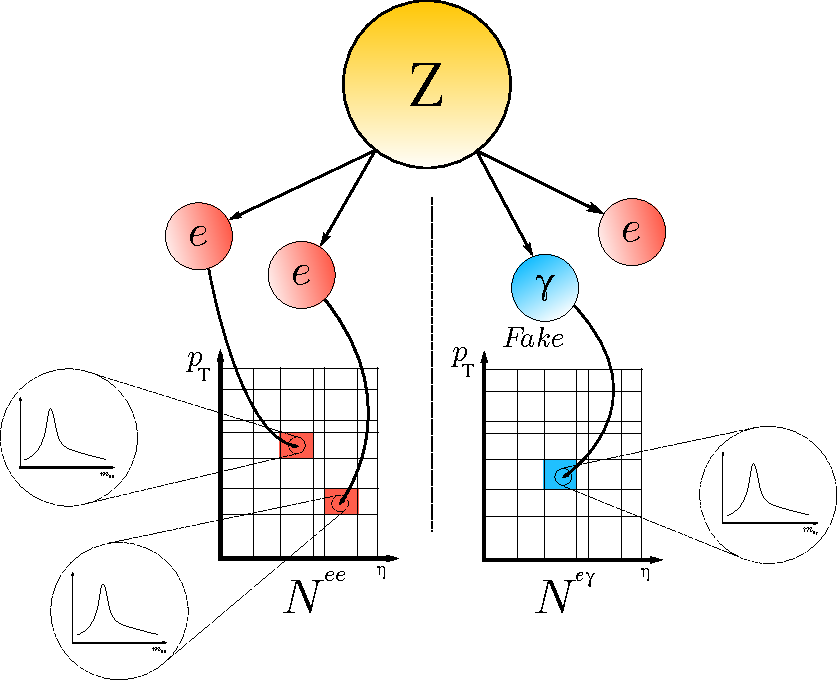
\includegraphics[width=0.6\textwidth]{images/analysis/grid_en_2.pdf}
  \caption{Esquema de reconstrucción de las distintas distribuciones de masa invariante utilizadas en el método. La clasificación en \pt de la imagen proviene de un método similar anterior, y actualmente solo se emplea una clasificación en \absEta. Tanto las distribuciones de pares con fotón leading como de los pares con fotón sub-leading son almacenadas, pero no se hace explícito en la imagen.}
  \label{fig:efakes_matrix}
\end{figure}

Una vez ajustada cada distribución, la función se integra alrededor del pico del $Z$ en una ventana definida como $[\mu - 3\sigma, \mu + 3\sigma]$, para obtener el número de eventos que se emplea en los factores de la Ecuación \ref{eq:efake_ff}, para cada intervalo de $|\eta|$. En la Figura \ref{fig:efakes_fit} se puede observar el resultado del ajuste para la distribución de masa invariante de pares $ee$ y $e\gamma$, con $|\eta| \in [0-0.6]$. 
% \solved{reescrito}
% Cabe mencionar que anteriormente el método empleada una clasificación adicional en \pt, y que eso introducía un sesgo en las distribuciones que era contemplado agregando una función Gaussiana adicional, centrada en valores. Como actualmente se aplica un corte en $\pt>145\,\gev$ el efecto del mismo es completamente despreciable para los eventos cerca del pico del $Z$.
Cabe mencionar que al aplicar un corte en $\pt>145\,\gev$ se introduce un sesgo en la distribución de la masa invariante de los pares, el cual se considera despreciable dada su lejanía con el pico del $Z$. Dicho efecto se observa en la región de masas de \magn{300}{GeV}, para el cual se incluye una función Gaussiana adicional al fondo, centrada en esa zona.


\begin{figure}[ht!]
  \centering
  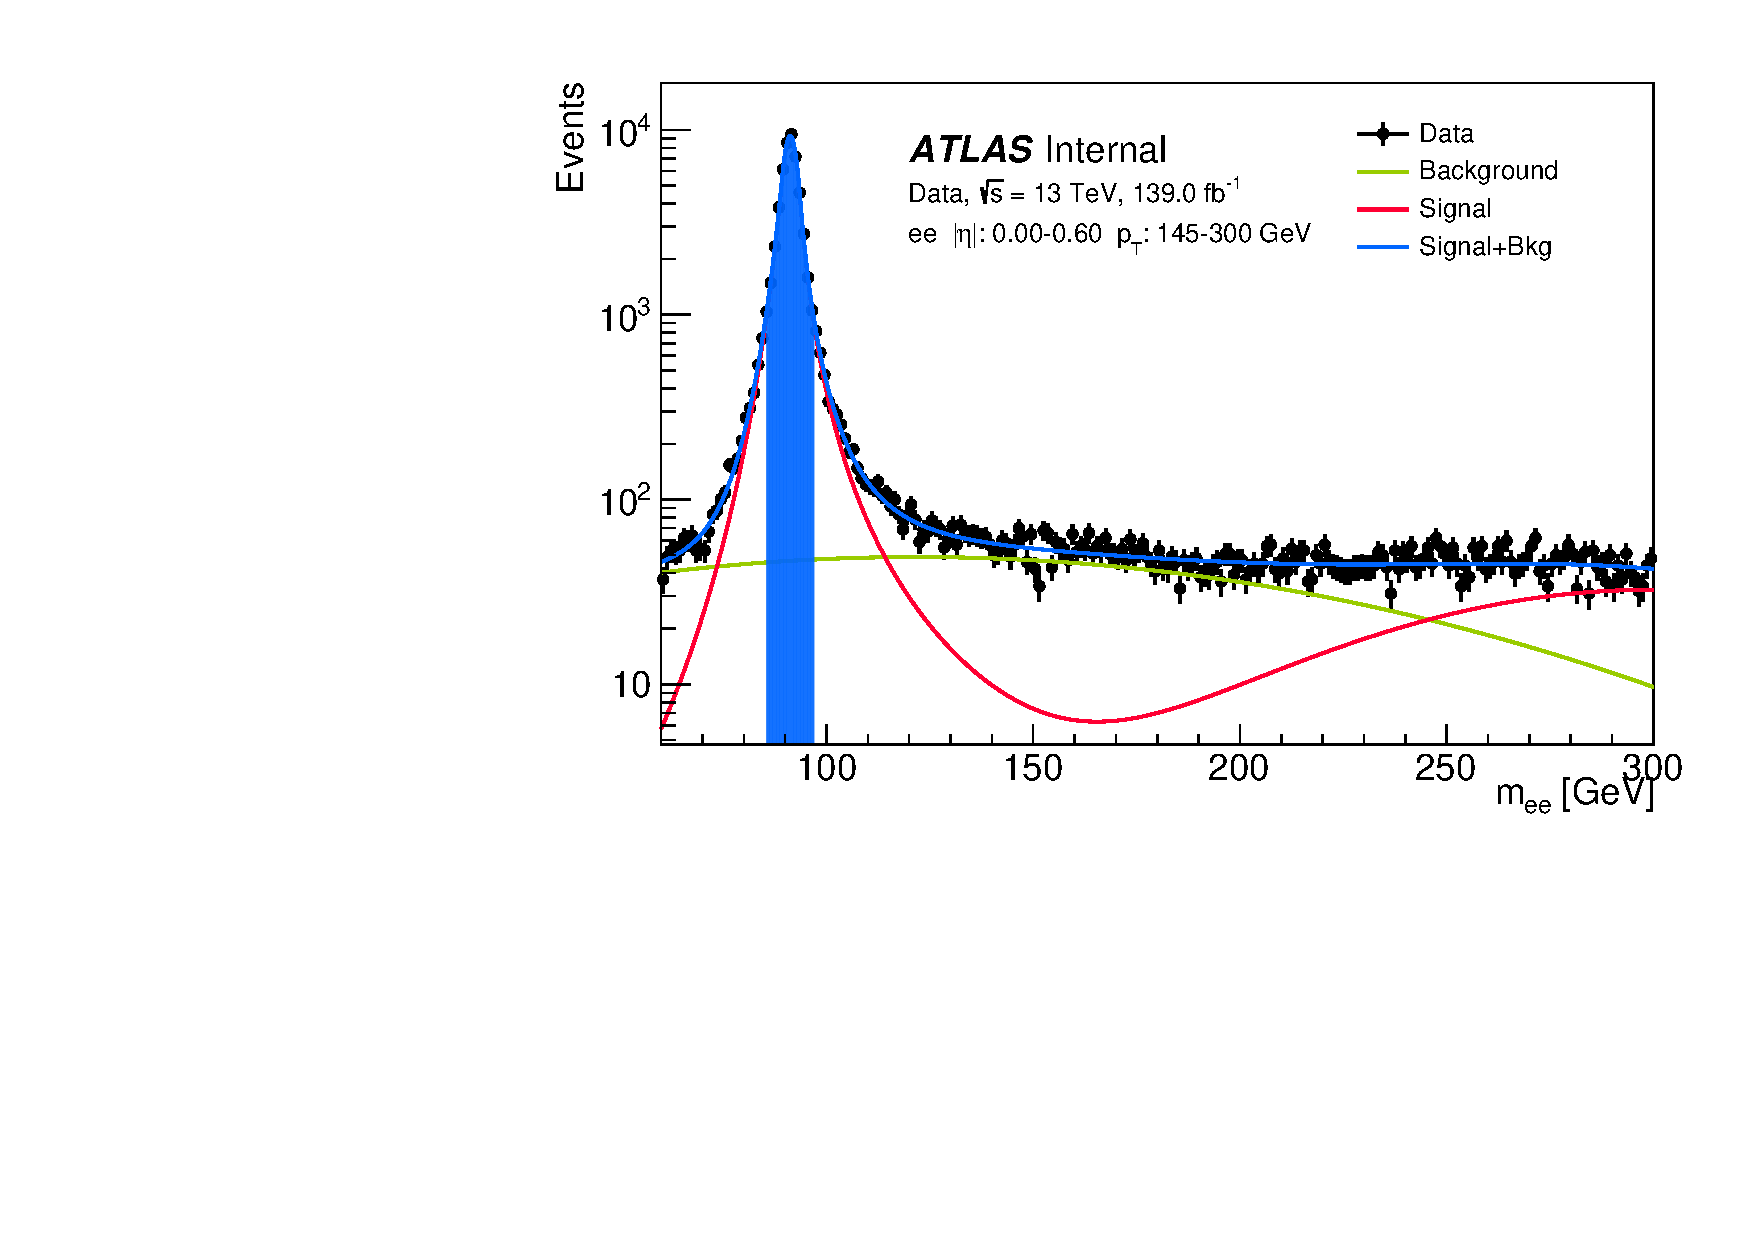
\includegraphics[width=0.45\textwidth]{images/analysis/egFF_fit_ee_eta_0_06.pdf}
  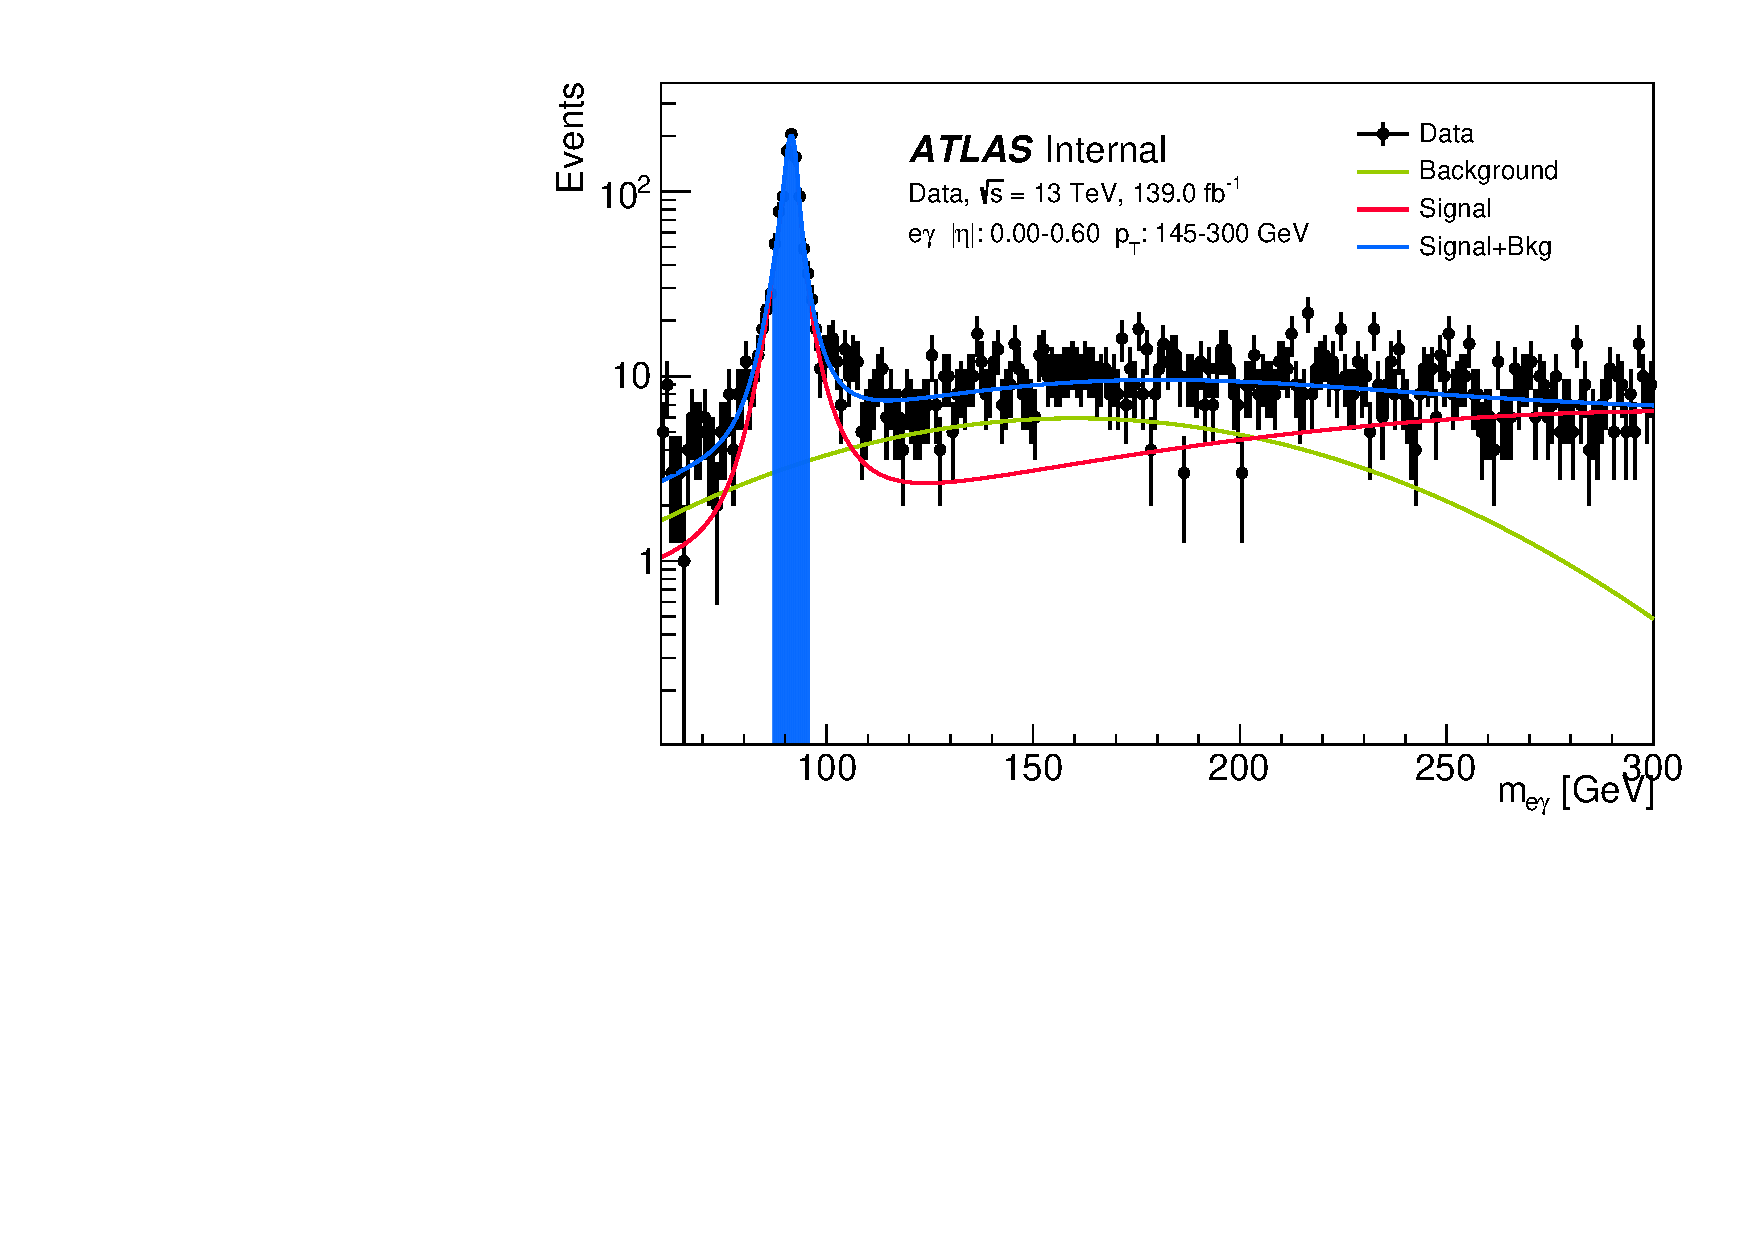
\includegraphics[width=0.45\textwidth]{images/analysis/egFF_fit_eg_eta_0_06.pdf}
  \caption{Distribución de la masa invariante para los pares $ee$ (izquierda) and $e\gamma$ (derecha) con $|\eta| \in [0-0.6]$, junto con las funciones ajustadas de señal (rojo) y fondo (verde). La región celeste representa la ventana de integración empleada para calcular los FFs. A alto \pt, una Gaussiana adicional es incluida para tener en cuenta el sesgo al aplicar un corte en dicha variable, que resulta despreciable su contribución en el número de eventos cerca del pico del $Z$.}
  \label{fig:efakes_fit}
\end{figure}


La incerteza sistemática se estima variando las ventanas de integración a $[\mu - 2\sigma, \mu + 2\sigma]$ y $[\mu - 4\sigma, \mu + 4\sigma]$. Adicionalmente se calculan los FFs sin la sustracción del fondo, incluyendo esta variación como un sistemático que contempla el sesgo en la elección de la función de ajuste. Finalmente, como la energía del fotón <<falso>> es reconstruida con algoritmos para fotones, cuando en realidad deberían haber sido empleados los de electrones, se considera esto como una incerteza sistemática. Para ellos se calculan nuevamente los FFs ahora modificando el valor de energía de los fotones en un factor 1.5\%. Dicho valor se obtiene de las diferencias que existen entre el $\mu$ de las distribuciones con pares $ee$ y pares $e\gamma$ \cite{EXOT-2016-32}. Los valores obtenidos para los FFs junto con sus incertezas se pueden observar en la Tabla \ref{tab:efakes_ff}. Se puede ver como los mismos aumentan con $|\eta|$, relacionados con la cantidad de material que atraviesan y con la mayor fracción de reconstrucción de fotones convertidos con una sola traza.


\begin{table}
\centering
\caption{Factores de reconstrucción errónea de electrones como fotones en función de $|\eta|$ para todos los datos del Run 2. Se muestran explícitas las incertezas estadísticas y sistemáticas provenientes de variar la ventana de integración, no emplear la sustracción de fondo y el sesgo en la energía de los fotones.}
\resizebox{\textwidth}{!}{
\begin{tabular}{ l | c | c c c c | c }
\hline
\hline
\multirow{2}{*}{$|\eta|$} & \multirow{2}{*}{Fake factor} & incerteza & \multicolumn{3}{c |}{incerteza sistemática} & incerteza \\
\cline{4-6}
 & & estadística. & V. integración & Sin sustracción & Sesgo energía & Total\\
\hline
\hline
0.00-0.60 & 0.019 & 0.0001 & 0.0001 & 0.0006 & 0.001 & 0.001 \\
0.60-1.37 & 0.024 & 0.0001 & 0.0003 & 0.001 & 0.0001 & 0.001 \\
1.52-1.82 & 0.050 & 0.0001 & 0.0000 & 0.0009 & 0.003 & 0.003 \\
1.82-2.37 & 0.086 & 0.0001 & 0.0007 & 0.002 & 0.005 & 0.005 \\
\hline
\hline

% 0.00-0.60 & 0.0194 & 0.0000 & 0.0001 & 0.0006 & 0.0012 & 0.0013 \\
% 0.60-1.37 & 0.0244 & 0.0000 & 0.0003 & 0.0014 & 0.0001 & 0.0014 \\
% 1.52-1.82 & 0.0497 & 0.0001 & 0.0000 & 0.0009 & 0.0028 & 0.0029 \\
% 1.82-2.37 & 0.0863 & 0.0001 & 0.0007 & 0.0016 & 0.0051 & 0.0054 \\

\end{tabular}
}
\label{tab:efakes_ff}
\end{table}


Finalmente, el fondo para cada región (R) del análisis se estima definiendo una correspondiente región de control de electrones (CSE), definida de igual forma que R pero reemplazando los cortes sobre fotones por electrones. Se estima la contribución del fondo entonces como:

% \solved{no me convence poner (\absEta) en los siguientes terminos} creo que podria poner una sumatoria de bines, es algo menor. ponele que asi esta bien...

% \begin{equation}
%   N^{\text{R}}_{e\rightarrow\gamma} = \text{FF}_{e\to\gamma} \cdot N^{\text{R}}_{\mathrm{CSE}} 
%   \label{eq:efake_cs}
% \end{equation}

\begin{equation}
  N^{\text{R}}_{e\rightarrow\gamma} = \sum_{i} \text{FF}_{e\to\gamma}(|\eta_i|) \cdot N^{\text{R}}_{\mathrm{CSE}} (|\eta_i|)
  \label{eq:efake_cs}
\end{equation}

\noindent
donde la suma se realiza sobre los distintos intervalos de \absEta.
En el caso de no observar eventos en alguna CSE, se hace una estimación conservadora con un evento.
% \solved{no sabia esto!!!}. Era importante cuando no teniamos eventos en algunas regiones en 2016, ahora no pasa eso

% \solved{esto tambien se hace para jfakes, por que nunca lo hacemos explicito?} Agregar


\section{Selección de eventos y objetos para el análisis}\label{sec:selection}

El presente análisis hace uso de la totalidad de datos con una energía de centro de masa de \magn{13}{TeV}, tomados con el detector ATLAS durante el Run 2 y que son <<aptos para física>>, acumulando una luminosidad total integrada de $139\,\ifb$. Los datos son seleccionados a partir del trigger \texttt{HLT\_g140\_loose}, que selecciona eventos con al menos un fotón con identificación \texttt{Loose} y con $\ET>140\,\gev$. Este trigger es completamente eficiente \cite{TRIG-2018-05}, superando el 99\% de eficiencia para $\ET>145\,\gev$, estable frente a pile-up y sin dependencia en $\eta$.

Los datos y simulaciones de MC empleados para el análisis son preseleccionados con la derivación \texttt{SUSY1} descripta en la Sección \ref{sec:lhc_samples}, orientada a análisis con moderada actividad hadrónica y con la presencia de un fotón energético entre otras cosas.

Los objetos de interés para esta Tesis son los fotones, jets y leptones (electrones y muones) a los que se les aplica diferentes requisitos offline. Inicialmente se les requiere una selección base (\textit{baseline}),
que se emplea para aplicar un requisito de solapamiento (\textit{overlap removal}) entre los distintos objetos del evento.
A su vez se les aplica una selección denominada \textit{signal}, siendo estas últimas las que definen los objetos empleados en las definiciones de las regiones del análisis. Adicionalmente, a los fondos de MC se les aplica una selección a nivel generador para evitar un solapamiento o doble conteo entre muestras. Por ejemplo, a las muestras de \zph, \wph, \ttbarph y \phj, se les solicita que tengan uno y solo un fotón a nivel generador, y en cambio a las \zphph y \wphph dos fotones. 

% \solved{mencionar a VgammaORTool} Done

% \solved{como son cortos, capaz los siguientes items podrían ser subsubsection} Yep

\subsubsection{Fotones}

Los fotones baseline deben pasar la selección de identificación \texttt{Tight}, tener $\ET>25\,\gev$, $|\eta|<2.37$ excluyendo la región del crack. Para los fotones signal se requiere adicionalmente tener $\ET>50\,\gev$, aunque para la selección de las regiones se pide adicionalmente que el fotón leading tenga $\ET>145\,\gev$ para garantizar la eficiencia del trigger. Adicionalmente se les aplica un requisito de aislamiento tanto calorimétrico como de traza, mediante el WP \texttt{FixedCutTight}.


\subsubsection{Electrones}

A los electrones baseline se los selecciona con $\pt>10\,\gev$, $|\eta|<2.47$ excluyendo la región crack, y ser originados en el vértice primario. El requerimiento de identificación \texttt{Loose}
% \solved{en realidad es LooseAndBLayerLLH} 
es aplicado. Los electrones signal son seleccionados además, con un $\pt>25\,\gev$, aplicando la identificación \texttt{Tight}
% \solved{en realidad es TightLLH} 
y el requisito de aislamiento \texttt{FCLoose}, o \texttt{FCHighPtCaloOnly} si tienen $\pt>200\,\gev$.


\subsubsection{Muon}

Los muones baseline son seleccionados con la identificación \texttt{Medium}, tener $\pt>10\,\gev$, $|\eta|<2.7$ y ser originados del vértice primario. A los muones signal se les requiere adicionalmente tener $\pt>25\,\gev$ y el WP de aislamiento \texttt{FixedCutLoose}.
% \solved{en realidad es Loose\_VarRad pero no encuentro su definición y es muy probable que sea igual a FixedCutLoose} 


\subsubsection{Jets}

Se emplean Jets \texttt{EMTopo} reconstruidos con el algoritmo \textit{anti-$k_t$} con $R=0.4$, y la selección baseline se define como aquellos con $\pt>30\,\gev$ y $|\eta|<2.8$. Este último requisito no es empleado en el cálculo de \met. Selecciones basadas en las trazas son aplicadas para rechazar jets con $\pt<120\,\gev$ y $|\eta|<2.4$ que se originen de las interacciones de pile-up \cite{ATL-PHYS-PUB-2014-001}. Jets signal son seleccionados con $\pt>30\,\gev$ y $|\eta|<2.5$. La identificación de $b$-jets es empleada en la definición de algunas regiones de control. Para ello se utiliza el algoritmo \texttt{MV2c10}, con una eficiencia de selección de los mismos del 77\%.

\subsubsection{Overlap removal}

Como se mencionó en capítulos anteriores, los algoritmos de reconstrucción pueden fallar en los criterios de ambigüedad entre objetos, decidiendo almacenar simultáneamente a ambos. Una forma de lidiar con esto es eliminando al objeto que comparta alguna región espacial del detector con otro, en lo que se denomina overlap removal \cite{Adams:1743654}. Esta eliminación se hace en diferentes pasos, y en cada uno hay un objeto eliminado en presencia de otro. Los objetos eliminados en un dado paso no influyen en los sucesivos.
El overlap removal está diseñado específicamente para el tipo de análisis \cite{ATL-COM-PHYS-2016-1518}, y los diferentes pasos aplicados en el presente análisis se resumen a continuación: 

\begin{itemize}
  \item se remueven aquellos muones CT que compartan traza con algún electrón
  \item se remueven aquellos electrones que compartan traza con algún muon
  \item se remueven aquellos fotones que tengan $\Delta R<0.4$ con algún electrón
  \item se remueven aquellos fotones que tengan $\Delta R<0.4$ con algún muón
  \item se remueven aquellos jets que tengan $\Delta R<0.2$ con algún electrón
  \item se remueven aquellos electrones que tengan $\Delta R<0.4$ con algún jet
  \item se remueven aquellos jets con número de trazas menor a 3 y que tengan $\Delta R<0.2$ con algún muón
  \item se remueven aquellos muones que tengan $\Delta R<0.4$ con algún jet
  \item se remueven aquellos jets que tengan $\Delta R<0.4$ con algún fotón
\end{itemize}


\subsubsection{Energía transversa faltante}

El cálculo de \met se realiza de acuerdo a lo descripto en la Sección \ref{sec:met}. Los depósitos de energía en el calorímetro son asociados a los objetos de alto \pt en el siguiente orden: electrones, fotones, jets y muones. Las trazas que no fueron asociadas con ninguno de los objetos anteriores, son incluidas en el término soft. Durante el análisis, una vez hecha la selección final de los objetos, se hace una selección de eventos con $\met>50\,\gev$.
% \solved{chequear}. Yep, pero solo para MC, ni aclarar igual


\section{Definición de las regiones del análisis}

Una vez obtenidas las muestras de señal y una primera estimación de los fondos del SM, el objetivo del análisis es poder diseñar regiones de señal que permitan hacer una discriminación entre ambos. Para ello se obtiene del espacio de parámetros, la combinación de requisitos o cortes que maximiza la significancia esperada, descripta en la Sección \ref{sec:exp_sig}.
La optimización se realiza en primera instancia conociendo a priori la cinemática del estado final del fondo y señal, y luego mediante un proceso iterativo para encontrar los valores de cortes más óptimos. Al maximizar significancia, se intenta además, no tener regiones muy dependientes del modelo. Con el objetivo de evitar problemas extremos de baja estadística, que causen problemas en el manejo de los sistemáticos, se buscan regiones que no tengan un número de eventos de fondo nulo, poniéndose un mínimo requerido de tres eventos. A su vez se realiza una estimación conservadora de las incertezas sistemáticas del 30\% del fondo total estimado.

Una vez definidas las SRs, se procede a la definición de las regiones de control y validación, que determinan un paso clave en el análisis para poder lograr un correcto modelado de los fondos. Las CRs se diseñan para normalizar los fondos principales del análisis, mediante un ajuste de solo fondo a los datos. Las VRs, en cambio, son diseñadas cubriendo el espacio de parámetros entre las SRs y las CRs, con el objetivo de verificar que el modelado de los fondos, y su extrapolación a las VRs, es correcto. Como ambas hacen uso de los datos, es indispensable que las mismas sean ortogonales a las SR para evitar un posible sesgo en los resultados finales, garantizando así las condiciones para el blinding.
A continuación, se detallan los pasos que se siguieron en la optimización, hasta el diseño final de las SRs y sus respectivas CRs y VRs.

\subsection{Selección de eventos de señal}\label{sec:sig_selection}

El estado final del modelo bajo estudio consiste en al menos un fotón, presencia de jets y elevada \met, como describe el diagrama de la Figura \ref{fig:phb_feyn}. 
Se seleccionan los eventos con al menos un fotón mediante 
el trigger de fotones simple con menor umbral y sin prescale, el cual es el \texttt{HLT\_g140\_loose}, por lo que a todos los fotones leading de las regiones se les solicita tener $\pt>145\,\gev$, donde el trigger es completamente eficiente. Una selección inclusiva en el número de fotones contempla el caso en el que ambos \ninoone decaen mediante fotones. El decaimiento a \gravino produce grandes cantidades de \met, que se espera que sea al menos mayor a \magn{200}{GeV}, un valor bastante más alto que los procesos usuales del SM. 
Los jets del estado final pueden provenir de los decaimientos de los \chinoonepm o \ninotwo, de la ISR o del decaimiento del Higgs, mientras que \met y los fotones provienen del \ninoone.
A grandes rasgos, la cinemática del evento depende de la diferencia de masa entre el \gluino y el \ninoone. 
Cuando la diferencia supera los {$\smallsim$}\magn{1000}{GeV}, el \gluino decae en etapas sucesivas hasta llegar al \ninoone, generando jets adicionales. A su vez, los productos del decaimiento del \ninoone son poco energéticos. En cambio, cuando la diferencia de masa es menor a {$\smallsim$}\magn{300}{GeV} (escenario comprimido), el \gluino decae en mayor proporción de forma directa al \ninoone. En ese caso se generan menos jets en el evento, y tanto el \pt del fotón como \met van a ser relativamente más energéticos.
% \solved{descripto}
% Si la diferencia es pequeña , por lo que la cadena será corta y el número de jets bajo. En cambio si la diferencia es grande, el gluino tiene otros gauginos intermedios para decaer hasta el \ninoone, por lo que lo hará más en múltiples etapas dejando un número de jets mayor. A su vez esta diferencia afecta al \pt del fotón y a \met. En el escenario comprimido, la masa del neutralino es relativamente alta y por ende el producto de sus decaimientos pueden ser más energéticos. A diferencia del caso con masas de neutralino bajas, donde se esperan fotones de menor \pt y menor \met. 
Estas diferencias entre los distintos puntos de señal motivó al diseño de tres regiones de señal, optimizadas para distintos puntos de señal. La SRH, optimizada para el escenario comprimido, caracterizada por fotones y \met energéticos, y bajo número de jets. En contraposición, está la SRL optimizada para masas de \ninoone baja, y caracterizada por un mayor número de jets, y con fotones y \met no tan energéticos. Finalmente la SRM fue optimizada para un región intermedia y con características conjuntas de las anteriores SRs. La Figura \ref{fig:sr_design} muestra el espacio de puntos para los cuales fue diseñada cada SR. Finalmente, si bien se pueden generar leptones en el estado final, se aplica un veto a los mismos para evitar el solapamiento con otro análisis que realiza una búsqueda similar con fotones y leptones en el estado final \cite{diph_8TeV}.

\begin{figure}[ht!]
  \centering
  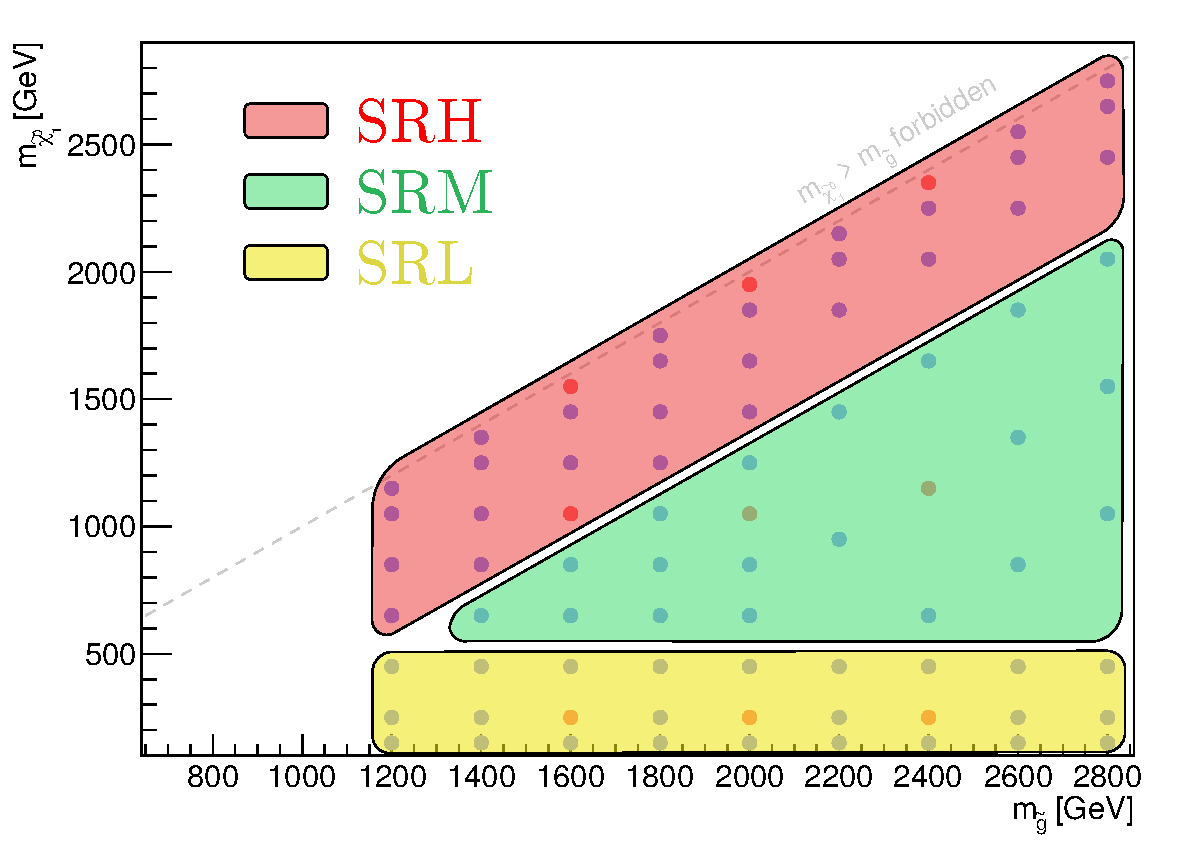
\includegraphics[width=0.5\textwidth]{images/analysis/sr_design.pdf}
  \caption{Regiones en el espacio de masas del \gluino y \ninoone para los cuales se optimiza cada región de señal. La SRH está dedicada al escenario comprimido, la SRL para la región de baja masa del \ninoone, y la SRM como una región intermedia entre las dos anteriores.}
  \label{fig:sr_design}
\end{figure}

% \solved{La aplicación y explicación de estos cortes no tendría que ir antes de la optimización ?} se referia a que la optimizacion se hace sobre las varaibles que no son fijas, en realidad ninguna esta fija, solo el numero de fotones. ademas ni se menciona la palabra optimizacion

Definidas las selecciones caracterizadas por el estado final del modelo, se procede a agregar variables que hagan efectiva la discriminación de fondo y señal. Para reducir fondos donde \met es principalmente instrumental, se aplica una separación angular entre la misma y los objetos presentes en el evento. En la señal, \met proviene principalmente de los \gravino, que se espera que no tenga ninguna correlación angular con los fotones y jets. En cambio, en procesos donde \met proviene de la reconstrucción errónea de alguno de los objetos, es esperable que la misma esté alineada con ese mismo objeto. Por ese motivo se aplica un corte inferior en las siguientes variables:

\begin{equation}
  \begin{split}
  \dphigammet & = \phi^{\text{leading}\: \gamma} - \phi^{\text{miss}} \\
  \dphijetmet & = \text{min}(\phi^{\text{leading}\: \text{jet}} - \phi^{\text{miss}}, \phi^{\text{sub-leading}\: \text{jet}} - \phi^{\text{miss}}) \\
  \end{split}
\end{equation}

\noindent
donde las diferencias se definen de tal forma de que resulten siempre entre $0$ y $\pi$.

Para una mejor discriminación entre señal y fondo se emplea la variable $\HT$, definida como:

\begin{equation}
  \HT = \ptph + \sum_{i \in \text{jets}} p_{\text{T}}^{(i)}
\end{equation}

Para una señal de SUSY con un fotón energético y elevada actividad hadrónica, se pueden esperar valores de \HT superiores a $1500\,\gev$.

Finalmente, para realizar una reducción de fondo adicional, se emplea la variable:

\begin{equation}
  R_{\text{T}}^{N} = \frac{\sum_{i=1}^{N} p_{\text{T}}^{(\text{jet}_i)}}{\sum_{i \in \text{jets}} p_{\text{T}}^{(i)}}
\end{equation}

\noindent
donde $1\le N \le N_{\text{jets}}$, que representa la fracción de \pt de los primeros $N$ jets con respecto a la totalidad de jets. Para el presente análisis se encuentra que la variable \rtf daba los valores más óptimos de significancia. Las señales de SUSY se espera que contengan eventos con múltiples jets energéticos, y por ende valores bajos de \rtf, a diferencia de los procesos del SM con baja actividad hadrónica y de baja energía, con valores de \rtf cercanos a la unidad. Cabe destacar que esta variable solo es posible definirla en regiones que soliciten al menos cuatro jets.
% \solved{mencionar lo que paso con el analisis phb? que se pensaba que los bjets del higgs podian llegar a servir para una nueva SR pero la imposibildiad de reconstruirlos correctamente no presentaba ninguna ventaja con estas SR, que en definitiva ya eran sensibles al analisis} Nope
La definición formal de las regiones de señales se muestra en la Tabla \ref{tab:sr_def}.

\begin{table}[ht!]
  \centering
  \caption{Definición de las regiones de señal SRL, SRM y SRH}
  \begin{tabular}{l|r|r|r}
    \hline
    \hline
      &        SRL    &       SRM     &         SRH \\
      \hline
      \hline
      $N_{\text{fotones}}$  & $\ge1$ & $\ge1$ & $\ge1$ \\
      \ptph&  $>145\,\gev$ &  $>300\,\gev$ &  $>400\,\gev$ \\
      $N_{\text{leptones}}$ & 0 & 0 & 0 \\
      \njet&       $\ge 5$ &       $\ge 5$ &       $\ge 3$ \\
      \dphijetmet &        $>0.4$ &        $>0.4$ &        $>0.4$ \\
      \dphigammet &        $>0.4$ &        $>0.4$ &        $>0.4$ \\
      \met&  $>250\,\gev$ &  $>300\,\gev$ &  $>600\,\gev$ \\
      \HT& $>2000\,\gev$ & $>1600\,\gev$ & $>1600\,\gev$ \\
      \rtf &       $<0.90$ &       $<0.90$ &             - \\
      \hline
      \hline
    \end{tabular}
  \label{tab:sr_def}
\end{table}




\subsection{Regiones de control y validación}\label{sec:cr_vr_sel}

En el presente análisis los procesos de mayor impacto son \phj, \wph y \ttbarph, para los cuales se diseñan regiones de control dedicadas a los mismos, denominadas CRQ, CRW y CRT respectivamente. Todas las CRs requieren al menos un fotón con $\pt>145\,\gev$ y luego un conjunto de cortes que no solo generen una buena estadística del fondo a modelar, sino también garanticen la ortogonalidad con las SRs. El corte en \HT en general es reducido con respecto a las SRs para aumentar así la estadística de los fondos, y por la misma razón el corte en \rtf se omite en todas ellas. 
Si bien algunos análisis definen regiones de control dedicadas a diferentes procesos para cada región de señal, en el análisis actual se emplean las mismas CRs para todas las SRs.
% \solved{resscrito}
% Cabe destacar que las tres regiones de control fueron empleadas para todas las regiones de señal, a diferencia de otros análisis donde hacen uso de CRs dedicadas además para cada SR.

La producción de pares de top, en su decaimiento leptónico, genera un estado final con dos $b$-jets, dos leptones y \met. La CRT dedicada a este proceso requiere entonces la presencia de al menos dos $b$-jets y un leptón, garantizando así la ortogonalidad con las SRs. Para evitar contaminación de señal se emplea un corte superior en \met, ya que para este proceso se espera que no sea tan alta como en la señal de SUSY. 
La CRW, dedicada a \wph, se diseña de forma similar a la CRT, pero aplicando un veto en los $b$-jets para evitar una contaminación del fondo de \ttbarph.

En los procesos como \phj, donde \met es principalmente instrumental, se espera que el vector \met esté alineado con alguno de los jets. La CRQ aplica un corte superior en \dphijetmet para incrementar la abundancia de este fondo, garantizando también la ortogonalidad con las SRs. Si bien \met es baja para este proceso, como hay suficiente estadística, se aplica un corte inferior en la misma para tener mayor semejanza con las SRs.
En la Tabla \ref{tab:cr_def} se muestra la definición completa de las tres regiones de control. 

% \solved{mostrar signal contamination?}. nope


\begin{table}[ht!]
  \centering
  \caption{Definición de las regiones de control de control CRQ, CRW y CRT, dedicadas a los fondos \phj, \wph y \ttbarph respectivamente. En color se resaltan los cortes que garantizan la ortogonalidad con las SRs.}
  \begin{tabular}{l|r|r|r}
    \hline
    \hline
    &   CRQ    & CRW &    CRT  \\
    \hline
    \hline
    $N_{\text{fotones}}$ &   $\ge1$    &     $\ge1$ &    $\ge1$            \\
    \ptph &  $>145\,\gev$      & $>145\,\gev$ & $>145\,\gev$                  \\
    $N_{\text{leptones}}$ &   0  & \cellcolor{lightgreen} {$\ge1$}     & \cellcolor{lightgreen} {$\ge1$} \\
    \njet     &   $\ge3$   &     $\ge1$ &    $\ge2$ \\
    \nbjet   &  -   &   $0$ &   $\ge 2$ \\
    \dphijetmet  & \cellcolor{lightgreen} {$<0.4$} &     $>0.4$ &    $>0.4$ \\
    \dphigammet   &    $>0.4$   &   - &        - \\
    \met &  $>100\,\gev$  & \cellcolor{lightgreen} {$[100,200]\ {\gev}$} & \cellcolor{lightgreen} {$[50,200]\ {\gev}$} \\
    \HT &  $>1600\,\gev$ &  $>400\,\gev$  &  $>400\,\gev$      \\
    \hline
    \hline
  \end{tabular}
  \label{tab:cr_def}
\end{table}



A continuación, se definen las VRs, las cuales fueron diseñadas para verificar el correcto modelado de los fondos, y su extrapolación a las SRs. Las mismas se encuentran en una región intermedia entre las CRs y las SRs, siempre siendo ortogonales a estas últimas. Se diseñaron un conjunto de VRs orientadas al modelado de los fondos de \wph y \ttbarph, otras para el de \phj, y una dedicada al fondo de electrones erróneamente reconstruidos como fotones. Nuevamente se requiere en todas ellas al menos un fotón con $\pt>145\,\gev$.

Se definieron cinco VRs orientadas al fondo de \phj. Estas regiones recuperan el corte en \dphijetmet de las SRs, pero agregan un corte superior en \met de $200\,\gev$, siendo así ortogonales a ellas. Entre dichas regiones se encuentran las VRM1L y VRM1H, orientadas a validar las regiones SRL y SRH respectivamente, emulando sus cortes en \pt del fotón y \met. A su vez la VRM1L incluye un corte similar en \rtf para validar la aplicación del mismo en las SRs. Ambas tienen un corte inferior en \met de $100\,\gev$, y se desprenden de ambas, regiones de validación equivalentes pero con un corte inferior en \met de $150\,\gev$, denominadas VRM2L y VRM2H. Finalmente se encuentra la VRQ, que es un compromiso entre las regiones anteriores, solicitando un reducido número de jets y a su vez el mínimo \pt para fotones. La definición completa de las VRs dedicadas al fondo de \phj se muestra en la Tabla \ref{tab:vrm_def}.


\begin{table}[ht!]
  \centering
  \caption{Definición de las regiones de validación VRQ, VRM1L, VRM2L, VRM1H y VRM2H, empleadas para la validación del fondo de \phj. En color se resaltan los cortes que garantizan la ortogonalidad con las SRs.}
  %% \resizebox{\textwidth}{!}{
    \begin{tabular}{l|r|r|r|r|r}
    \hline
    \hline
    &   VRQ & VRM1L & VRM2L & VRM1H & VRM2H \\
    \hline
    \hline
    $N_{\text{fotones}}$ & $\ge1$ & $\ge1$  & $\ge1$  & $\ge1$  & $\ge1$\\
    $\pt^{\text{leading}-\gamma}$ & $>145\,\gev$ & $>145\,\gev$  & $>145\,\gev$  & $>300\,\gev$ & $>300\,\gev$           \\
    $N_{\text{leptones}}$ &  0 & 0 & 0 & 0 & 0 \\
    \njet & $\ge3$  & $\ge5$  & $\ge5$ & $\ge3$ & $\ge3$ \\
    \dphijetmet & $>0.4$ & $>0.4$ & $>0.4$ & $>0.4$ & $>0.4$ \\
    \dphigammet &  $>0.4$ & $>0.4$ & $>0.4$ & $>0.4$ & $>0.4$ \\
    \met &  \cellcolor{lightgreen} $[100,200]$ &  \cellcolor{lightgreen} $[100,200]$ &  \cellcolor{lightgreen} $[150,200]$ & \cellcolor{lightgreen} $[100,200]$ & \cellcolor{lightgreen} $[150,200]$ \\
    \HT & $>1600$ & $>1600$  & $>1600$ & $>1600$  & $>1600$\\
    \rtf &  -  &  $<0.90$ &  $<0.90$ & - & - \\
    \hline
    \hline
    \end{tabular}
    % }
    \label{tab:vrm_def}
\end{table}


Para los fondos \wph y \ttbarph se definieron cuatro regiones de validación, por lo que todas requieren al menos un leptón, lo que las hace ortogonales a las SRs. La VRL1 y VRL2 estudian la región de bajo \met, validando distintos valores de \HT, mientras que las VRL3 y VRL4 lo hacen para $\met>200\,\gev$. Además VRL4 invierte el corte en \dphijetmet para validar esa variable en regiones con combinaciones distintas de la misma. La Tabla \ref{tab:vrl_def} muestras las definiciones completas de las VRs dedicadas a estos fondos.

\begin{table}[ht!]
  \centering
  \caption{Definición de las regiones de validación VRL1, VRL2, VRL3 y VRL4, empleadas para la validación de los fondos de \wph y \ttbarph. En color se resaltan los cortes que garantizan la ortogonalidad con las SRs.}
  \begin{tabular}{l|r|r|r|r}
  \hline
  \hline
   & VRL1 & VRL2 & VRL3  &  VRL4     \\
  \hline
  \hline
  $N_{\text{fotones}}$  &  $\ge1$ &   $\ge1$  &    $\ge1$   &  $\ge1$     \\
  $\pt^{\text{leading}-\gamma}$   &   $>145\,\gev$  &  $>145\,\gev$   & $>145\,\gev$  &  $>145\,\gev$  \\
  $N_{\text{leptones}}$   & \cellcolor{lightgreen}{$\ge1$}  & \cellcolor{lightgreen}{$\ge1$} & \cellcolor{lightgreen}{$\ge1$}  & \cellcolor{lightgreen}{$\ge1$}  \\
  \njet   &   $\ge2$ &  $\ge2$  & $\ge2$   &   $\ge2$     \\
  \dphijetmet & $>0.4$  &  $>0.4$  & $>0.4$   & \cellcolor{lightgreen}{$<0.4$}  \\
  \met & \cellcolor{lightgreen}{$[50,200]\,\gev$} & \cellcolor{lightgreen}{$[50,200]\,\gev$} &  $>200\,\gev$  &   $>200\,\gev$     \\
  \HT &  $>800\,\gev$ &  $>1300\,\gev$   & \cellcolor{lightgreen}{$[600,1600]\,\gev$} &  $>1100\,\gev$  \\
  \hline
  \hline
  \end{tabular}
  \label{tab:vrl_def}
\end{table}


Finalmente se encuentra la región de validación para el fondo de electrones erróneamente reconstruidos como fotones (VRE). La misma se diseña sin el veto de leptones y requiriendo al menos un $b$-jet. Como es un fondo donde el fotón es <<falso>>, se espera que su energía no esté correctamente reconstruida y esto genere \met instrumental. En ese caso \met y el fotón deberían estar alineados, por lo que se aplica un corte superior en \dphigammet, garantizando a su vez la ortogonalidad con las SRs. La definición de la misma se puede observar en la Tabla \ref{tab:vre_def}.


\begin{table}[ht!]
  \centering
  \caption{Definición de la región de validación VRE, empleada para la validación del fondo de electrones erróneamente reconstruidos como fotones. En color se resaltan los cortes que garantizan la ortogonalidad con las SRs.}

  \begin{tabular}{l|r}
    \hline
    \hline
    & VRE \\
    \hline
    \hline
    $N_{\text{fotones}}$                  &       $\ge1$                     \\
    \ptph         &    $145\gev$                     \\
    $N_{\text{leptones}}$                  &           -                      \\
    \njet                     &       $\ge1$                     \\
    \nbjet                   &       $\ge1$                     \\
    \dphijetmet          &       $>0.4$                     \\
    \dphigammet                &\cellcolor{lightgreen} {$<0.4$}               \\
    \met                                &   $>200\,\gev$                   \\
    \HT                                &\cellcolor{lightgreen} {$[100, 1600]\,\gev$}  \\
    \hline
    \hline
  \end{tabular}
  \label{tab:vre_def}
\end{table}


\section{Incertezas sistemáticas}

Un factor clave en el análisis es la estimación de las incertezas sistemáticas involucradas, las cuales afectan tanto la estimación de los fondos como de la señal en las distintas regiones del análisis. Las mismas son incluidas como parámetros nuisance en los distintos ajustes realizados, llegando a ser del orden de 60 incertezas. Existen dos tipos de incertezas sistemáticas, las experimentales y las teóricas, y se describen a continuación.


\subsection{Incertezas sistemáticas experimentales}

Las incertezas experimentales están asociadas a la estimación de los fondos, ya sea por incertezas provenientes de la simulación del detector, en la reconstrucción y calibración de objetos, correcciones por pile-up, medida de la luminosidad, como también en los métodos de estimación de fondos basados en datos.


\subsubsection{Incerteza en la luminosidad}

La luminosidad del LHC durante el Run 2 se mide utilizando el detector de Cherenkov LUCID2 \cite{Avoni:2018iuv}, y se calibra a partir tomas de datos especiales de baja luminosidad del LHC, utilizando el método van der Meer \cite{vanderMeer:296752,Grafstrom:2153734}. La misma es empleada en general para la medida de secciones eficaces, aunque en este análisis cumple un rol fundamental en la normalización de las simulaciones de MC a las condiciones del Run 2 del LHC. La incerteza en la luminosidad integrada combinada del Run 2 es de $1.7$\% \cite{ATLAS-CONF-2019-021}.


\subsubsection{Incertezas asociadas a fotones, electrones y muones}

Las incertezas en la identificación y aislamiento de fotones son estimadas a partir de las diferencias que hay en las \textit{shower shapes}
% \solved{no se si esta definido} Si
entre datos y MC, utilizando eventos de bosón $Z$ decayendo radiativamente \cite{PERF-2013-04}. La escala de energía es determinada utilizando eventos de $Z\to ee$ y $J/\Psi \to ee$, y sus correcciones fueron aplicadas como variaciones de una desviación estándar del valor nominal. La misma metodología se emplea para las variaciones en la resolución.
De manera similar se obtienen los sistemáticos asociados a electrones \cite{ATLAS-CONF-2014-032} y muones \cite{PERF-2015-10}, los cuales se determinan a partir de eventos $Z\to l^+l^-$, $J/\Psi\to l^+l^-$ y $W\to l^\pm \nu$. 
Las incertezas consideradas para electrones son la variación de la escala de su momento, y variaciones en la incerteza del factor de escala de reconstrucción, identificación y aislamiento.
Para muones son consideran las variaciones en la escala y resolución de su momento 
% (\textit{smearing} de la traza en el ID/MS)
, en la dependencia escala del momento con la carga, en la incerteza del factor de escala de reconstrucción y aislamiento, en los factores de escala de asociación entre traza y vértices, y el rechazo de muones con baja resolución de momento.


\subsubsection{Incertezas asociadas a jets}

Las incertezas asociadas a jets se estiman siguiendo la metodología descripta en las Referencias \cite{PERF-2011-03} y \cite{ATLAS-CONF-2015-037}, las cuales provienen de múltiples fuentes y aportan una gran cantidad de parámetros nuisance. 

% Entre ellas están la incerteza asociadas a la resolución y escala de energía, las eficiencias de identificación de sabor del jet y la incerteza en el JVT. 

Entre ellas están la incerteza asociadas a la resolución de energía, obtenida a partir de la variación del \textit{smearing} de jets de MC a datos para la corrección de la resolución, usando eventos con dos jets y datos sin sesgo de trigger mediante conos aleatorios.
% \solved{esto es un monton jaja} % ya fue
La variación de la escala de energía, proveniente de la intercalibración en $\eta$ de eventos con dos jets, balance \zj, balance \phj, balance Multijet, y de incertezas asociadas a la propagación de partículas individuales, el haz de prueba, pile-up, identificación de sabor y fuga hadrónica.
% falto MC non-closure, no se traducirla
Finalmente se consideran incertezas asociadas a la eficiencia de la identificación de sabor del jet, y de la contaminación residual de jets luego de la supresión de pile-up (JVT) y la elección del generador de MC.

% \solved{agregar mas detalles, capaz en leptones tambien}. Done

\subsubsection{Incertezas asociadas a \met}

Cuando se modifica la escala o resolución de energía de algún objeto, esta variación se propaga en conjunto al término correspondiente al cálculo de \met. Adicionalmente los sistemáticos asociados al término soft de \met se obtienen mediante la comparación de la escala y resolución entre datos y MC, con distintos generadores y simulaciones de detector.

\subsubsection{Incertezas asociadas al pile-up}

El factor de corrección de pile-up se obtiene para hacer coincidir el número promedio de interacciones por cruces de haces de las simulaciones de MC con la de datos. El mismo es de $1/1.03$, y la incerteza sistemática se obtiene variando el mismo a $1/0.99$ y $1/1.07$. 
% \solved{Esto nunca lo expliqué y no lo sé bien, seguro que se aplica estas variaciones?} consultar con fran. a leer bien

\subsubsection{Incertezas en los métodos de estimación de fondos basados en datos}

Los métodos para la estimación de fondos de jets y electrones reconstruidos erróneamente como fotones, descriptos en las Secciones \ref{sec:jfakes} y \ref{sec:efakes}, tienen también incertezas asociadas. Una es la incerteza estadística propia de la muestra de control, empleada para la estimación final de estos fondos (Ecuaciones \ref{eq:jfake_cs} y \ref{eq:efake_cs}), y que se incluye como parámetro nuisance. A su vez, la incerteza proveniente del cálculo FFs, descripta en esas mismas Secciones, es considerada como incerteza sistemática.


\subsection{Incertezas sistemáticas teóricas}

Las incertezas teóricas afectan a todas las simulaciones de MC, y provienen principalmente tanto del generador empleado, como de los distintos parámetros de la teoría utilizados en los cálculos de las propias simulaciones. 

Para cada muestra de fondo, en cada región del análisis, se calcula una incerteza teórica total que incluye los efectos que más adelante se describen. Contrario a lo que se espera, las incertezas sistemáticas se ven afectadas por la estadística de la muestra, principalmente cuando la región tiene bajo número de eventos. Es por esto, que para el cálculo de las incertezas teóricas, se emplean regiones equivalentes a la del análisis pero relajando varios de sus cortes, eliminando así la dependencia con la estadística. Se emplea una región para sistemáticos común a todas las SRs del análisis, y una para cada grupo de VRs, las cuales se muestran en la Tabla \ref{tab:syst_reg}. Para las CRs se usan exactamente las mismas ya que por definición abundan los eventos de un dado fondo.

\begin{table}[ht!]
  \caption{Regiones empleadas para el cálculo de los sistemáticos teóricos. Las mismas fueron obtenidas a partir de las regiones del análisis, pero relajando algunos de sus cortes. Para las CRs se emplearon las mismas regiones del análisis por lo que no son mostradas.}
  \centering
   % \resizebox{.9\textwidth}{!}{
    \begin{tabular}{l|r|r|r|r}
    \hline
    \hline
      & SR\_syst & VRM\_syst   & VRL\_syst & VRE\_syst   \\
      \hline
      \hline
      $N_{\text{fotones}}$              & $\ge1$   & $\ge1$      & $\ge1$    &  $\ge1$      \\
      \ptph [\gev] & $>145$   & $>300$      & $>145$    &  $>145$      \\
      $N_{\text{leptones}}$              &      0   &     0       & $>0$      &     -        \\
      \njet                 & $\ge3$   & $\ge3$      & $\ge2$    &  $\ge1$      \\
      \nbjet               &     -    &      -      &    -      &  $\ge1$      \\
      \dphijetmet      &     -    &      -      &    -      &  $>0.4$      \\
      \dphigammet          & $>0.4$   & $>0.4$      &    -      &     -        \\
      \met [\gev]                         & $>200$   & $>100$      & $>100$    &  $>200$      \\
      \HT  [\gev]                         & $>1600$  & $>1000$     & $>800$    &  [100-1600]  \\
      \hline
      \hline
    \end{tabular}
    % }
\label{tab:syst_reg}
\end{table}

Todas las muestras de fondo se generan con un conjunto de pesos internos, que al aplicarlo a cada evento, representan el efecto que generaría la variación de distintos parámetros de la teoría. Las variaciones consideradas para cada muestra son las de la escala de renormalización ($\mu_R$) y factorización ($\mu_F$), la variación de los elementos de matriz (ME) de la PDF nominal, variación de la familia de PDFs empleada en la generación de los eventos, y las incertezas asociadas a la determinación y truncamiento de la constante de acoplamiento fuerte ($\alpha_S$). Para la muestra de \ttbarph, se emplean solo las dos primeras variaciones, las cuales son las predominantes. Tampoco se tienen en cuenta variaciones en la escala de \textit{matching} (CKKW),
 % \solved{mirar esto}  a estudiar, algo puse igual en la tesis
 ni en la escala de resumación (QSF), ya que las mismas son despreciables y requieren la generación de muestras adicionales. 

\begin{sloppypar} % porque el muR muF me quedaba en el margen
El cálculo de la incerteza teórica total se realiza siguiendo las recomendaciones \texttt{PDF4LHC} \cite{Butterworth:2015oua}.
% \solved{no se si fue asi... en todo caso citar} deberia ser esto, que se yo...
Para calcular las variaciones de los MEs de las PDFs se emplea \texttt{LHAPDF} \cite{lhapdf} con la PDF nominal, \texttt{NNPDF30\_nnlo\_as\_0118}, y 100 variaciones de sus MEs. Adicionalmente, se emplean dos familias de PDFs alternativas, \texttt{CT14} y \texttt{MMHT2014nnlo68c1}. Para las variaciones de escala, se consideran siete posibles valores: $(\mu_R, \mu_F) = (0.5,0.5), (1,0.5), (0.5,1), (1,1), (2,1), (1,2), (2,2)$, mientras que para las variaciones asociadas a $\alpha_S$, se consideran dos (<<up>> y <<down>>). Todas estas variaciones son combinadas en una sola incerteza total para cada muestra y para cada región, y cuyos valores porcentuales promedio se muestran en la Tabla \ref{tab:syst_values}. Dichas incertezas son del orden del 30-40\% para cada proceso relevante en cada región. Aquellos procesos donde en ciertas regiones tienen una estadística reducida, se consideran de poco impacto para dicha región, y se fija conservadoramente una incerteza del 100\%. 
\end{sloppypar} 

\begin{table}[ht!]
  \centering
  \caption{Promedio porcentual entre la variación superior e inferior de las incertezas teóricas de cada muestra de fondo en cada región. Los fondos con baja estadística no afectan los resultados en la región y sus incertezas se fijan conservadoramente a 100\%.
  % \solved{definir promedio} done
  }
  \resizebox{.9\textwidth}{!}{
  \begin{tabular}{  r | c | c | c | c | c | c | c }
    \hline
     \hline
      & CRQ & CRW & CRT & SR\_syst & VRE\_syst & VRM\_syst & VRL\_syst\\
    \hline
     \hline
    \phj       & 32.26\% & 38.83\% & 75.33\%  & 30.66\% & 38.23\% & 31.08\% & 46.26\%\\
    \wph             & 26.07\% & 22.75\% & 27.90\%  & 25.54\% & 22.83\% & 25.80\% & 25.78\%\\
    \ttbarph      & 13.66\% & 12.67\% & 12.57\%  & 14.07\% & 13.26\% & 12.59\% & 12.79\%\\
    \znunuph     & 27.90\% & 32.06\% & 100\% & 27.14\% & 21.04\% & 27.45\% & 35.03\%\\
    % $Z(\nu\nu)\gamma$     & 27.90\% & 32.06\% & 114.57\% & 27.14\% & 21.04\% & 27.45\% & 35.03\%\\
    \zllph         & 31.84\% & 22.16\% & 27.55\%  & 35.97\% & 17.53\% & 26.88\% & 27.13\%\\
    \wphph / \zphph & 23.32\% & 19.50\% & 26.79\% & 21.36\% & 21.37\% & 19.62\% & 18.81\%\\
    \phph & 31.19\% & 46.51\% & 65.19\% & 42.13\% & 45.03\% & 29.17\% & 44.49\%\\
    \hline
     \hline
  \end{tabular}
  }
\label{tab:syst_values}
\end{table}

Finalmente, se calcularon las incertezas teóricas para las muestras de señal, empleadas al establecer límites al modelo. Las mismas se obtuvieron a partir del número de eventos en cada región, variando la estimación de la sección eficaz en una desviación estándar tanto para arriba como abajo.

% \solved{poner algun plot de las barras de sistematicos?} nope


% \chapter{Resultados e interpretación del análisis}
% % \addcontentsline{toc}{chapter}{Resultados e interpretación del análisis}
% \chaptermark{Resultados e interpretación del análisis}

\section{Resultados e interpretación del análisis}
% % \addcontentsline{toc}{chapter}{Resultados e interpretación del análisis}
% \chaptermark{Resultados e interpretación del análisis}

% \tosolve{citar paper?}
A continuación se presentan los resultados obtenidos utilizando el conjunto completo de datos del Run 2. Esto incluye los resultados del modelado de fondo en cada una de las regiones, el ajuste de solo fondo en las regiones de control, el acuerdo en las regiones de validación y los valores finales en las regiones de señal. En estas últimas, se presenta además el número de eventos observados unblinded, junto con los límites de exclusión tanto dependientes como independientes del modelo. Los métodos estadísticos empleados son los descriptos en el Capítulo \ref{cap:statistical}, llevados a cabo mediante los programas \texttt{HistFitter} \cite{Baak_2015} y \texttt{HistFactory} \cite{Cranmer:1456844}, dedicados a cálculos para la búsqueda de nueva física.

\subsection{Resultados del ajuste de solo fondo en las regiones de control y validación}


En la Tabla \ref{tab:bkgonly_cr} se muestran los resultados del ajuste de solo fondo para el conjunto de datos del Run 2. En la misma están listados el aporte que realiza cada fondo antes de realizar el ajuste y después de hacerlo. A su vez, se muestra el número de eventos observados en cada región, la pureza del fondo asociado a cada una de ellas, y el factor de normalización. 
% Si bien el objetivo del ajuste es corregir los defectos de las simulaciones principales y que coincidan con alta precisión a lo esperado en datos, 
% es esperable que las mismas sean a prior bastante acertadas y por ende los factores de normalización cercanos a la unidad. 
En la CRW el factor de normalización ($\mu_W$) es cercano a la unidad, lo que implica un correcto modelado del fondo previo a la normalización inclusive. El factor de la CRT ($\mu_T$) es superior a la unidad lo que significa una subestimación del fondo de \ttbarph. Esto se explica más adelante, en el análisis de producción débil del Capítulo \ref{cap:analysis_EWK}, como una falta de inclusión de fondos con el mismo estado final que \ttbarph. Al incluir posteriormente el fondo de producción de tops y Higgs decayendo a fotones, se observa un valor más cercano a la unidad. Con respecto al factor de la CRQ ($\mu_Q$), la distancia a la unidad es bastante más significativa, implicando que prácticamente el fondo está doblemente sobre estimado. Si bien este efecto se observa de forma similar en otros análisis \cite{Alonso:2689095}, se concluye que la muestra no está diseñada para regiones de tan elevado \met, y debido a su moderado o bajo impacto en las SRs, esta desviación no se considera crítica. 

\begin{table}[ht!]
  \centering
  \caption{Resultados del ajuste de solo fondo en las diferentes regiones de control. Se muestran los resultados antes y después del ajuste, la pureza del fondo y los factores de normalización.}
  \begin{tabular}{lrrr}
\hline
Control Regions & CRQ & CRW & CRT \\
\hline
Observed events & 1708 & 2231 & 1282 \\
\hline
Expected SM events & $1708.16 \pm 48.84$ & $2231.00 \pm 47.47$ & $1281.94 \pm 35.57$ \\
\hline
$\gamma$ + jets & $1539.27 \pm 49.72$ & $16.26 \pm 5.69$ & $1.45_{-1.45}^{+2.11}$ \\
$W\gamma$ & $25.95 \pm 2.07$ & $1811.83 \pm 51.79$ & $45.56 \pm 5.27$ \\
$Z(\rightarrow\ell\ell)\gamma$ & $2.55 \pm 0.83$ & $46.09 \pm 10.24$ & $4.11 \pm 1.18$ \\
$Z(\rightarrow\nu\nu)\gamma$ & $10.25 \pm 2.88$ & $0.14 \pm 0.04$ & $0.00_{-0.00}^{+0.00}$ \\
$t\bar{t}\gamma$ & $45.39 \pm 3.97$ & $175.53 \pm 16.94$ & $986.66 \pm 38.81$ \\
$\gamma\gamma / W\gamma\gamma / Z\gamma\gamma$ & $53.28 \pm 4.75$ & $54.40 \pm 1.98$ & $2.30 \pm 0.38$ \\
$e\rightarrow\gamma$ fakes & $11.90 \pm 0.92$ & $91.05 \pm 5.79$ & $218.34 \pm 13.57$ \\
$j\rightarrow\gamma$ fakes & $19.59 \pm 4.29$ & $35.69 \pm 5.92$ & $23.52 \pm 3.94$ \\
\hline
Before fit SM events & $3026.78 \pm 961.54$ & $2244.88 \pm 429.19$ & $1022.60 \pm 99.03$ \\
\hline
Before fit $\gamma$ + jets & $2869.26 \pm 959.61$ & $30.30 \pm 15.00$ & $2.70_{-2.70}^{+4.26}$ \\
Before fit $W\gamma$ & $26.61 \pm 7.07$ & $1858.24 \pm 427.00$ & $46.74 \pm 13.76$ \\
Before fit $Z(\rightarrow\ell\ell)\gamma$ & $2.55 \pm 0.84$ & $46.09 \pm 10.31$ & $4.11 \pm 1.18$ \\
Before fit $Z(\rightarrow\nu\nu)\gamma$ & $10.25 \pm 2.90$ & $0.14 \pm 0.05$ & $0.00_{-0.00}^{+0.00}$ \\
Before fit $t\bar{t}\gamma$ & $33.35 \pm 4.89$ & $128.96 \pm 17.65$ & $724.89 \pm 96.36$ \\
Before fit $\gamma\gamma / W\gamma\gamma / Z\gamma\gamma$ & $53.28 \pm 4.77$ & $54.40 \pm 1.99$ & $2.30 \pm 0.38$ \\
Before fit $e\rightarrow\gamma$ fakes & $11.90 \pm 0.93$ & $91.05 \pm 5.83$ & $218.34 \pm 13.66$ \\
Before fit $j\rightarrow\gamma$ fakes & $19.59 \pm 4.32$ & $35.69 \pm 5.96$ & $23.52 \pm 3.97$ \\
\hline
 &  &  &  \\
\hline
Background purity & $95\%$ & $83\%$ & $71\%$ \\
\hline
Normalization factor ($\mu$) & $0.54 \pm 0.19$ & $0.98 \pm 0.23$ & $1.36 \pm 0.19$ \\
\hline
\end{tabular}

  \label{tab:bkgonly_cr}
\end{table}

En la Figura \ref{fig:cr_dist} se puede observar las distribuciones de distintas variables para cada región de control luego de hacer el ajuste de solo fondo. En las mismas se muestra el aporte de cada fondo, siendo predominante el que corresponde a cada CR, y la comparación con los datos observados. En la Figura \ref{fig:signal_contamination_CR_bb} se observa la contaminación de señal para cada CR, donde se observa que la misma es prácticamente despreciable para todos los puntos de señal.



\begin{figure}[ht!]
  \begin{center}

    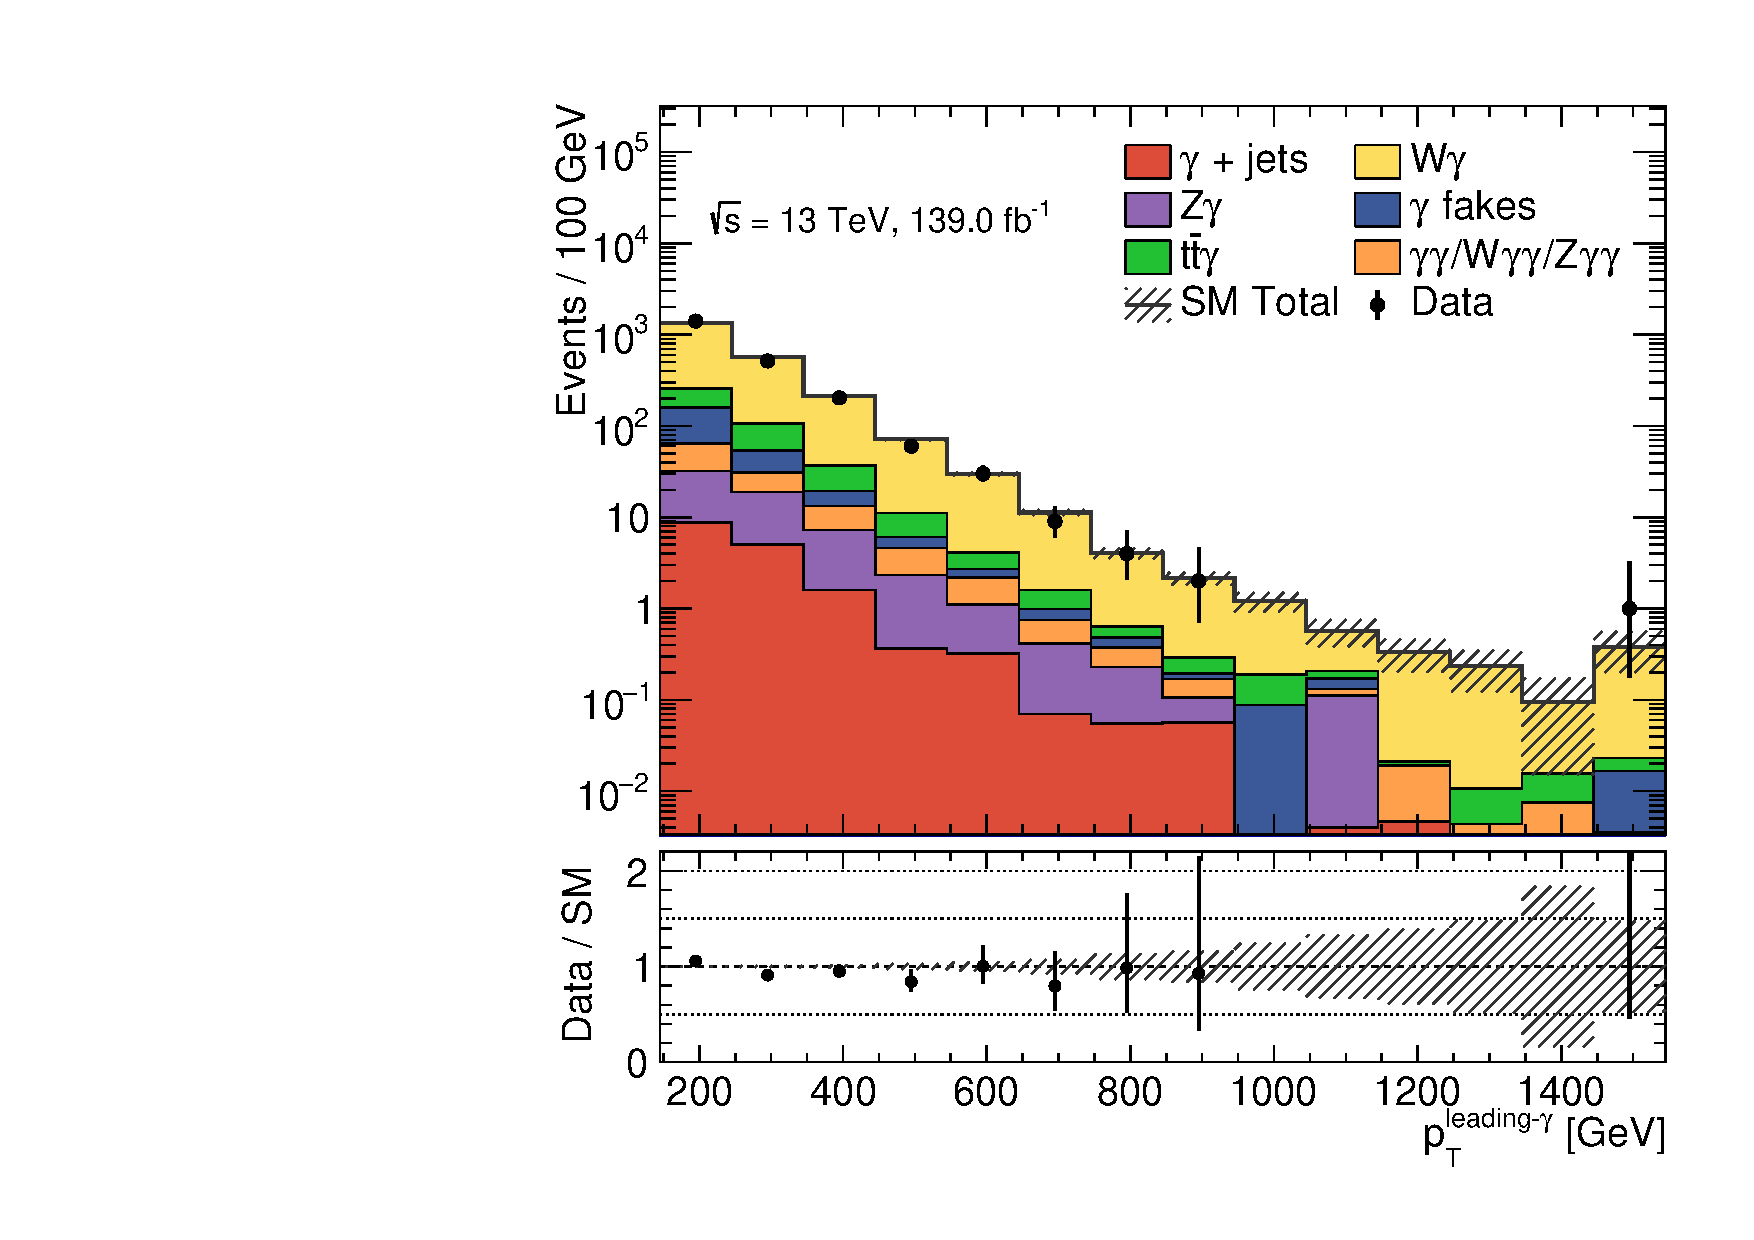
\includegraphics[width=0.32\textwidth]{images/results/fr2_unblind/can_CRW_ph_pt0_afterFit.pdf}
    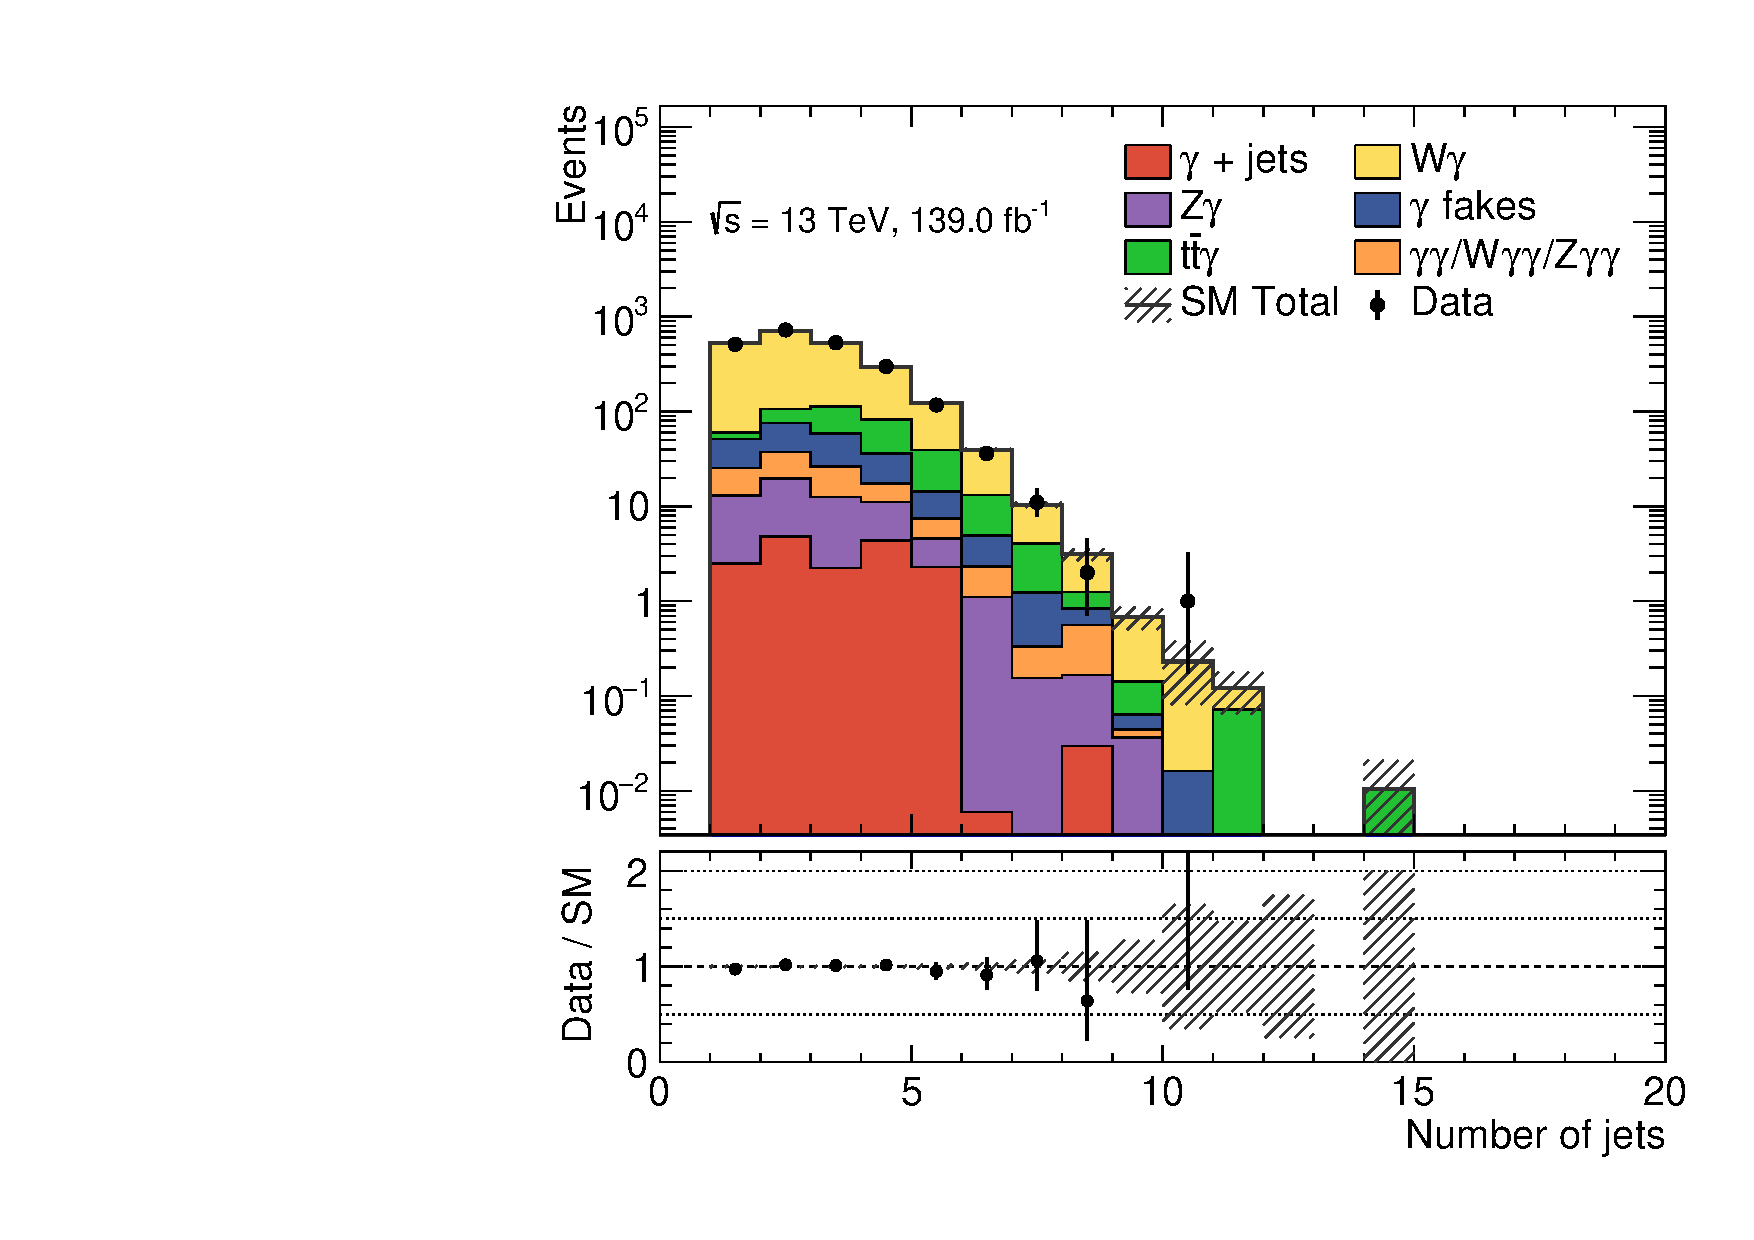
\includegraphics[width=0.32\textwidth]{images/results/fr2_unblind/can_CRW_jet_n_afterFit.pdf}
    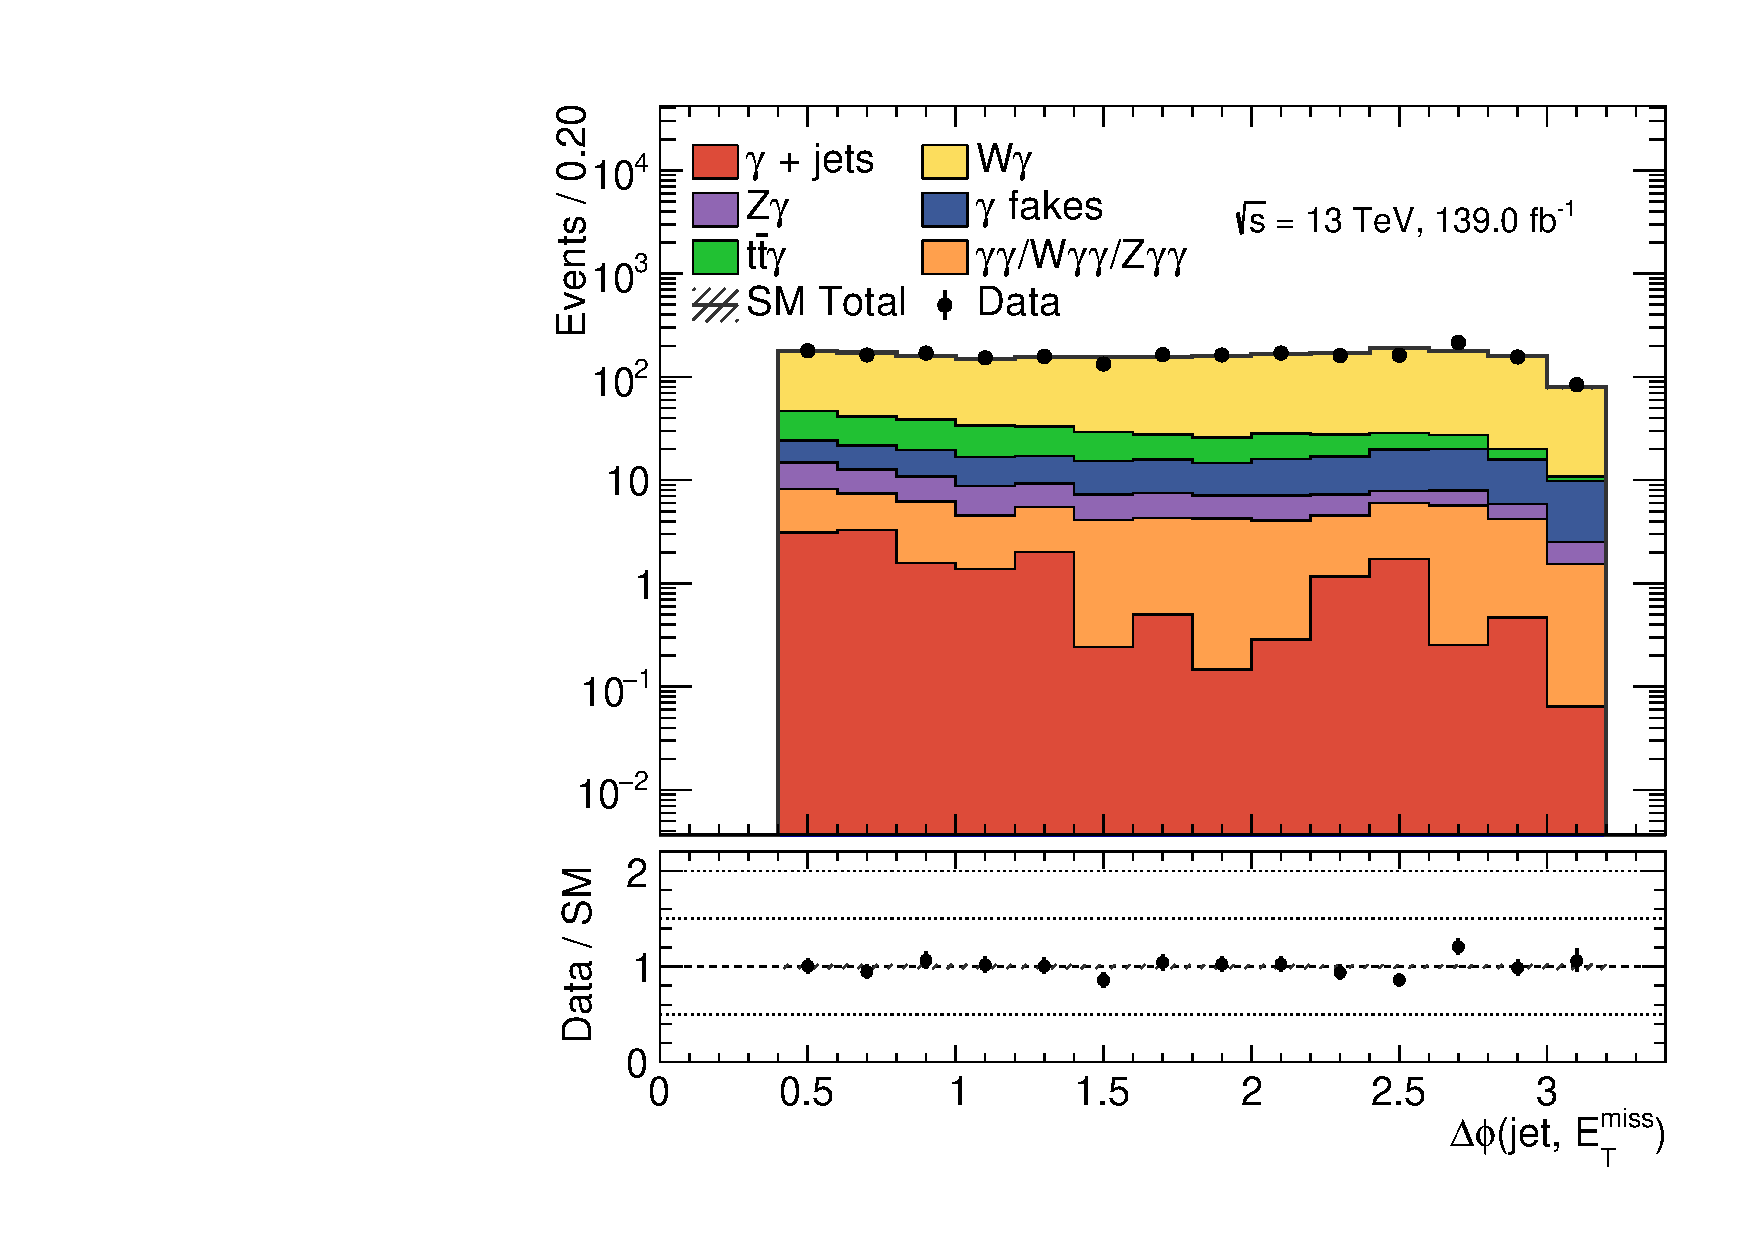
\includegraphics[width=0.32\textwidth]{images/results/fr2_unblind/can_CRW_dphi_jetmet_afterFit.pdf}

    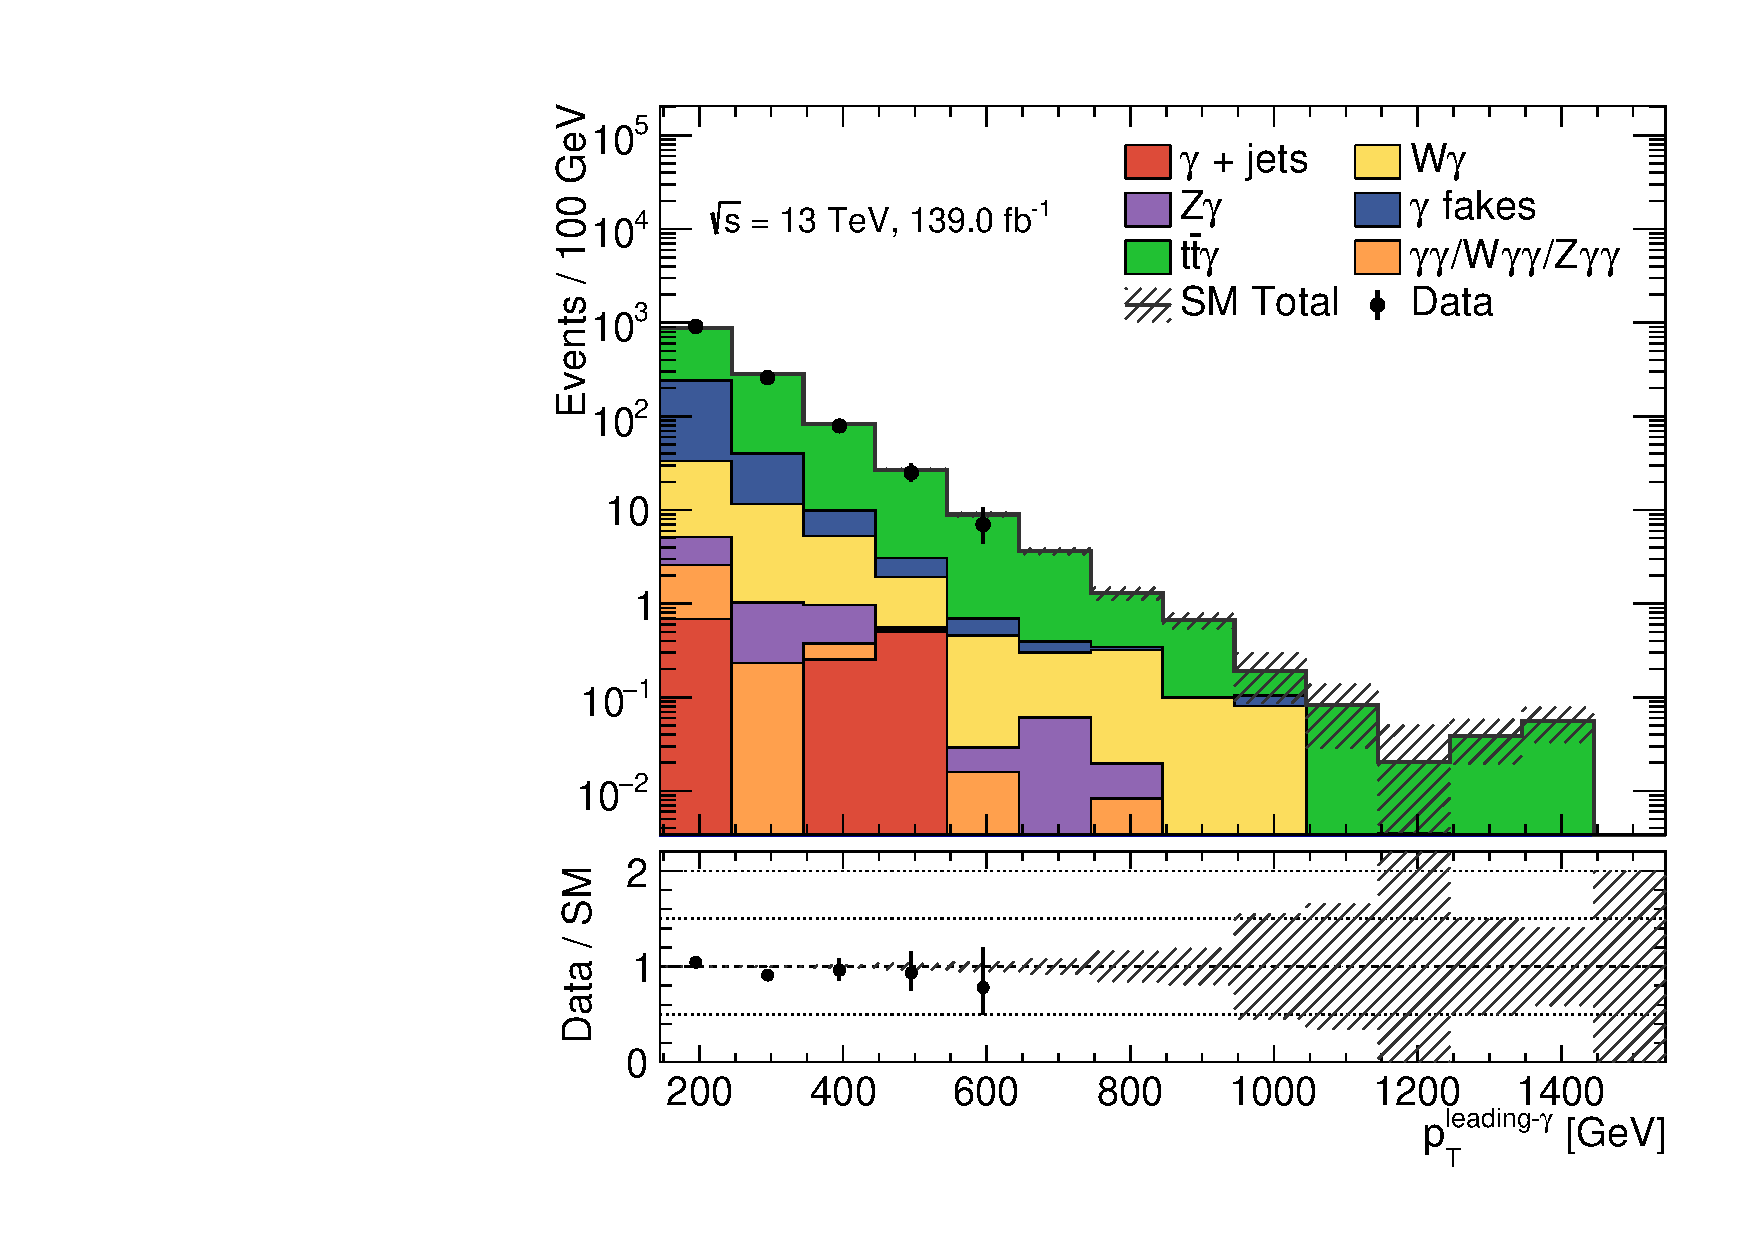
\includegraphics[width=0.32\textwidth]{images/results/fr2_unblind/can_CRT_ph_pt0_afterFit.pdf}
    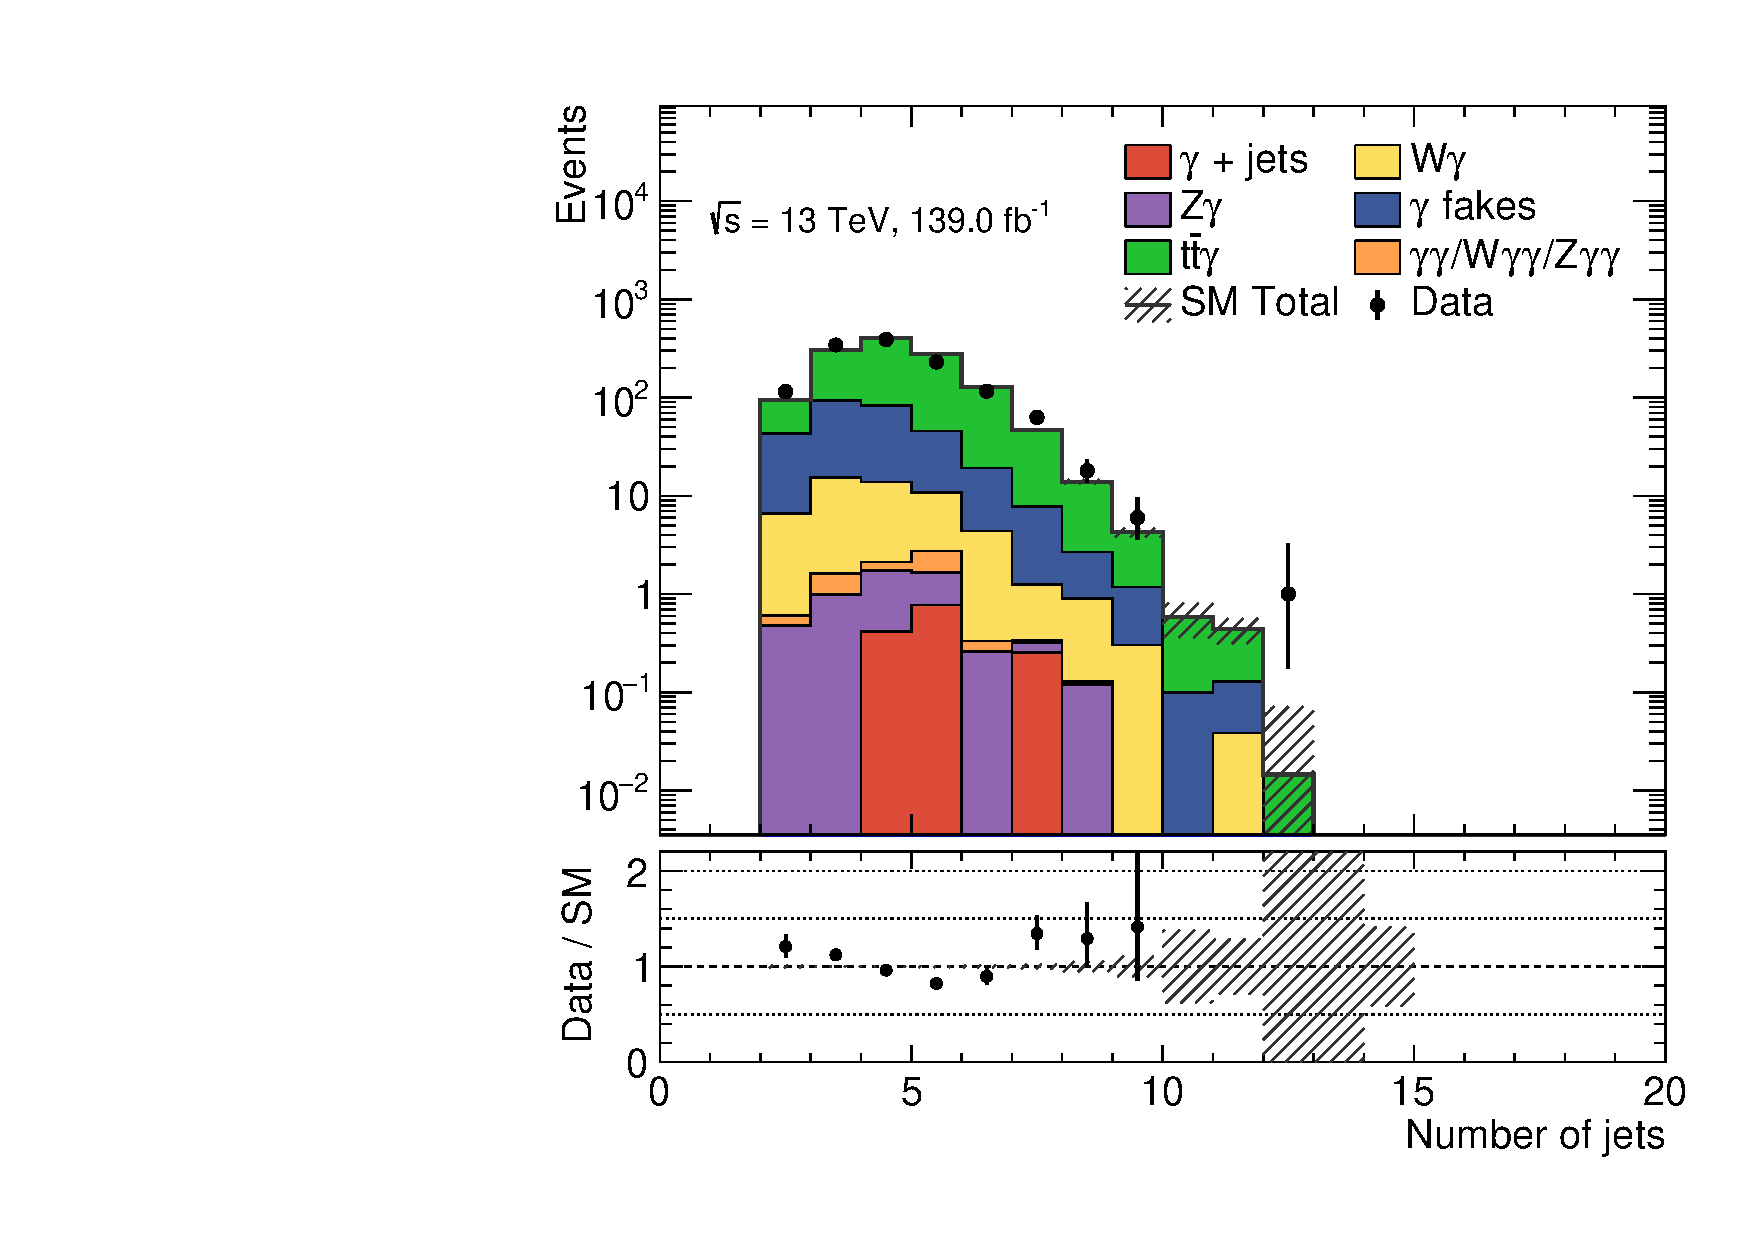
\includegraphics[width=0.32\textwidth]{images/results/fr2_unblind/can_CRT_jet_n_afterFit.pdf}
    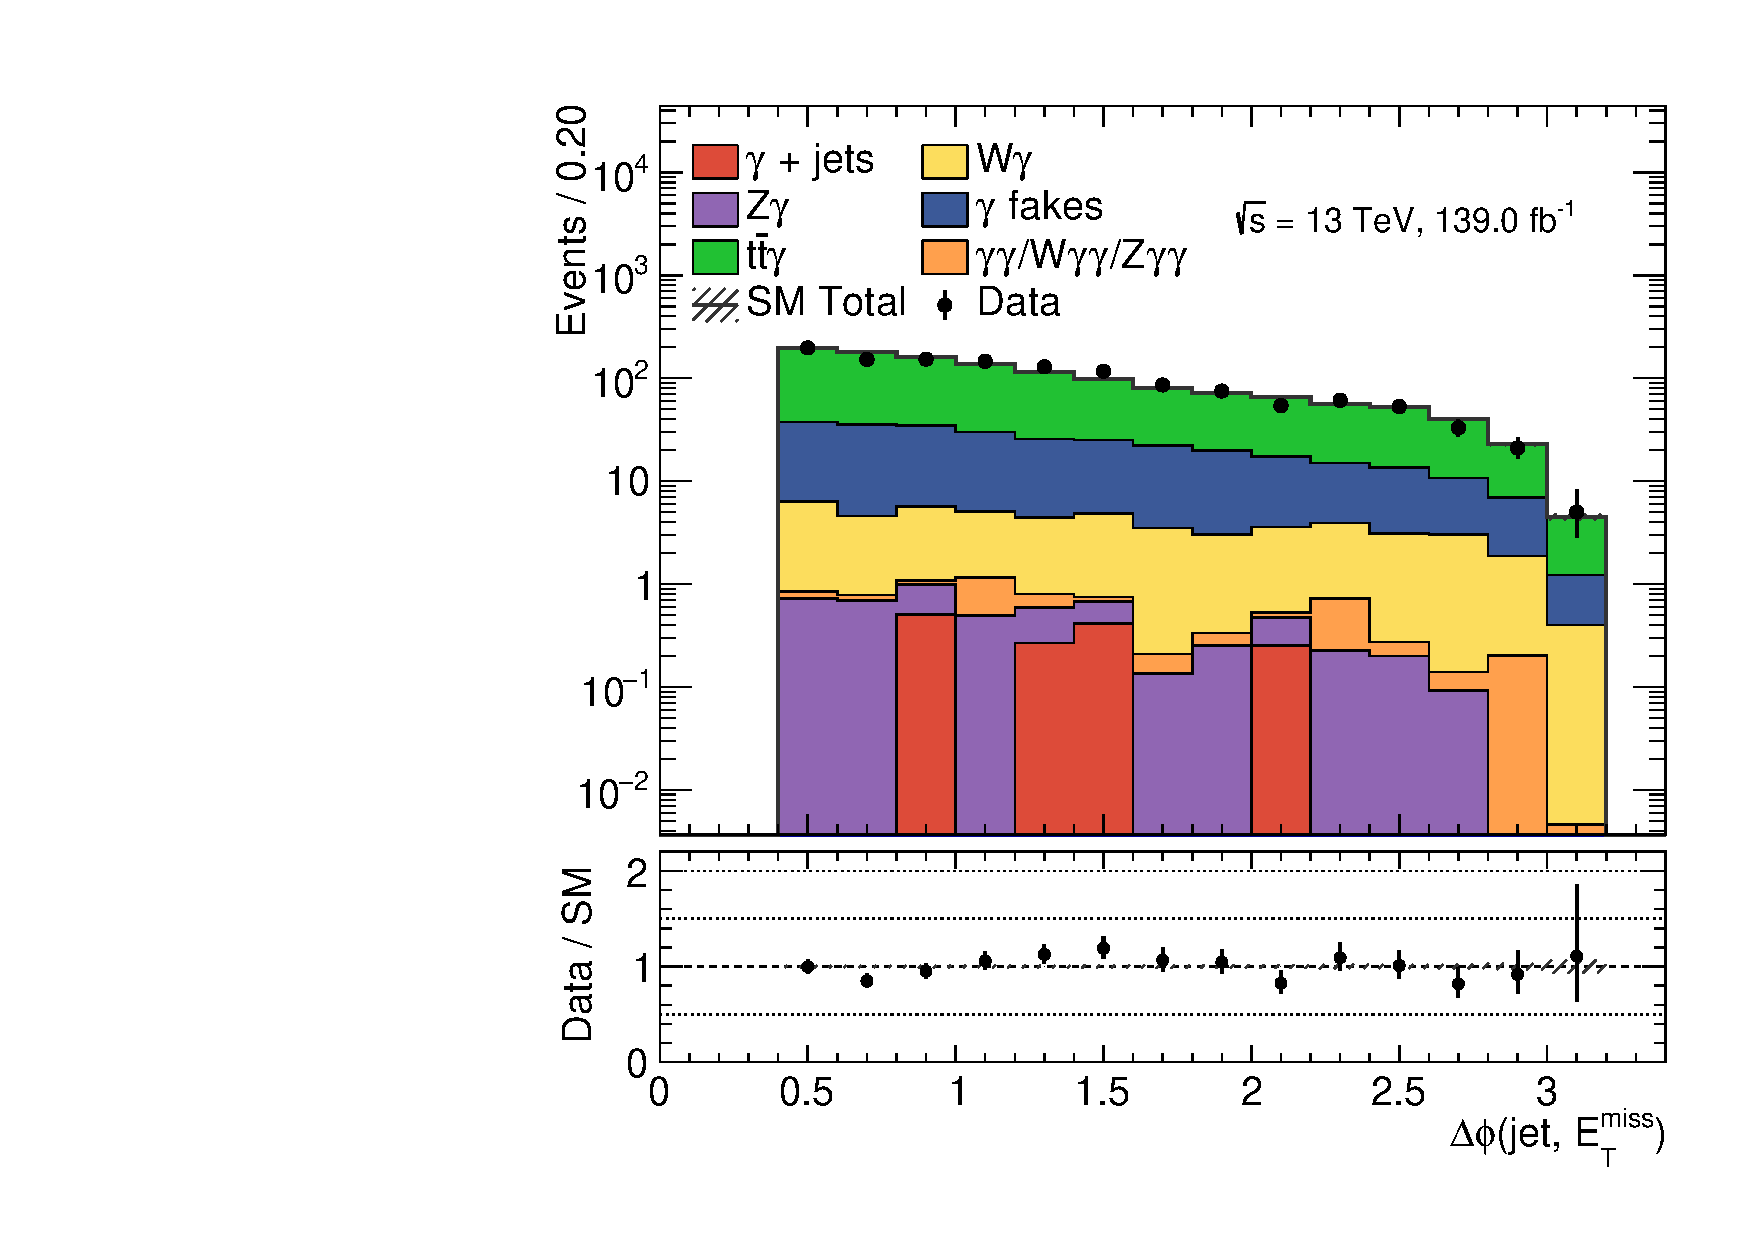
\includegraphics[width=0.32\textwidth]{images/results/fr2_unblind/can_CRT_dphi_jetmet_afterFit.pdf}

    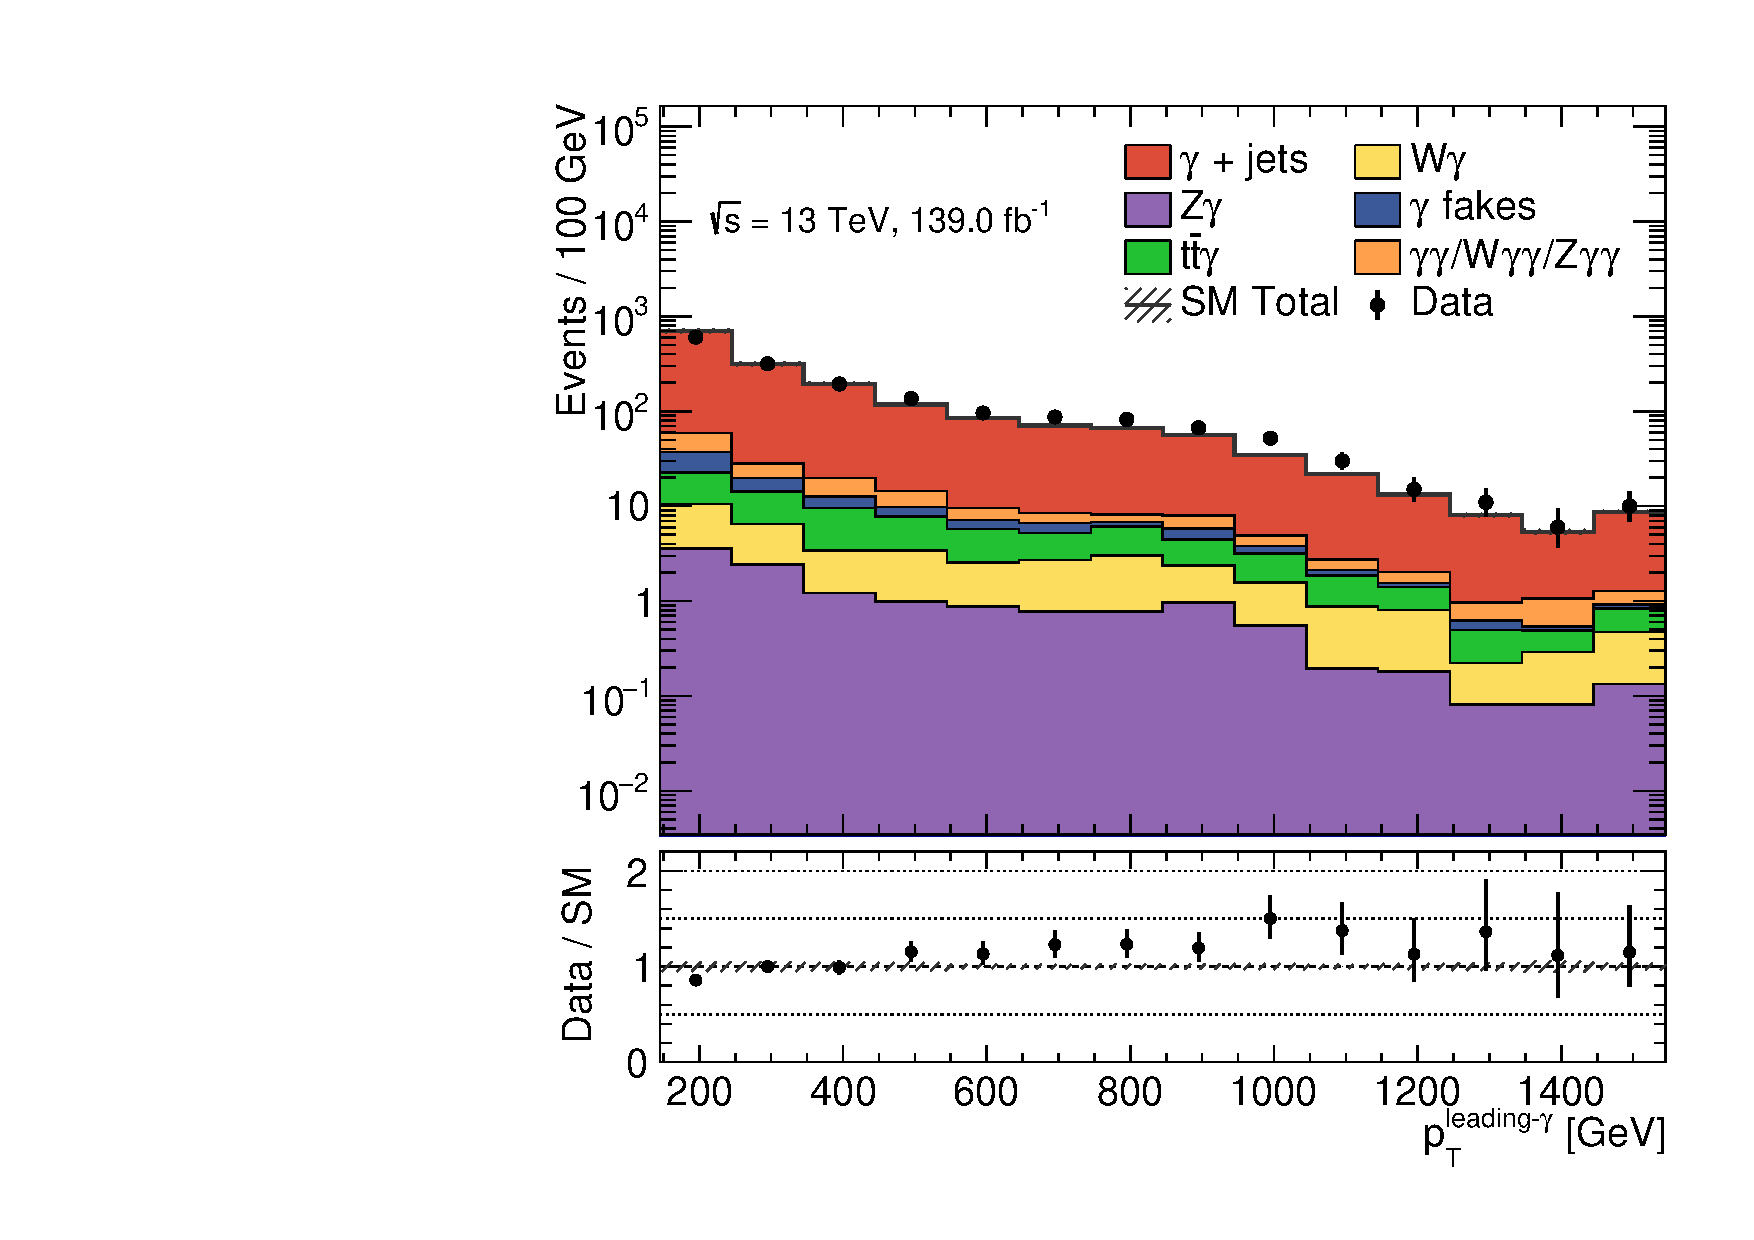
\includegraphics[width=0.32\textwidth]{images/results/fr2_unblind/can_CRQ_ph_pt0_afterFit.pdf}
    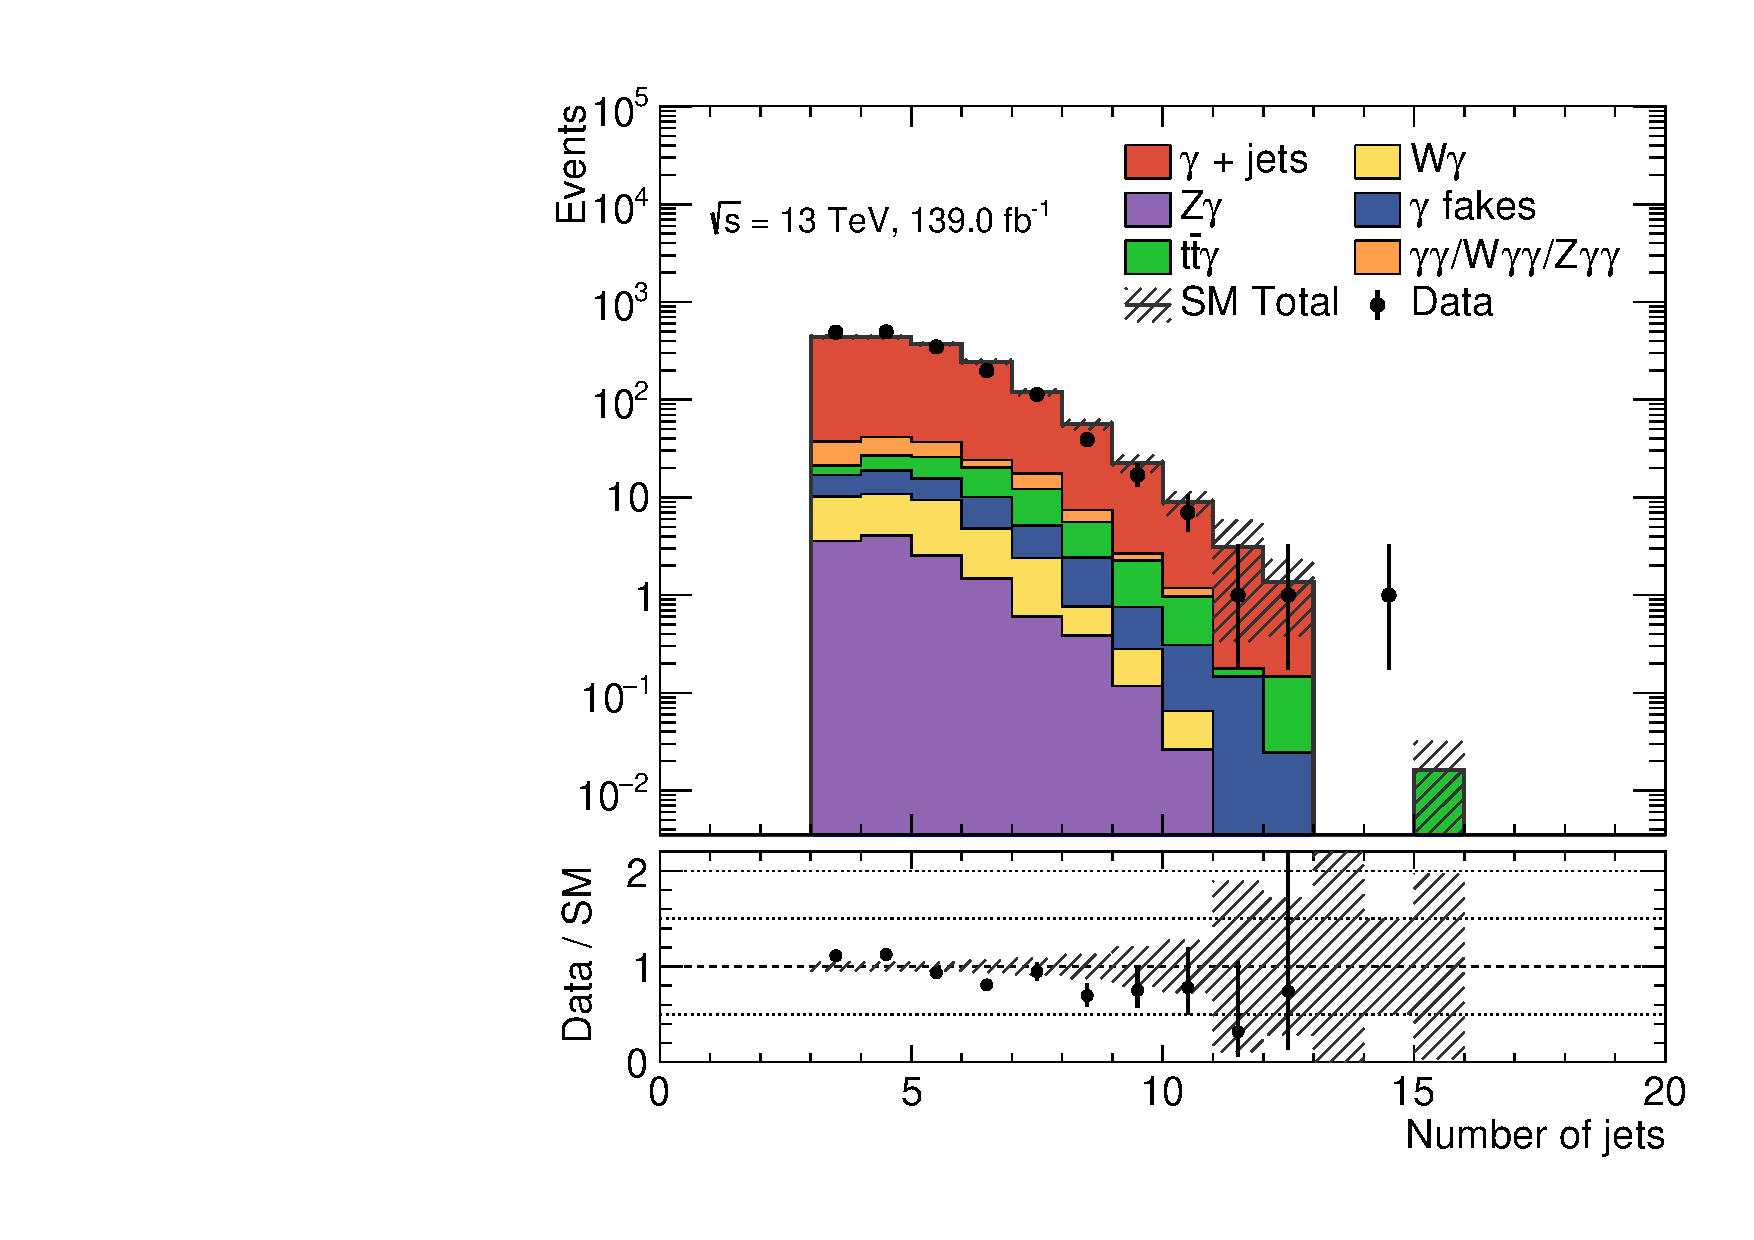
\includegraphics[width=0.32\textwidth]{images/results/fr2_unblind/can_CRQ_jet_n_afterFit.pdf}
    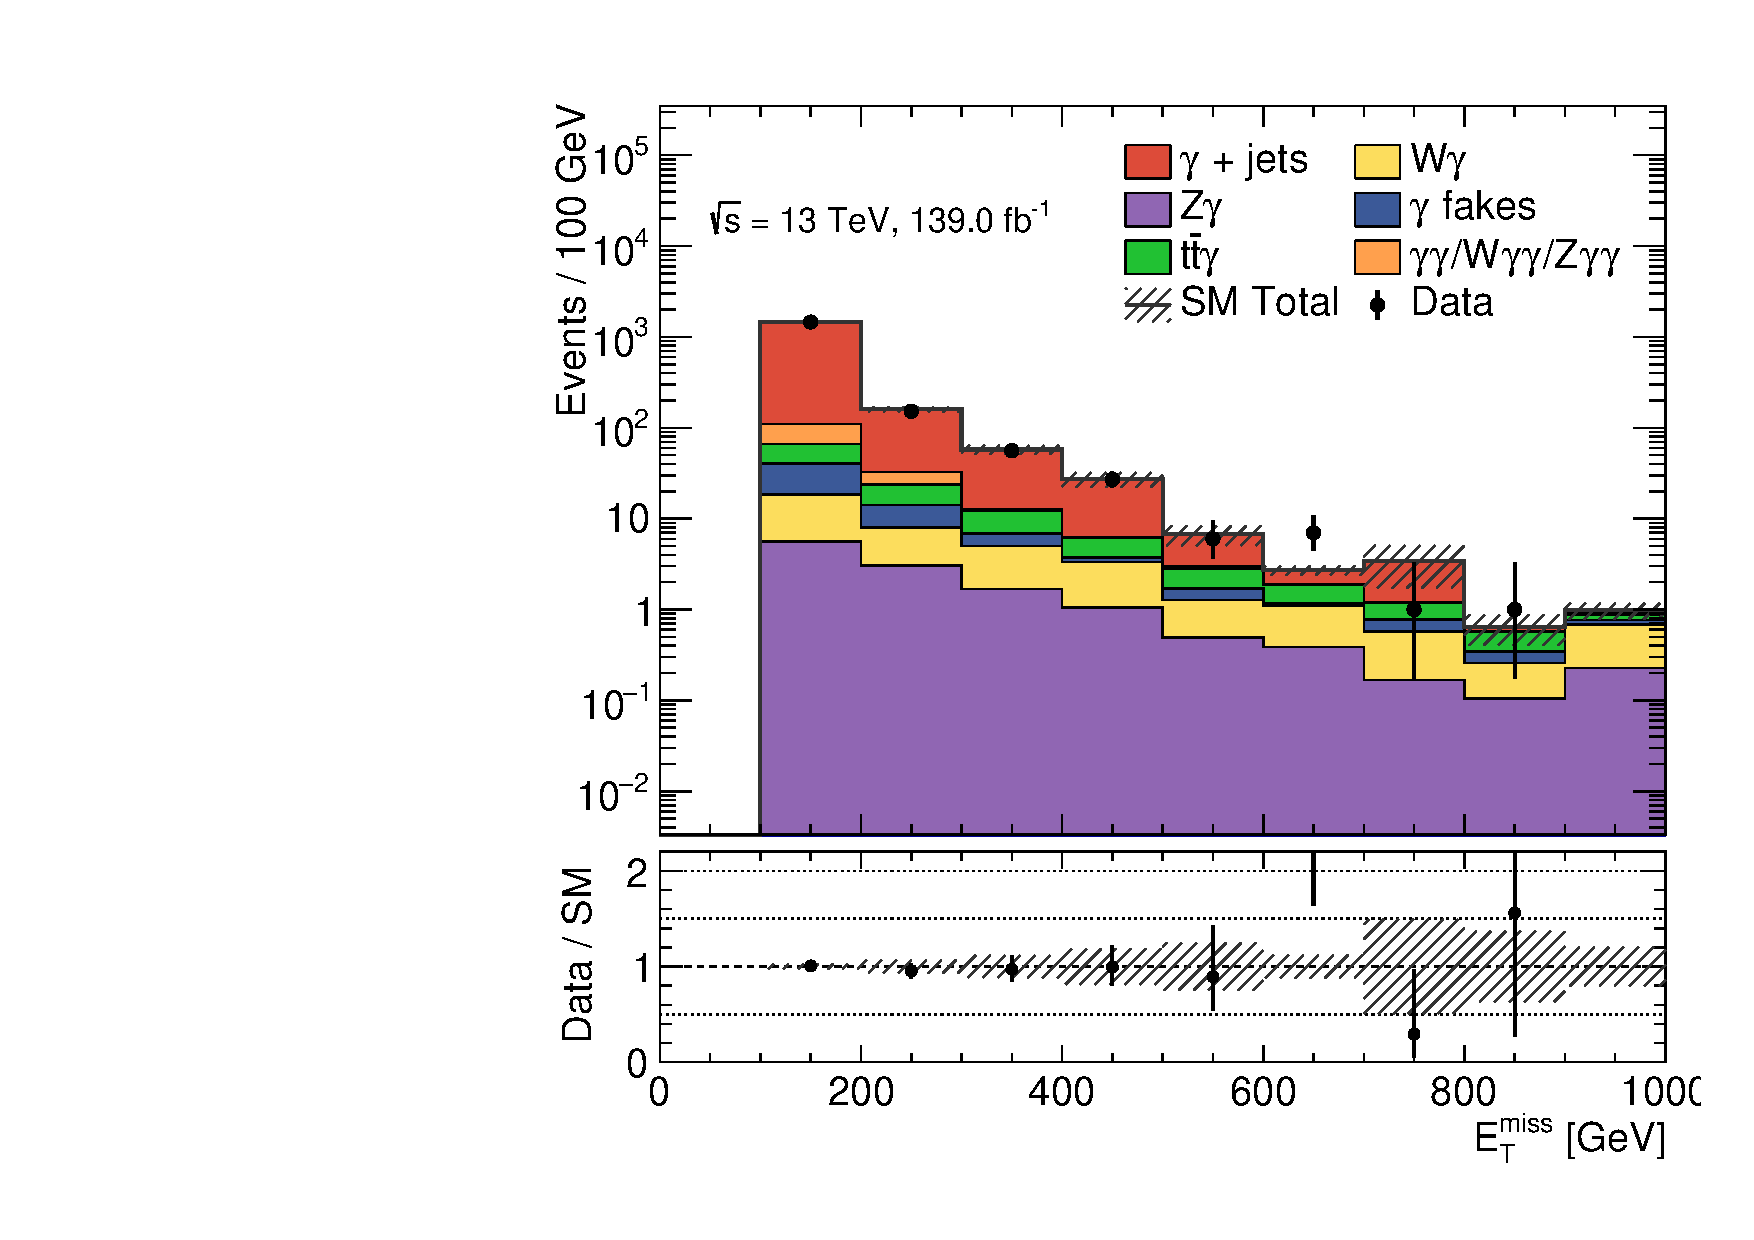
\includegraphics[width=0.32\textwidth]{images/results/fr2_unblind/can_CRQ_met_et_afterFit.pdf}

    \caption{Distribuciones de algunas variables significativas en las regiones de control CRW (arriba), CRT (medio) y CRQ (abajo) luego del ajuste de solo fondo. Las incertezas mostradas son sólo estadísticas.}
    \label{fig:cr_dist}
  \end{center}
\end{figure}



\begin{figure}[ht!]

  \centering
  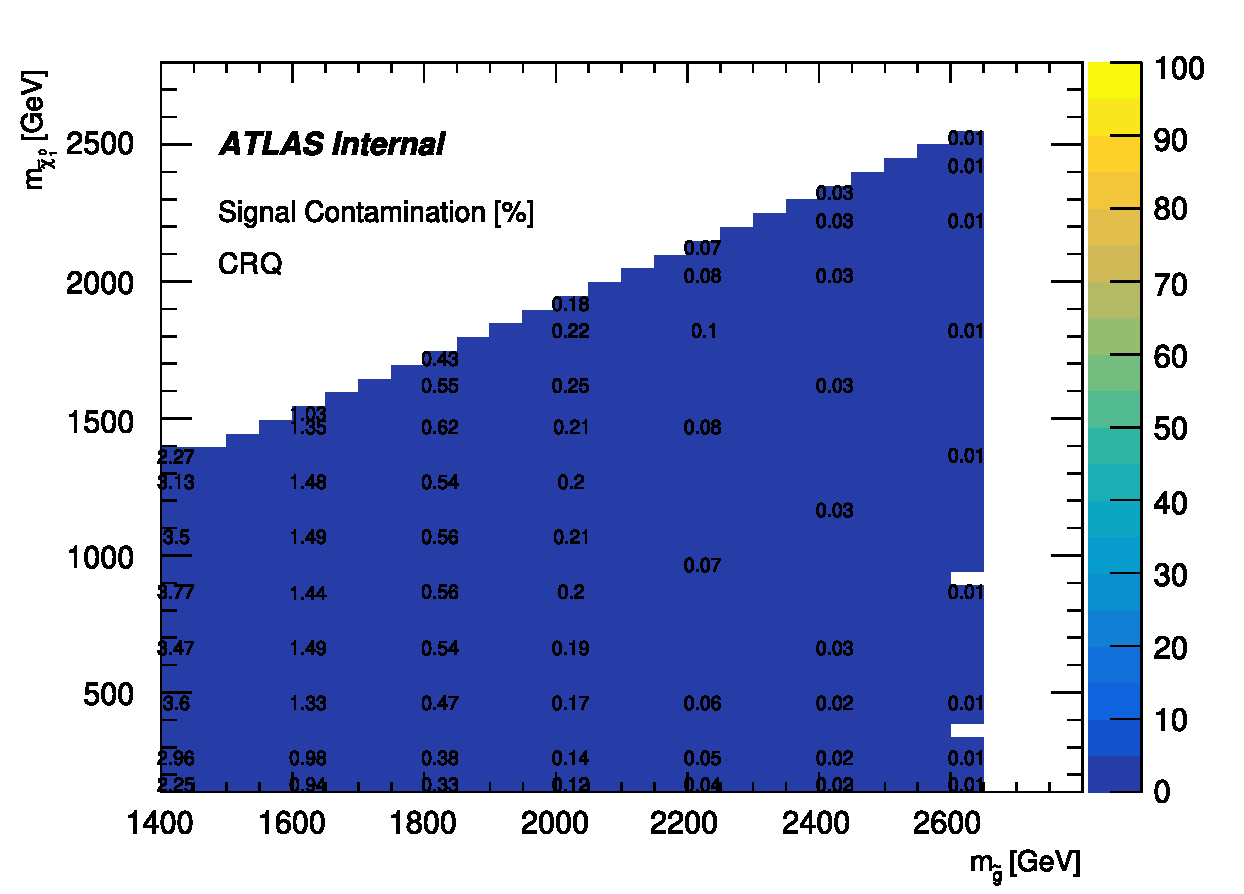
\includegraphics[width=0.32\textwidth]{images/results/signal_contamination_bb_CRQ_139ifb.pdf}
  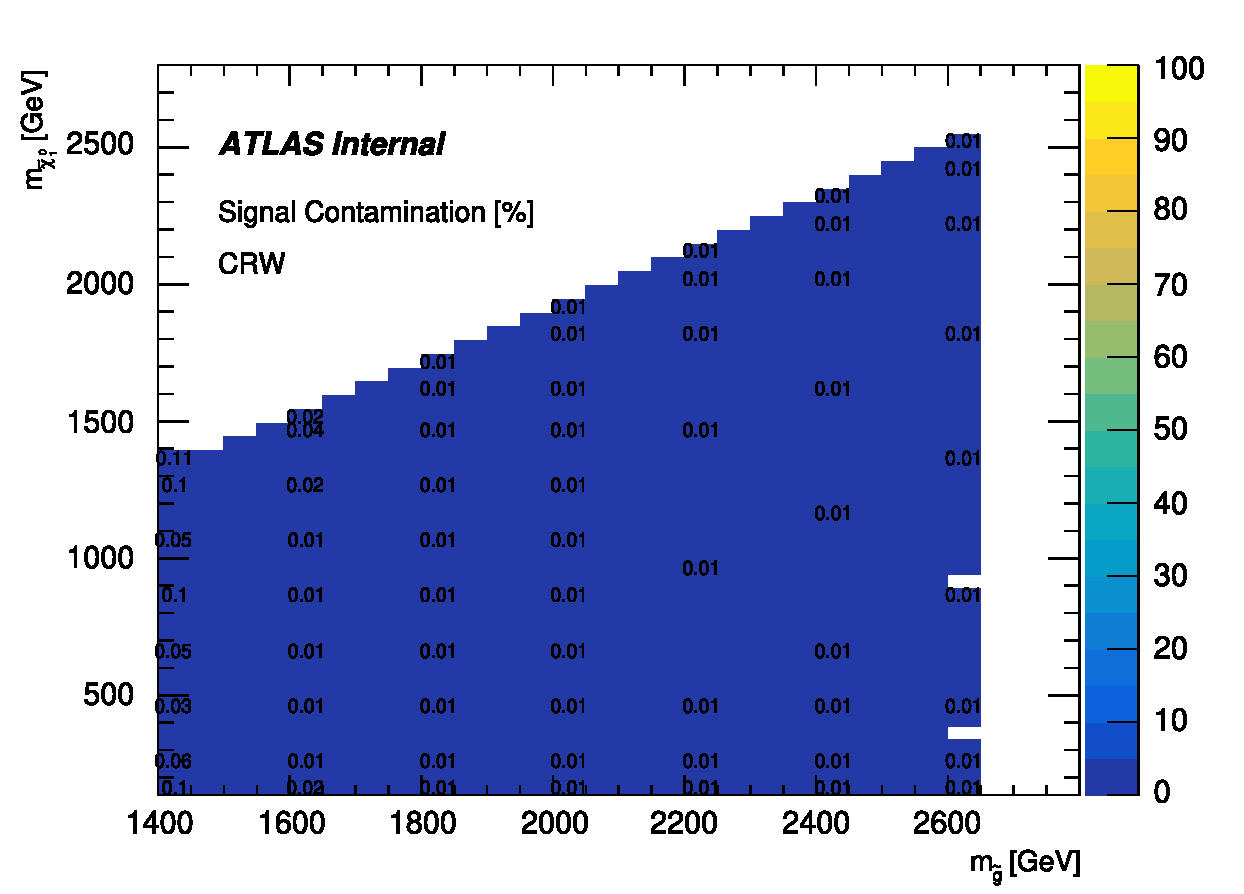
\includegraphics[width=0.32\textwidth]{images/results/signal_contamination_bb_CRW_139ifb.pdf}
  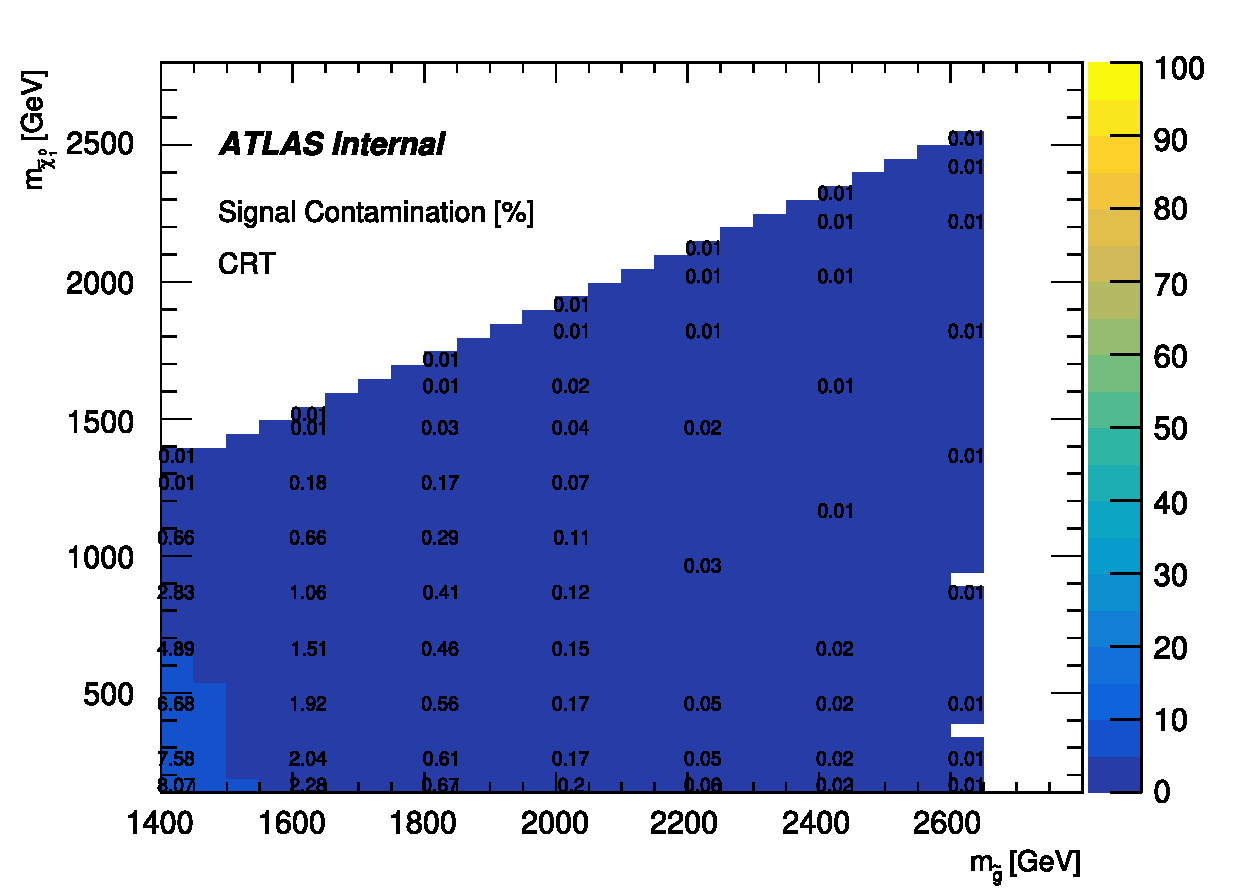
\includegraphics[width=0.32\textwidth]{images/results/signal_contamination_bb_CRT_139ifb.pdf}
  \caption{Contaminación porcentual para cada muestra de señal en las regiones de control CRQ (arriba izquierda), CRW (arriba derecha) y CRT (abajo). La misma se define como la fracción de eventos de señal con respecto al número de eventos de señal más fondo.}
  \label{fig:signal_contamination_CR_bb}

\end{figure}


En las Tablas \ref{tab:bkgonly_result_vrm}, \ref{tab:bkgonly_result_vrm} y \ref{tab:bkgonly_result_vre} se muestran los resultados de la estimación de los fondo en cada región de validación, y algunas de las distribuciones observadas en las mismas se muestran en las Figuras \ref{fig:dist_vrqm_bkgonly} y \ref{fig:dist_vrle_bkgonly}. Se encuentra un buen acuerdo entre los fondos y los datos observados para todas las regiones de validación, dando a entender que la estimación realizada es precisa, y permitiendo continuar con el siguiente paso, donde se comparan los datos observados y las predicciones en las regiones de señal. 


\begin{table}[ht!]
  \centering
  \caption{Estimación de los distintos fondos luego del ajuste de solo fondo en las regiones de validación VRQ, VRM1L, VRM2L, VRM1H y VRM2H.}
  \resizebox{\textwidth}{!}{\begin{tabular}{lrrrrr}
\hline
VRM & VRQ & VRM1L & VRM2L & VRM1H & VRM2H \\
\hline
Observed events & 714 & 127 & 22 & 419 & 51 \\
\hline
Expected SM events & $694.72 \pm 65.58$ & $134.08 \pm 15.99$ & $20.18 \pm 5.01$ & $385.06 \pm 37.21$ & $50.36 \pm 6.53$ \\
\hline
$e\rightarrow\gamma$ fakes & $15.97 \pm 1.17$ & $3.74 \pm 0.38$ & $1.30 \pm 0.19$ & $5.21 \pm 0.48$ & $1.37 \pm 0.20$ \\
$j\rightarrow\gamma$ fakes & $18.04 \pm 3.08$ & $3.59 \pm 0.69$ & $0.35 \pm 0.11$ & $10.38 \pm 1.77$ & $1.28 \pm 0.26$ \\
$\gamma$ + jets & $573.52 \pm 64.46$ & $109.86 \pm 15.13$ & $14.12 \pm 4.26$ & $313.65 \pm 36.88$ & $31.34 \pm 6.10$ \\
$W\gamma$ & $26.99 \pm 1.95$ & $3.67 \pm 0.44$ & $1.11 \pm 0.35$ & $18.59 \pm 1.24$ & $6.79 \pm 0.86$ \\
$Z(\rightarrow\ell\ell)\gamma$ & $2.09 \pm 0.60$ & $0.29 \pm 0.11$ & $0.14 \pm 0.07$ & $1.09 \pm 0.35$ & $0.28 \pm 0.17$ \\
$Z(\rightarrow\nu\nu)\gamma$ & $9.65 \pm 2.67$ & $0.89 \pm 0.26$ & $0.45 \pm 0.16$ & $5.94 \pm 1.64$ & $2.63 \pm 0.75$ \\
$t\bar{t}\gamma$ & $23.91 \pm 1.80$ & $9.80 \pm 1.02$ & $2.34 \pm 0.57$ & $15.70 \pm 1.17$ & $4.39 \pm 0.51$ \\
$\gamma\gamma / W\gamma\gamma / Z\gamma\gamma$ & $24.55 \pm 1.97$ & $2.23 \pm 0.77$ & $0.37 \pm 0.12$ & $14.50 \pm 1.32$ & $2.29 \pm 0.42$ \\
\hline
\end{tabular}
}
  %\resizebox{\textwidth}{!}{\begin{tabular}{lrrrrr}
\hline
VRM & VRQ & VRM1L & VRM2L & VRM1H & VRM2H \\
\hline
Observed events & 714 & 127 & 22 & 419 & 51 \\
\hline
Expected SM events & $694.72 \pm 65.58$ & $134.08 \pm 15.99$ & $20.18 \pm 5.01$ & $385.06 \pm 37.21$ & $50.36 \pm 6.53$ \\
\hline
$e\rightarrow\gamma$ fakes & $15.97 \pm 1.17$ & $3.74 \pm 0.38$ & $1.30 \pm 0.19$ & $5.21 \pm 0.48$ & $1.37 \pm 0.20$ \\
$j\rightarrow\gamma$ fakes & $18.04 \pm 3.08$ & $3.59 \pm 0.69$ & $0.35 \pm 0.11$ & $10.38 \pm 1.77$ & $1.28 \pm 0.26$ \\
$\gamma$ + jets & $573.52 \pm 64.46$ & $109.86 \pm 15.13$ & $14.12 \pm 4.26$ & $313.65 \pm 36.88$ & $31.34 \pm 6.10$ \\
$W\gamma$ & $26.99 \pm 1.95$ & $3.67 \pm 0.44$ & $1.11 \pm 0.35$ & $18.59 \pm 1.24$ & $6.79 \pm 0.86$ \\
$Z(\rightarrow\ell\ell)\gamma$ & $2.09 \pm 0.60$ & $0.29 \pm 0.11$ & $0.14 \pm 0.07$ & $1.09 \pm 0.35$ & $0.28 \pm 0.17$ \\
$Z(\rightarrow\nu\nu)\gamma$ & $9.65 \pm 2.67$ & $0.89 \pm 0.26$ & $0.45 \pm 0.16$ & $5.94 \pm 1.64$ & $2.63 \pm 0.75$ \\
$t\bar{t}\gamma$ & $23.91 \pm 1.80$ & $9.80 \pm 1.02$ & $2.34 \pm 0.57$ & $15.70 \pm 1.17$ & $4.39 \pm 0.51$ \\
$\gamma\gamma / W\gamma\gamma / Z\gamma\gamma$ & $24.55 \pm 1.97$ & $2.23 \pm 0.77$ & $0.37 \pm 0.12$ & $14.50 \pm 1.32$ & $2.29 \pm 0.42$ \\
\hline
\end{tabular}
}
  \label{tab:bkgonly_result_vrm}
\end{table}


\begin{table}[ht!]
  \centering
  \caption{Estimación de los distintos fondos luego del ajuste de solo fondo en las regiones de validación VRL1, VRL2, VRL3 y VRL4.}
  \resizebox{\textwidth}{!}{\begin{tabular}{lrrrr}
\hline
VRL & VRL1 & VRL2 & VRL3 & VRL4 \\
\hline
Observed events & 1731 & 257 & 699 & 52 \\
\hline
Expected SM events & $1686.63 \pm 48.08$ & $252.19 \pm 11.37$ & $734.90 \pm 23.54$ & $51.54 \pm 2.88$ \\
\hline
$e\rightarrow\gamma$ fakes & $151.56 \pm 9.46$ & $20.50 \pm 1.45$ & $51.82 \pm 3.38$ & $4.48 \pm 0.44$ \\
$j\rightarrow\gamma$ fakes & $32.36 \pm 4.88$ & $3.67 \pm 0.62$ & $25.84 \pm 9.28$ & $1.08 \pm 0.38$ \\
$\gamma$ + jets & $21.85 \pm 6.65$ & $4.75 \pm 1.14$ & $1.81 \pm 0.57$ & $0.15_{-0.15}^{+0.16}$ \\
$W\gamma$ & $877.59 \pm 44.21$ & $144.49 \pm 9.04$ & $430.59 \pm 22.23$ & $17.23 \pm 1.52$ \\
$Z(\rightarrow\ell\ell)\gamma$ & $52.81 \pm 14.45$ & $10.62 \pm 3.00$ & $7.39 \pm 2.01$ & $0.74 \pm 0.25$ \\
$Z(\rightarrow\nu\nu)\gamma$ & $0.03 \pm 0.01$ & $0.01 \pm 0.00$ & $0.03 \pm 0.01$ & $0.00 \pm 0.00$ \\
$t\bar{t}\gamma$ & $510.48 \pm 27.74$ & $59.19 \pm 3.62$ & $203.73 \pm 11.06$ & $26.91 \pm 1.97$ \\
$\gamma\gamma / W\gamma\gamma / Z\gamma\gamma$ & $39.95 \pm 1.73$ & $8.96 \pm 0.70$ & $13.70 \pm 0.61$ & $0.95 \pm 0.06$ \\
\hline
\end{tabular}
}
  %\resizebox{\textwidth}{!}{\begin{tabular}{lrrrr}
\hline
VRL & VRL1 & VRL2 & VRL3 & VRL4 \\
\hline
Observed events & 1731 & 257 & 699 & 52 \\
\hline
Expected SM events & $1686.63 \pm 48.08$ & $252.19 \pm 11.37$ & $734.90 \pm 23.54$ & $51.54 \pm 2.88$ \\
\hline
$e\rightarrow\gamma$ fakes & $151.56 \pm 9.46$ & $20.50 \pm 1.45$ & $51.82 \pm 3.38$ & $4.48 \pm 0.44$ \\
$j\rightarrow\gamma$ fakes & $32.36 \pm 4.88$ & $3.67 \pm 0.62$ & $25.84 \pm 9.28$ & $1.08 \pm 0.38$ \\
$\gamma$ + jets & $21.85 \pm 6.65$ & $4.75 \pm 1.14$ & $1.81 \pm 0.57$ & $0.15_{-0.15}^{+0.16}$ \\
$W\gamma$ & $877.59 \pm 44.21$ & $144.49 \pm 9.04$ & $430.59 \pm 22.23$ & $17.23 \pm 1.52$ \\
$Z(\rightarrow\ell\ell)\gamma$ & $52.81 \pm 14.45$ & $10.62 \pm 3.00$ & $7.39 \pm 2.01$ & $0.74 \pm 0.25$ \\
$Z(\rightarrow\nu\nu)\gamma$ & $0.03 \pm 0.01$ & $0.01 \pm 0.00$ & $0.03 \pm 0.01$ & $0.00 \pm 0.00$ \\
$t\bar{t}\gamma$ & $510.48 \pm 27.74$ & $59.19 \pm 3.62$ & $203.73 \pm 11.06$ & $26.91 \pm 1.97$ \\
$\gamma\gamma / W\gamma\gamma / Z\gamma\gamma$ & $39.95 \pm 1.73$ & $8.96 \pm 0.70$ & $13.70 \pm 0.61$ & $0.95 \pm 0.06$ \\
\hline
\end{tabular}
}
  \label{tab:bkgonly_result_vrl}
\end{table}

\begin{table}[ht!]
  \centering
  \caption{Estimación de los distintos fondos luego del ajuste de solo fondo en la VRE.}
  \begin{tabular}{lr}
\hline
Fakes VR & VRE \\
\hline
Observed events & 520 \\
\hline
Expected SM events & $550.63 \pm 31.61$ \\
\hline
$e\rightarrow\gamma$ fakes & $418.40 \pm 25.79$ \\
$j\rightarrow\gamma$ fakes & $46.25 \pm 15.98$ \\
$\gamma$ + jets & $7.59 \pm 2.06$ \\
$W\gamma$ & $48.36 \pm 7.79$ \\
$Z(\rightarrow\ell\ell)\gamma$ & $0.45 \pm 0.11$ \\
$Z(\rightarrow\nu\nu)\gamma$ & $4.54 \pm 1.15$ \\
$t\bar{t}\gamma$ & $23.10 \pm 2.37$ \\
$\gamma\gamma / W\gamma\gamma / Z\gamma\gamma$ & $1.95 \pm 0.30$ \\
\hline
\end{tabular}

  %\begin{tabular}{lr}
\hline
Fakes VR & VRE \\
\hline
Observed events & 520 \\
\hline
Expected SM events & $550.63 \pm 31.61$ \\
\hline
$e\rightarrow\gamma$ fakes & $418.40 \pm 25.79$ \\
$j\rightarrow\gamma$ fakes & $46.25 \pm 15.98$ \\
$\gamma$ + jets & $7.59 \pm 2.06$ \\
$W\gamma$ & $48.36 \pm 7.79$ \\
$Z(\rightarrow\ell\ell)\gamma$ & $0.45 \pm 0.11$ \\
$Z(\rightarrow\nu\nu)\gamma$ & $4.54 \pm 1.15$ \\
$t\bar{t}\gamma$ & $23.10 \pm 2.37$ \\
$\gamma\gamma / W\gamma\gamma / Z\gamma\gamma$ & $1.95 \pm 0.30$ \\
\hline
\end{tabular}

  \label{tab:bkgonly_result_vre}
\end{table}

\begin{figure}[ht!]
  \centering

    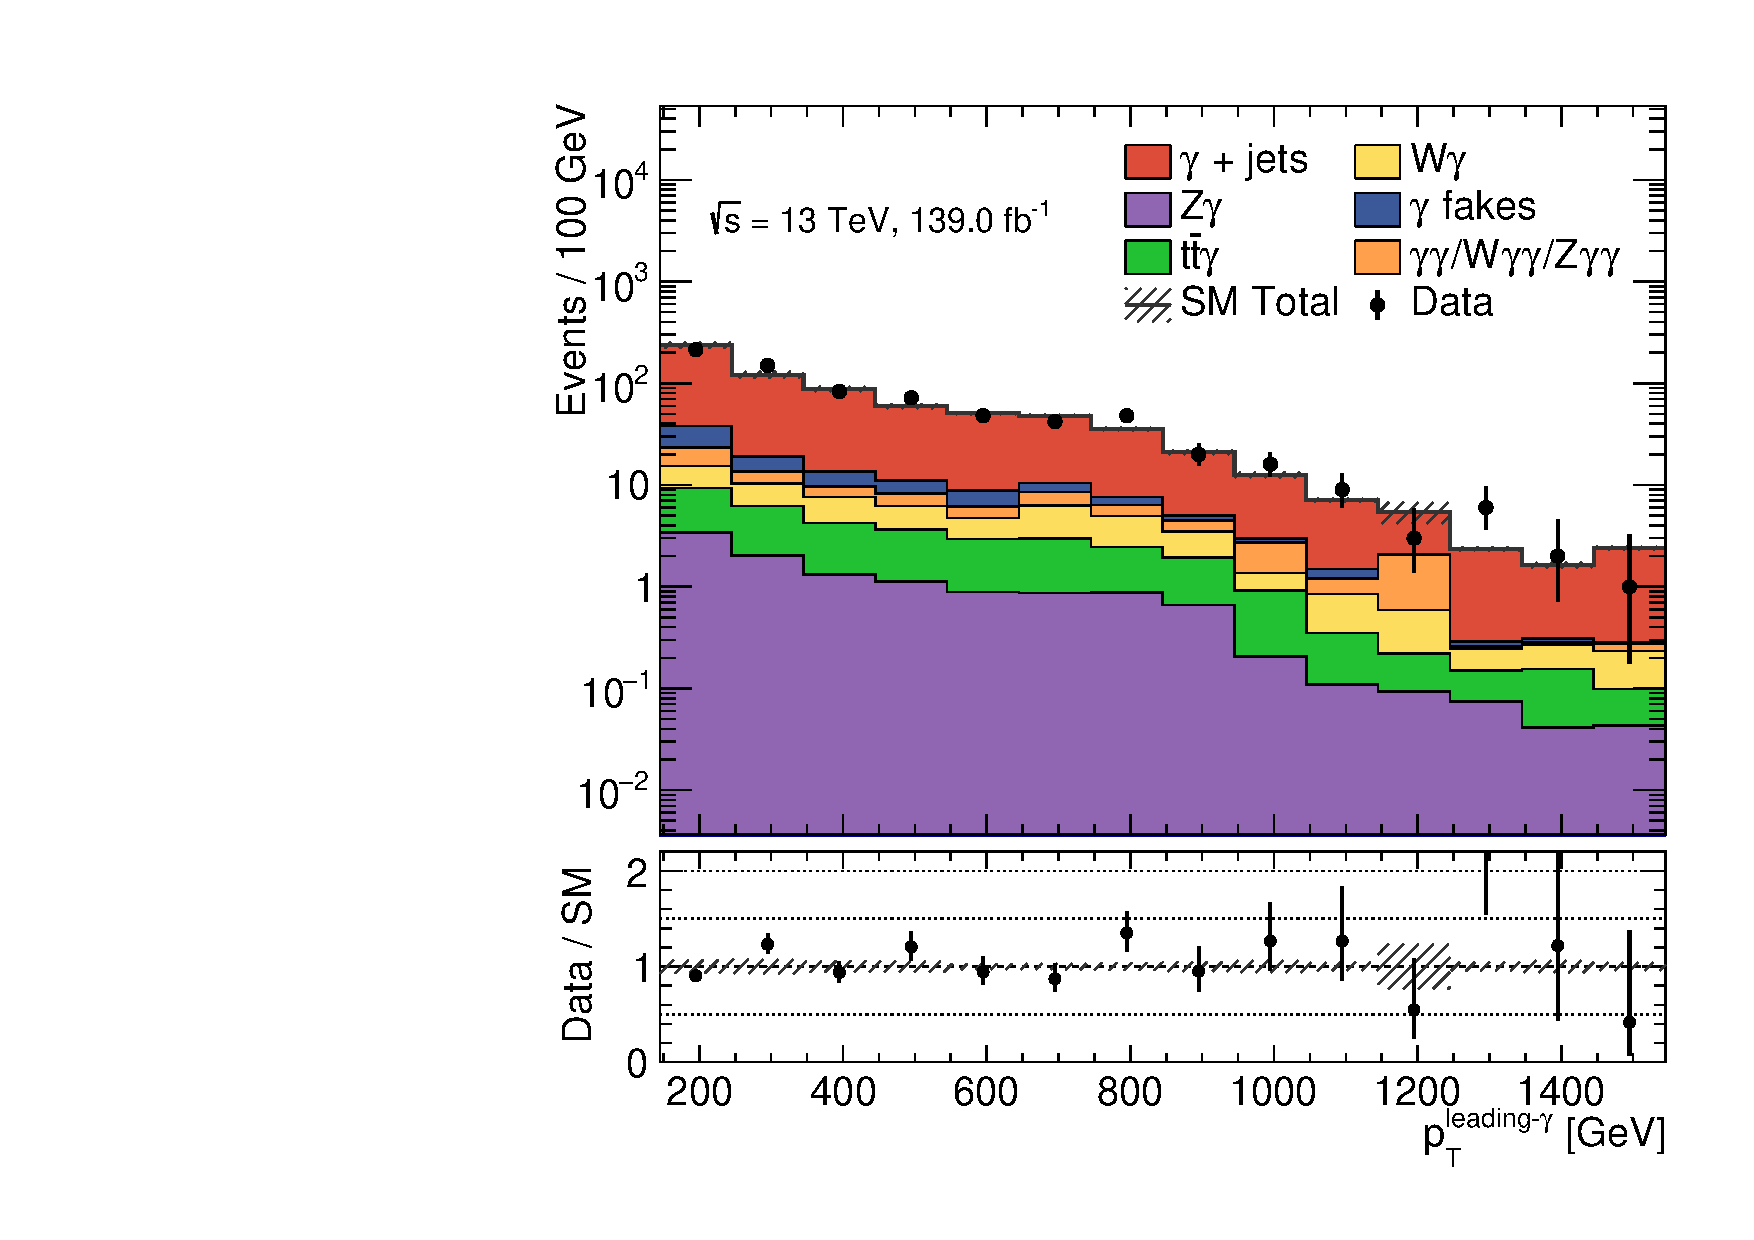
\includegraphics[width=0.32\textwidth]{images/results/fr2_unblind/can_VRQ_ph_pt0_afterFit.pdf}
    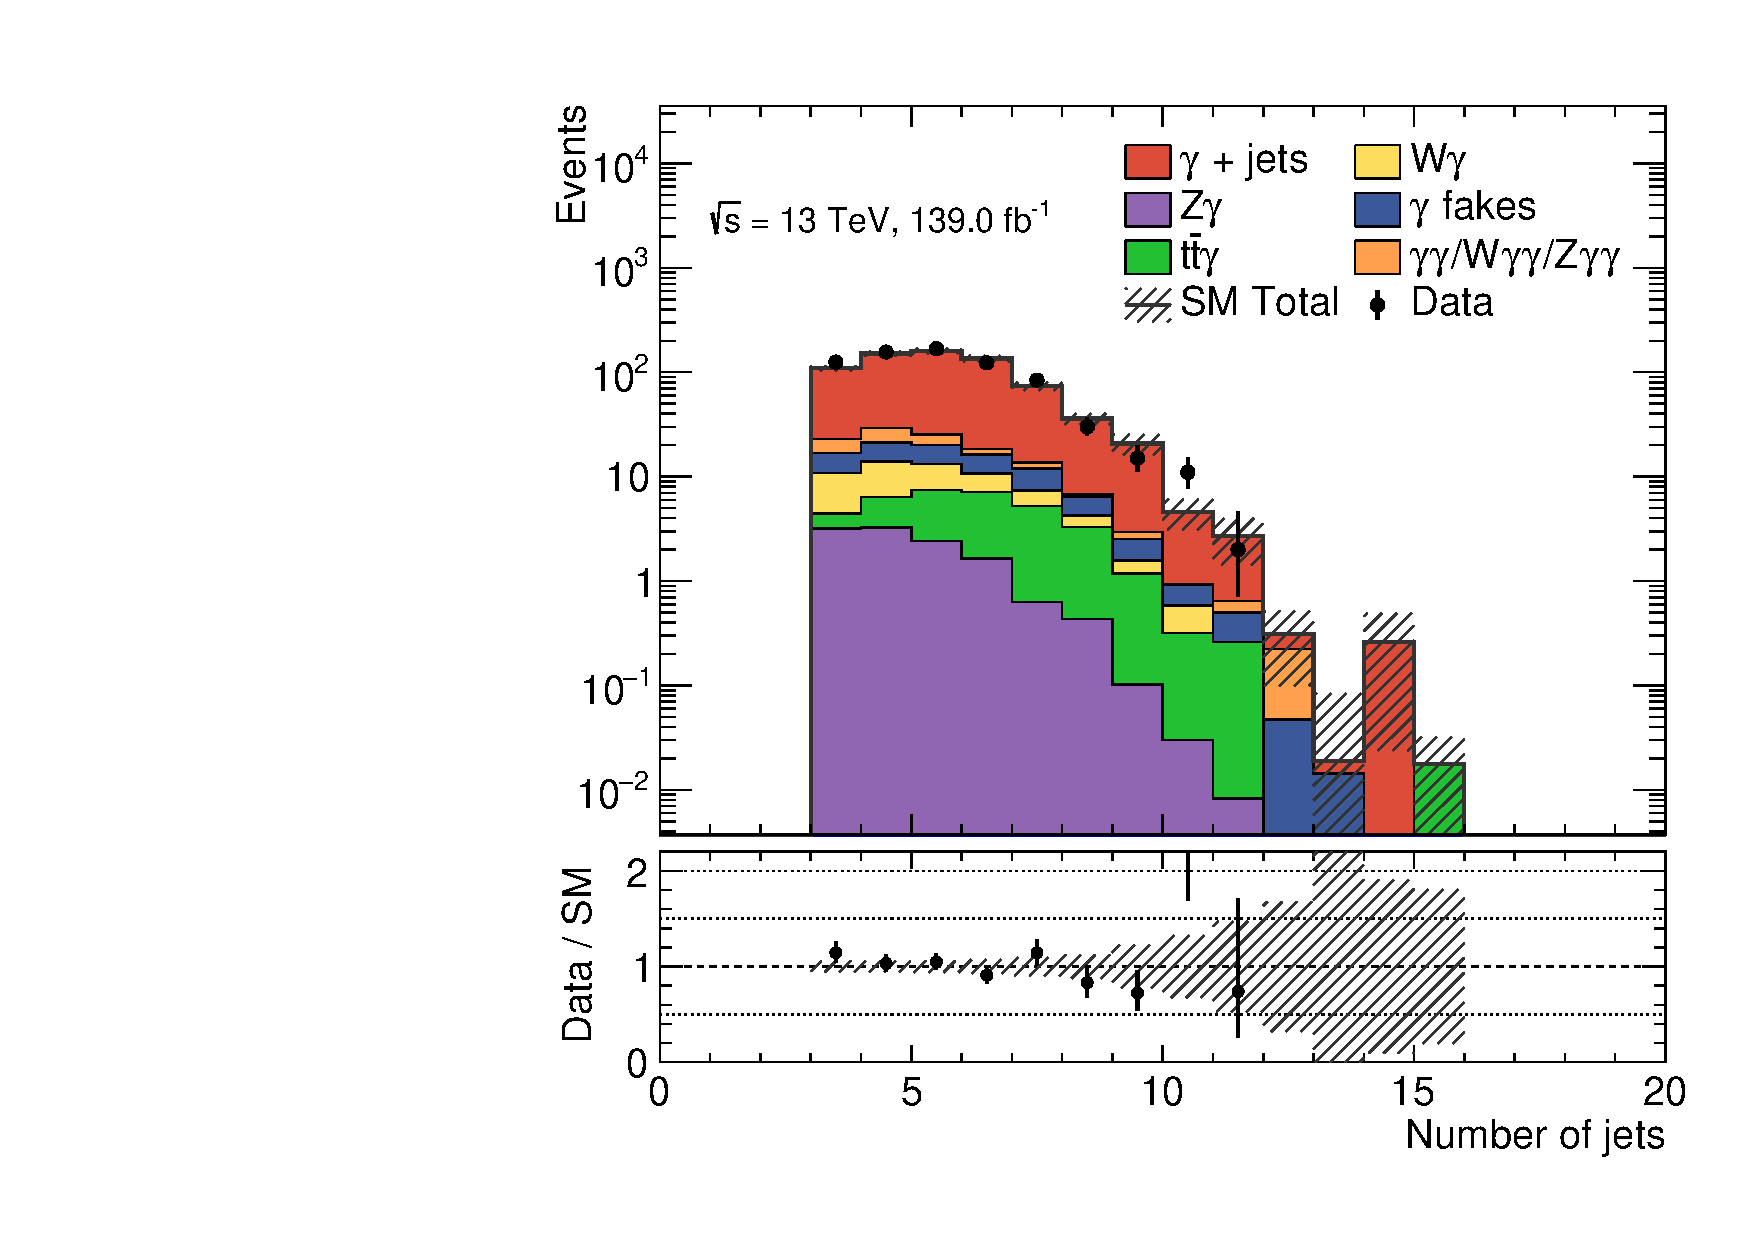
\includegraphics[width=0.32\textwidth]{images/results/fr2_unblind/can_VRQ_jet_n_afterFit.pdf}
    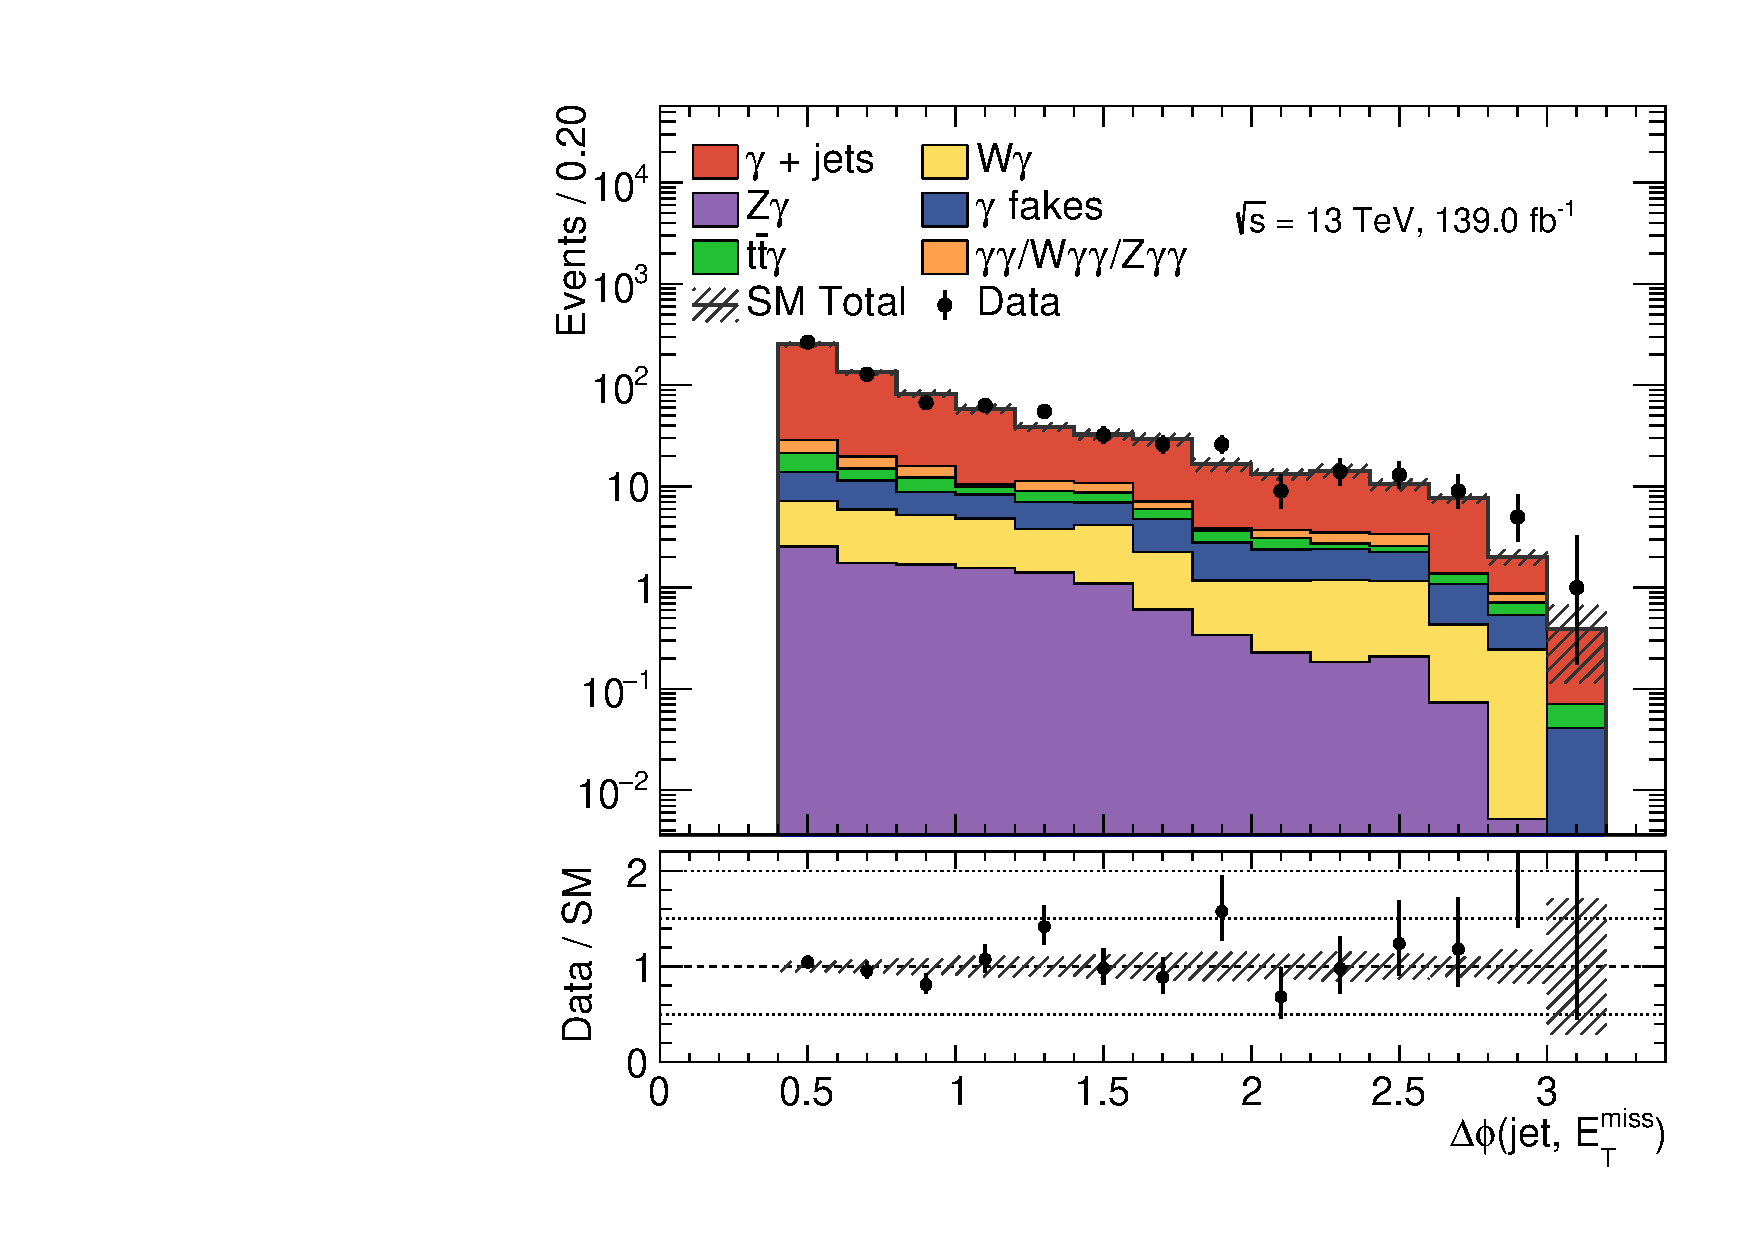
\includegraphics[width=0.32\textwidth]{images/results/fr2_unblind/can_VRQ_dphi_jetmet_afterFit.pdf}

    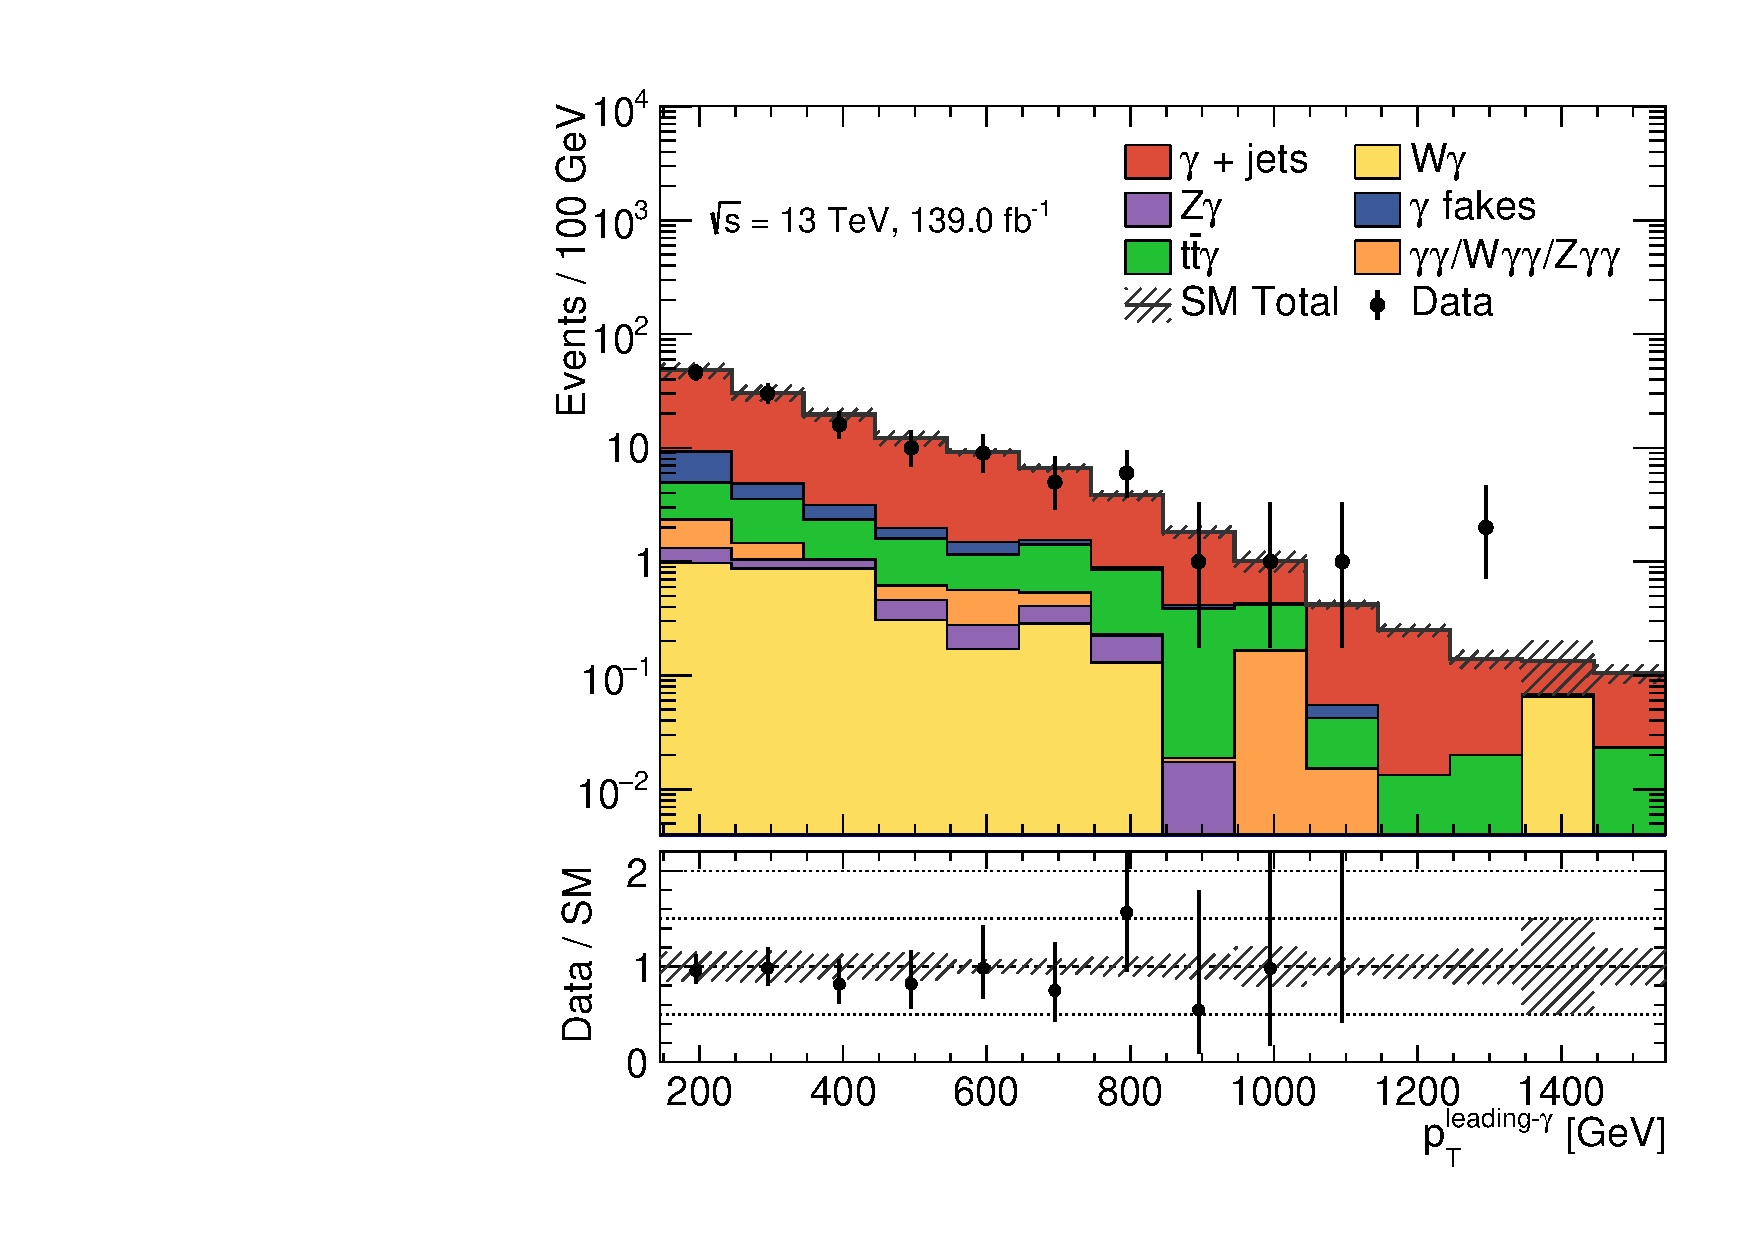
\includegraphics[width=0.32\textwidth]{images/results/fr2_unblind/can_VRM1L_ph_pt0_afterFit.pdf}
    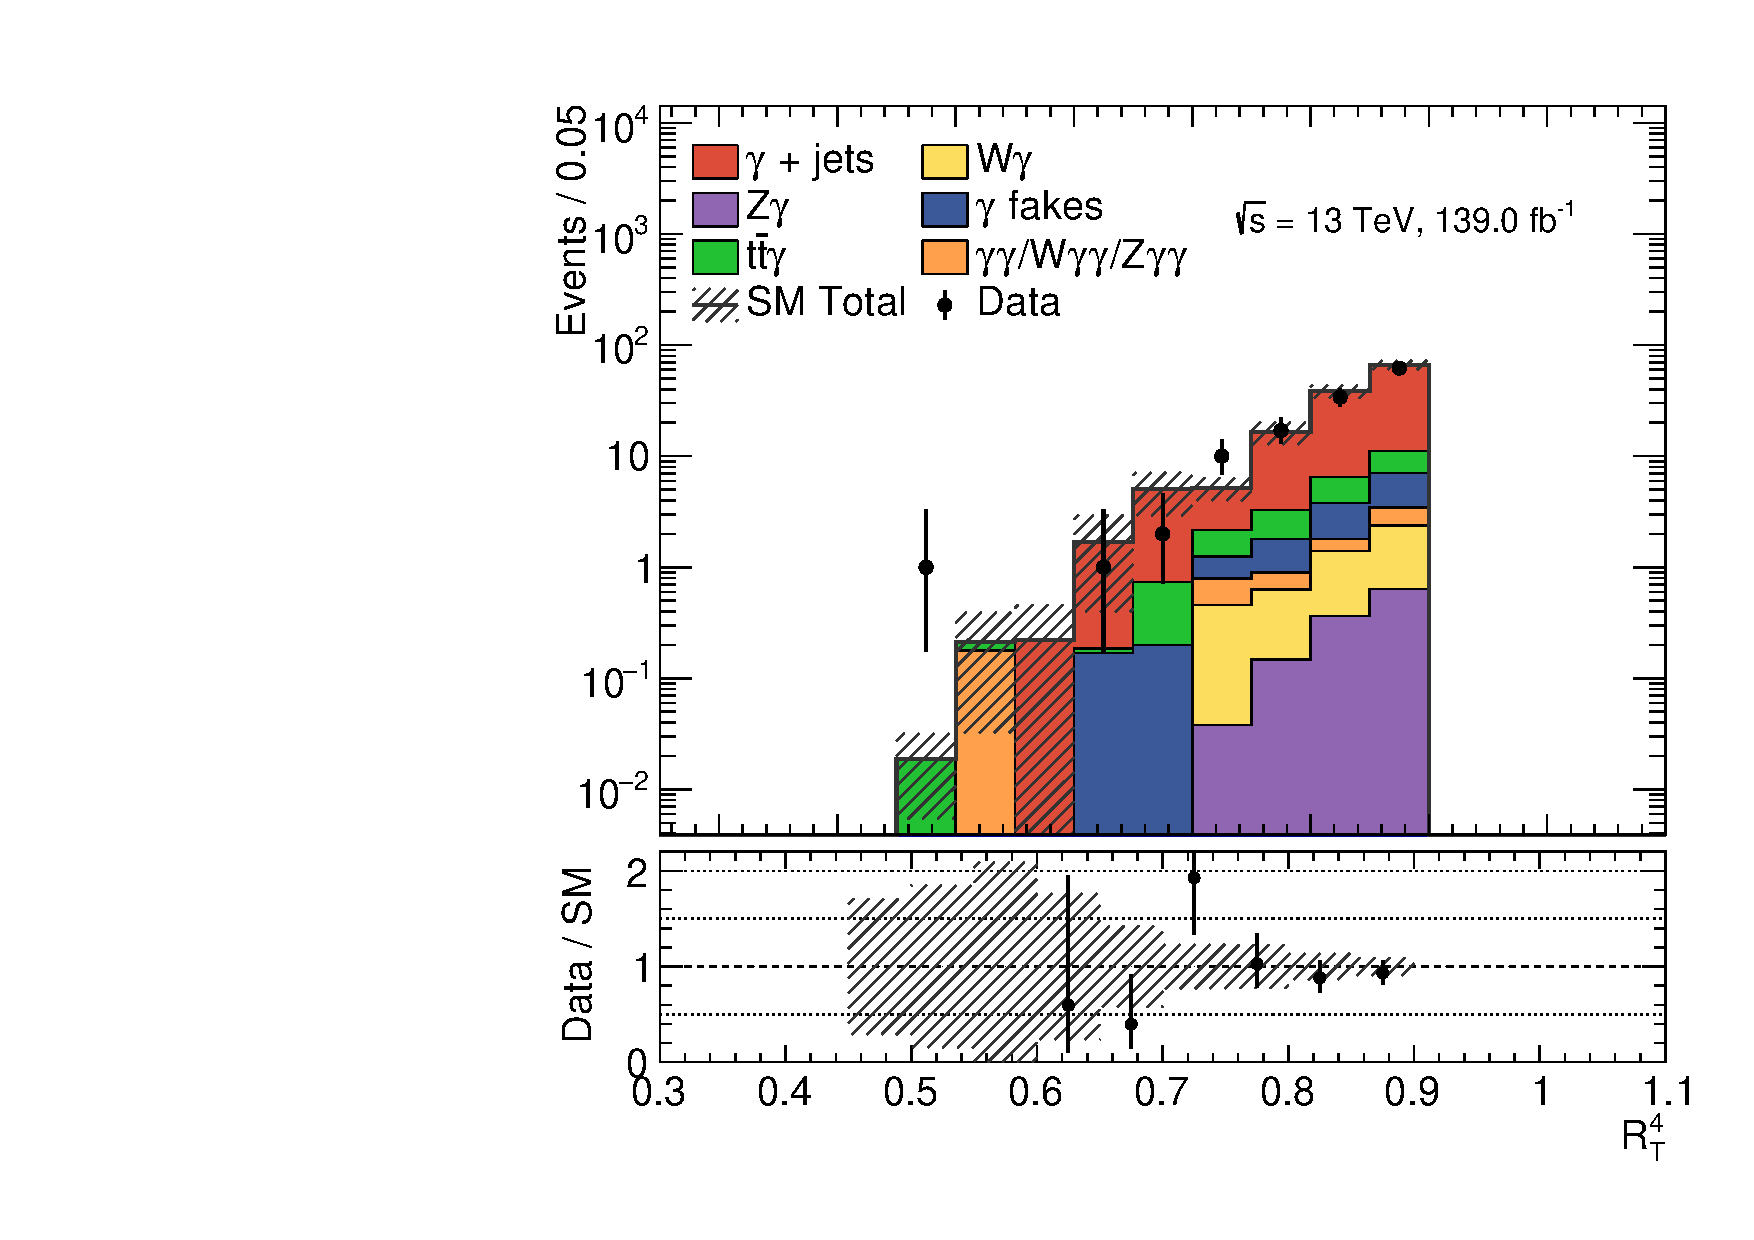
\includegraphics[width=0.32\textwidth]{images/results/fr2_unblind/can_VRM1L_rt4_afterFit.pdf}
    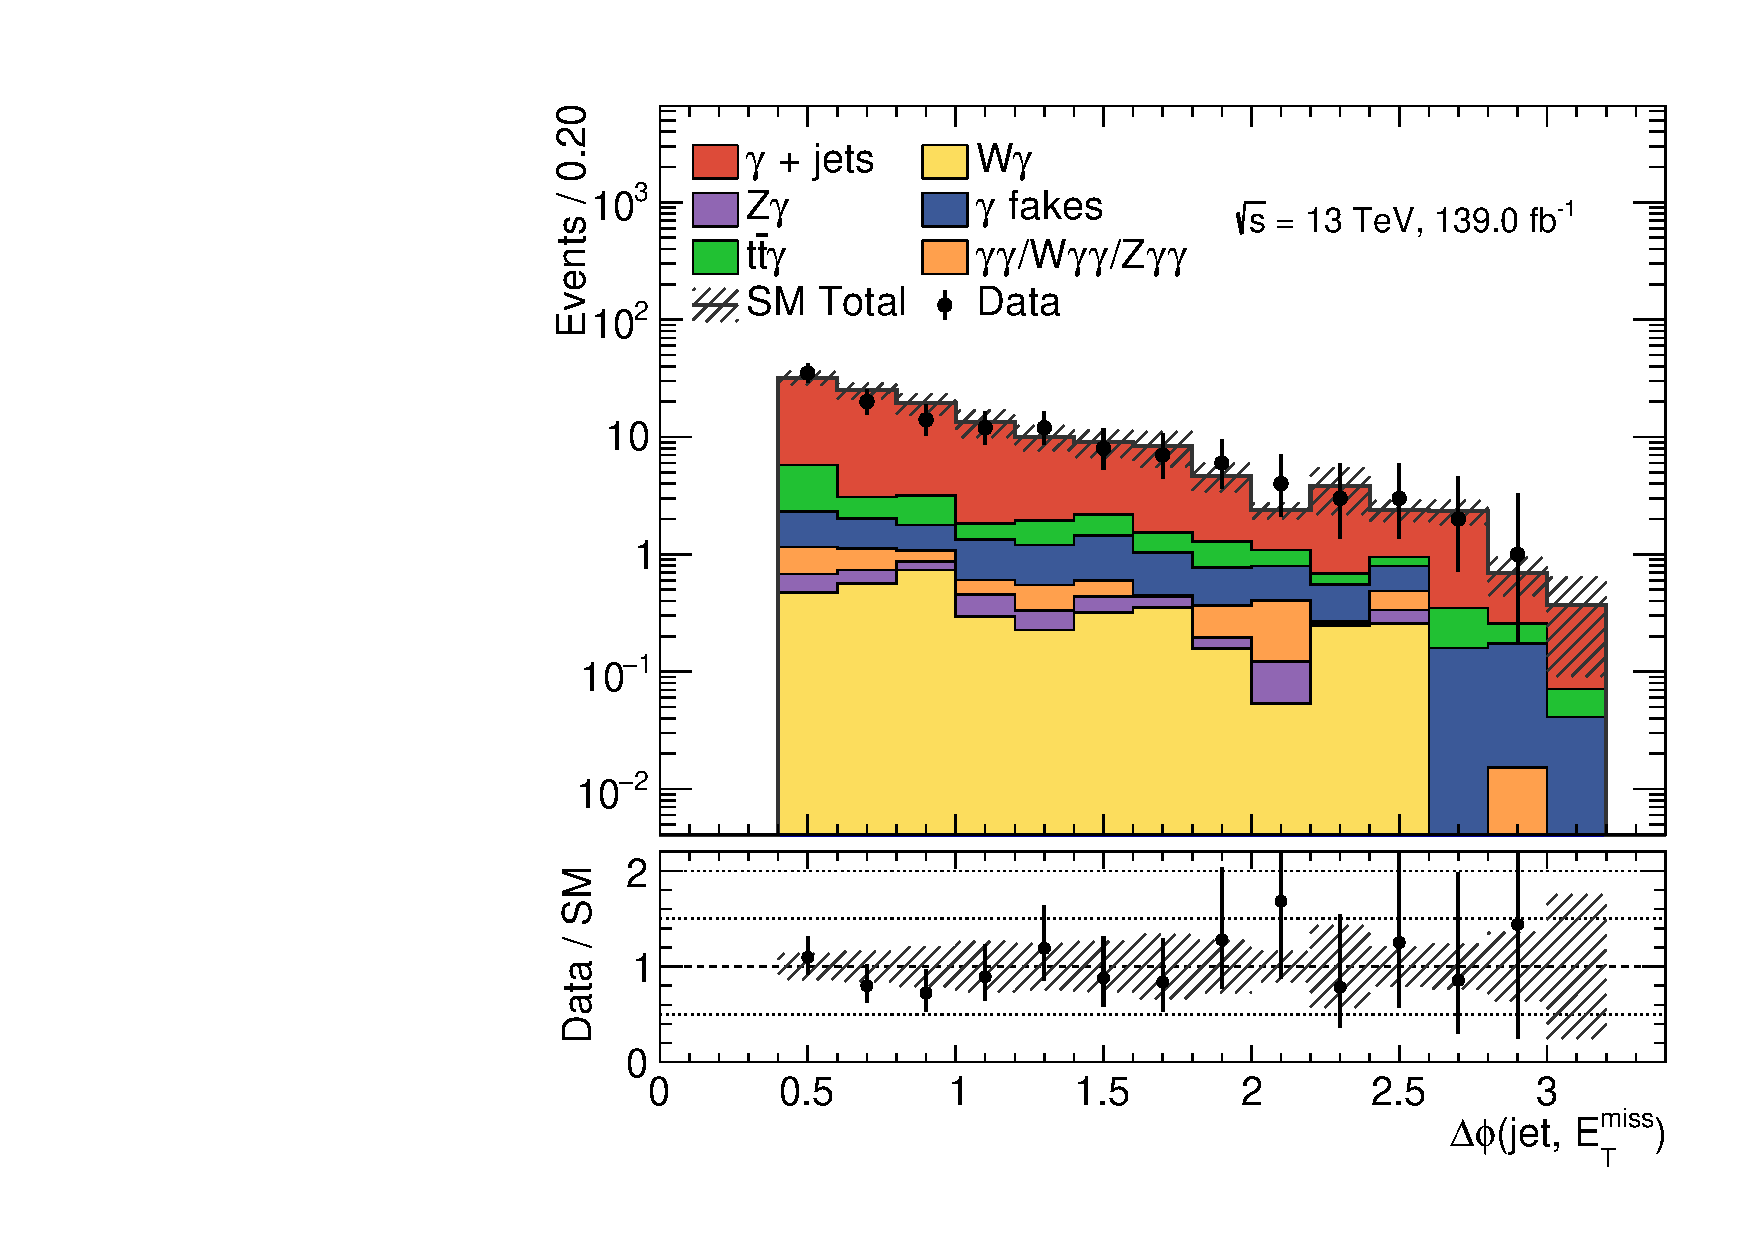
\includegraphics[width=0.32\textwidth]{images/results/fr2_unblind/can_VRM1L_dphi_jetmet_afterFit.pdf}

    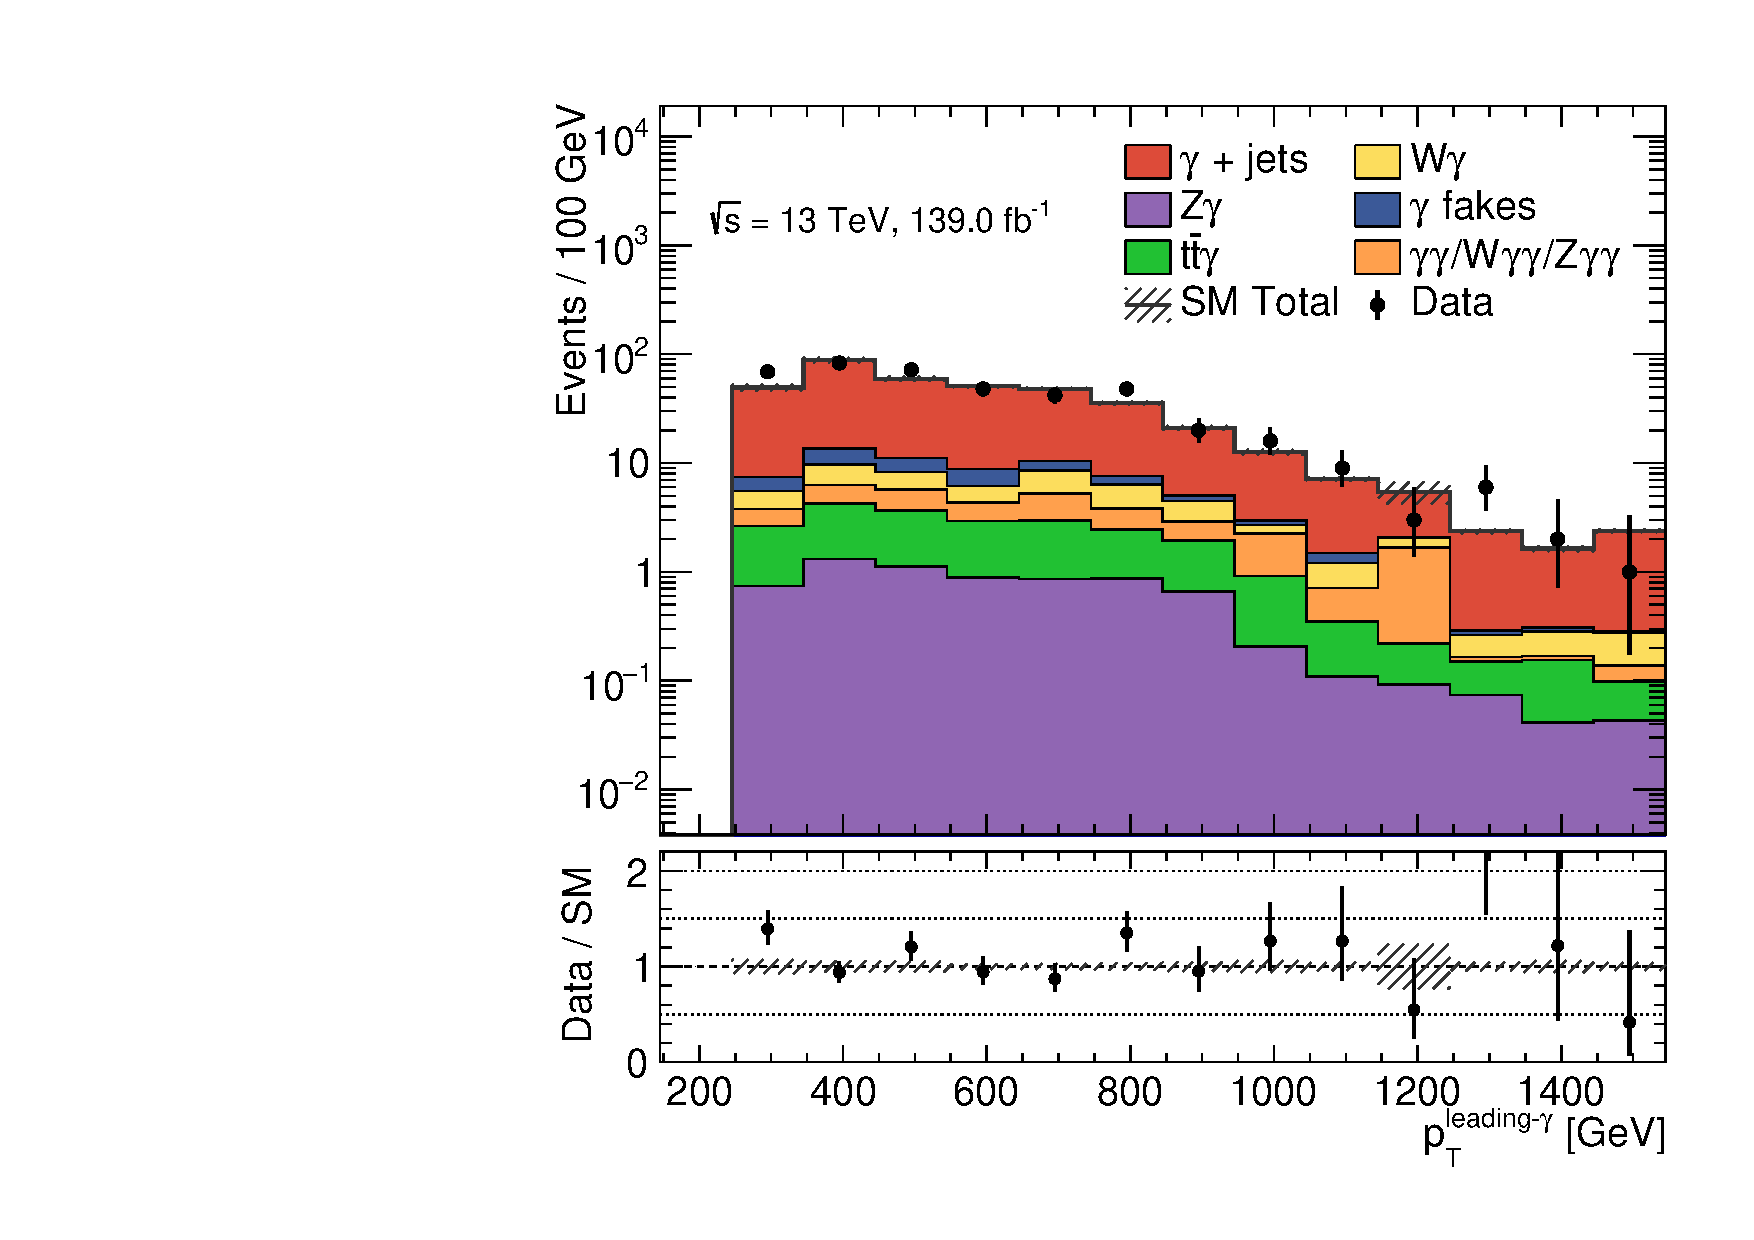
\includegraphics[width=0.32\textwidth]{images/results/fr2_unblind/can_VRM1H_ph_pt0_afterFit.pdf}
    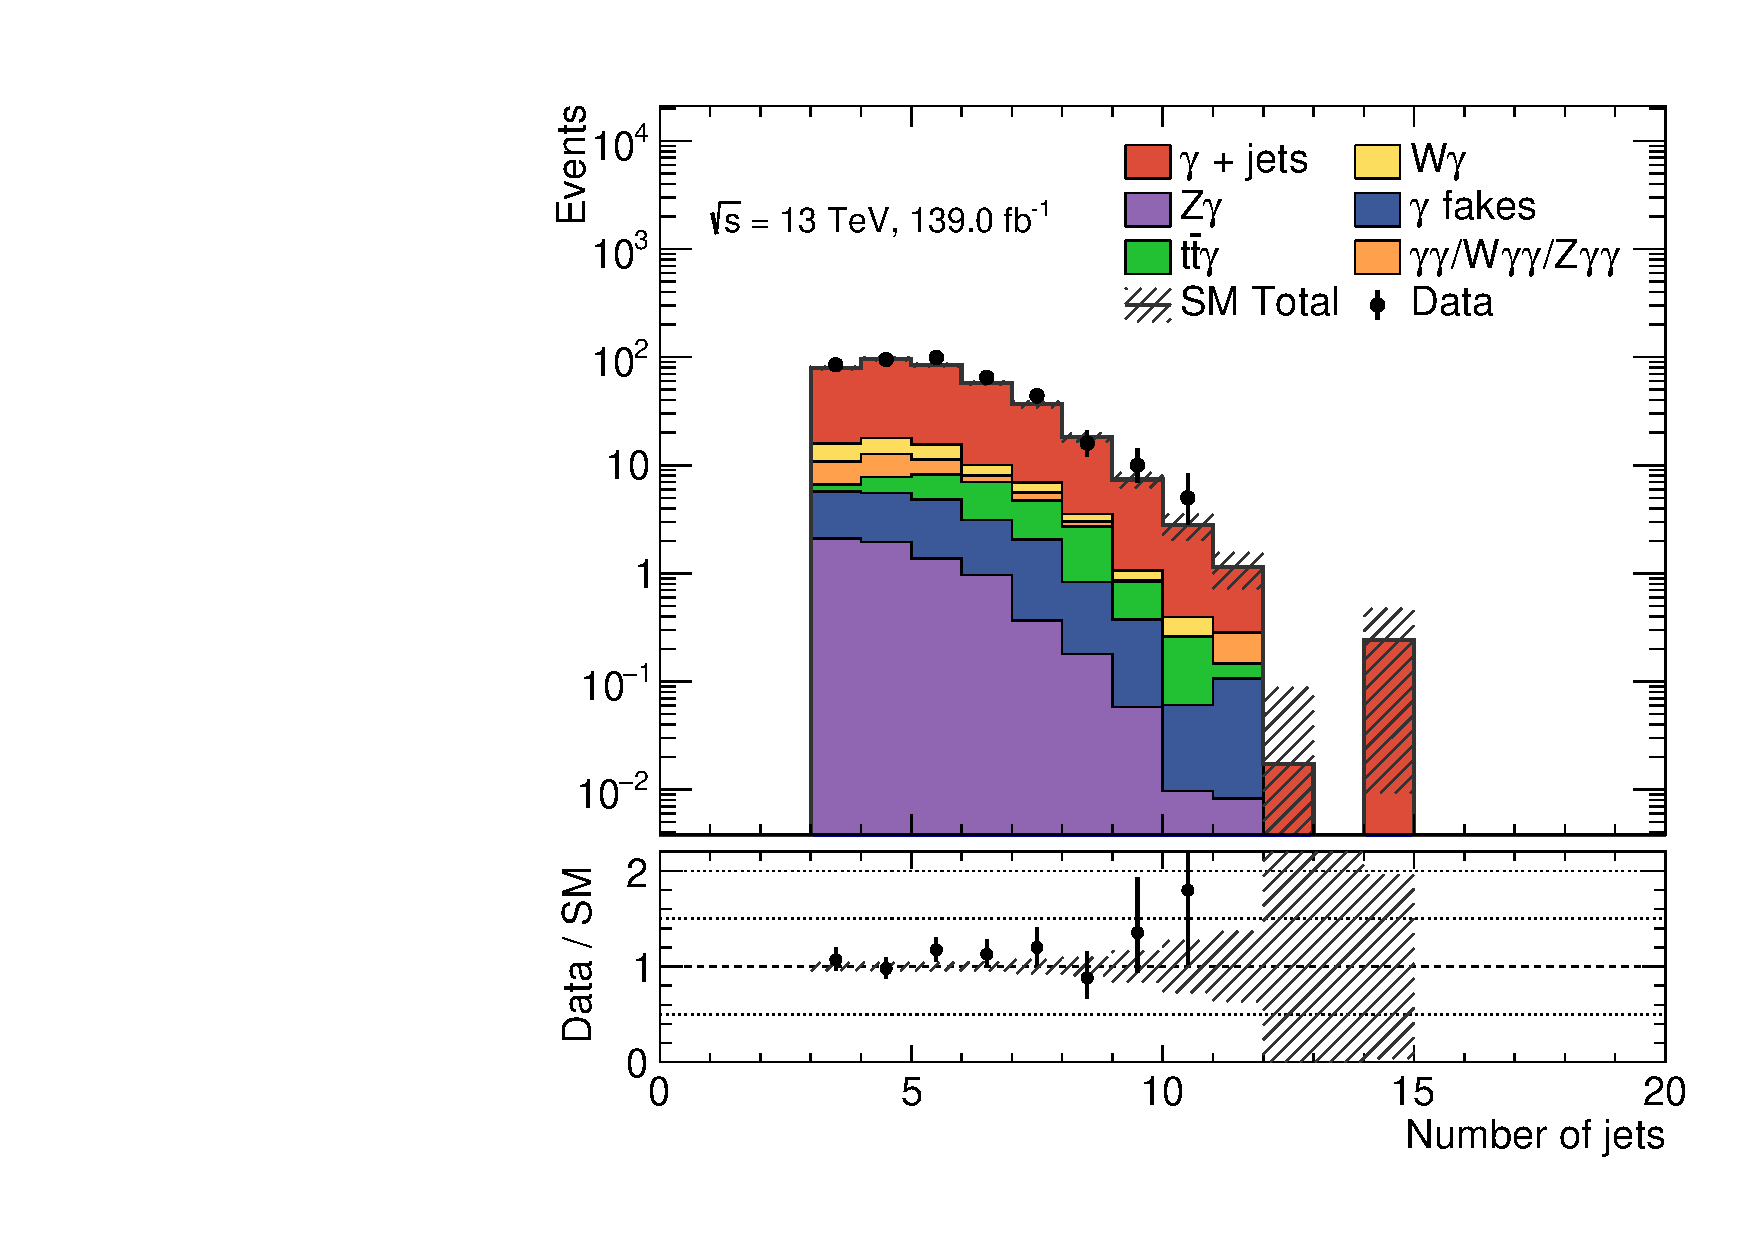
\includegraphics[width=0.32\textwidth]{images/results/fr2_unblind/can_VRM1H_jet_n_afterFit.pdf}
    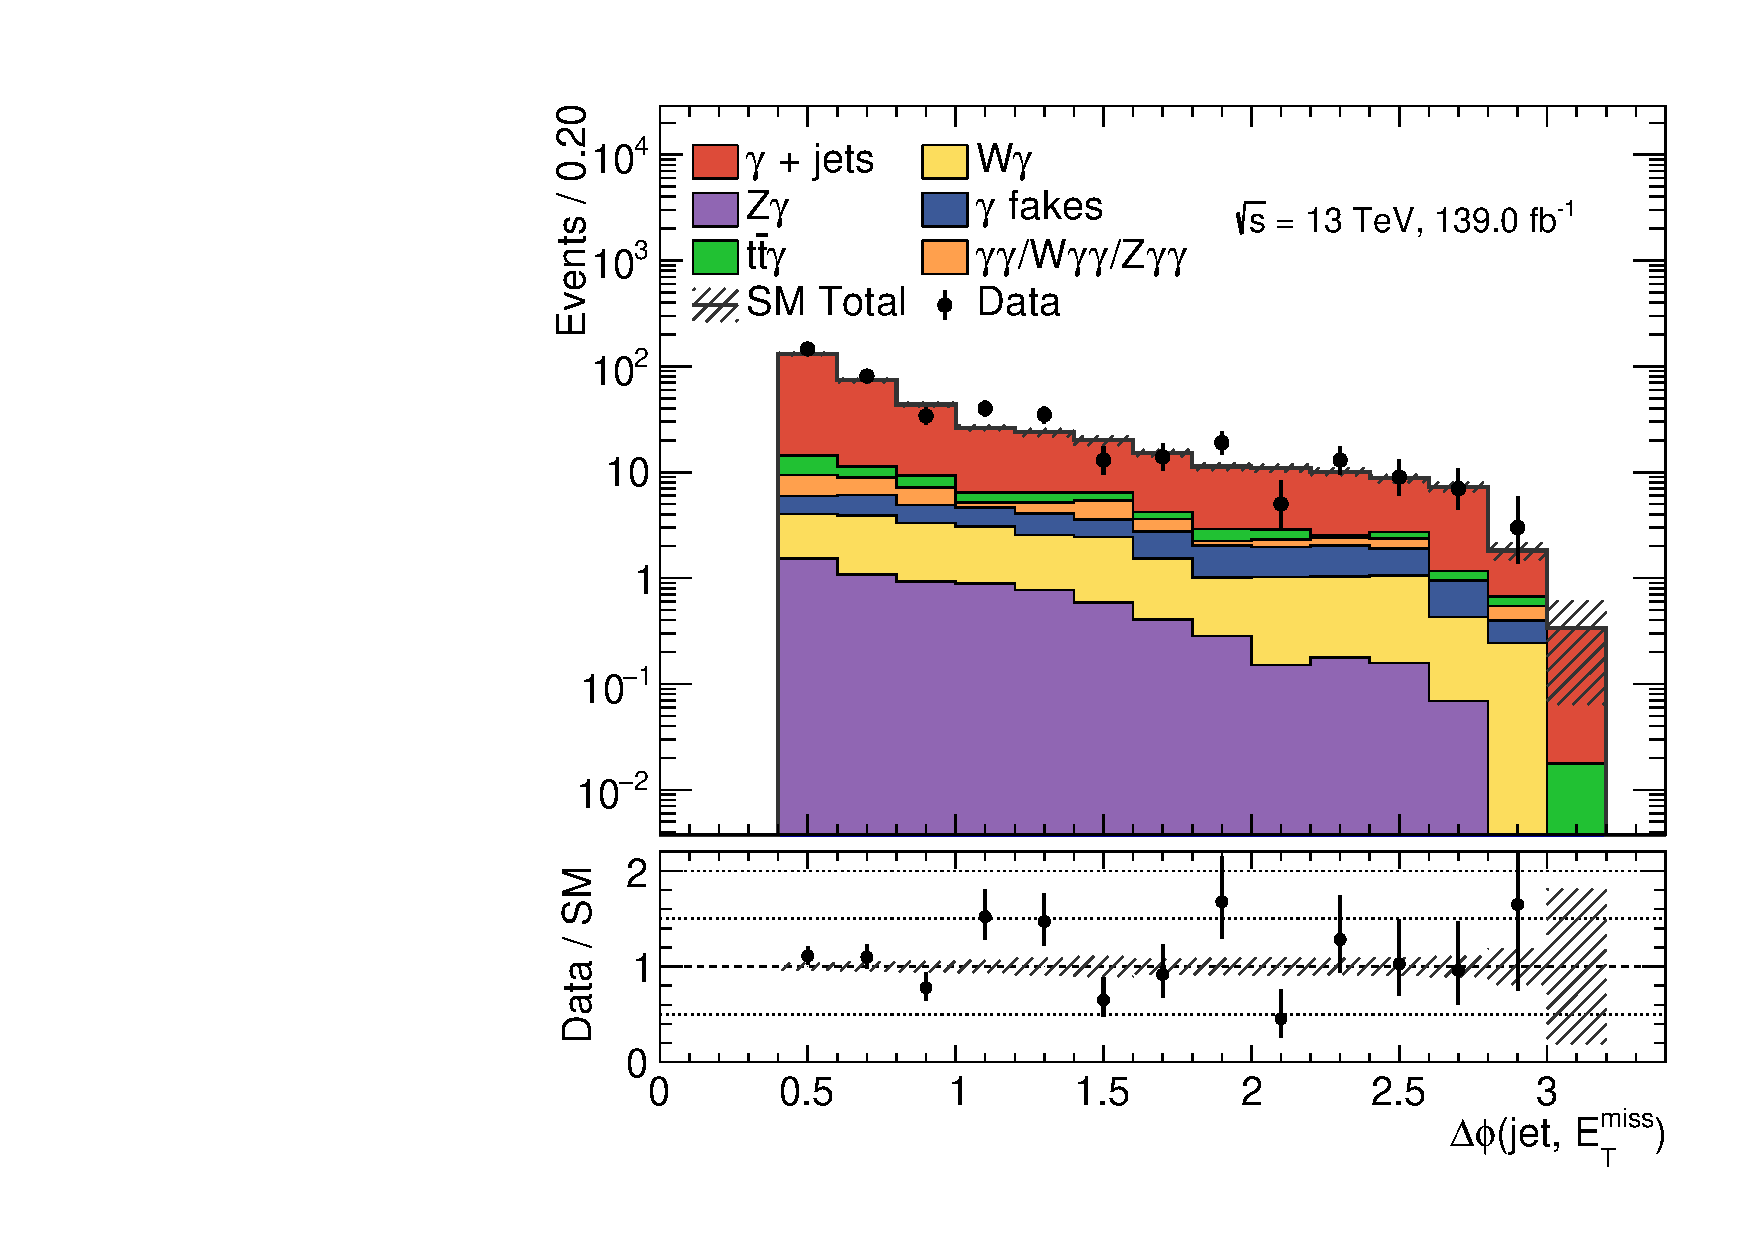
\includegraphics[width=0.32\textwidth]{images/results/fr2_unblind/can_VRM1H_dphi_jetmet_afterFit.pdf}

    
    \caption{Distribuciones de algunas variables significativas en las regiones de validación VRQ (arriba), VRM1H (medio) y VRM1L (abajo) luego del ajuste de solo fondo. Las incertezas mostradas son sólo estadísticas.}
    \label{fig:dist_vrqm_bkgonly}
\end{figure}

\begin{figure}[ht!]
  \centering

    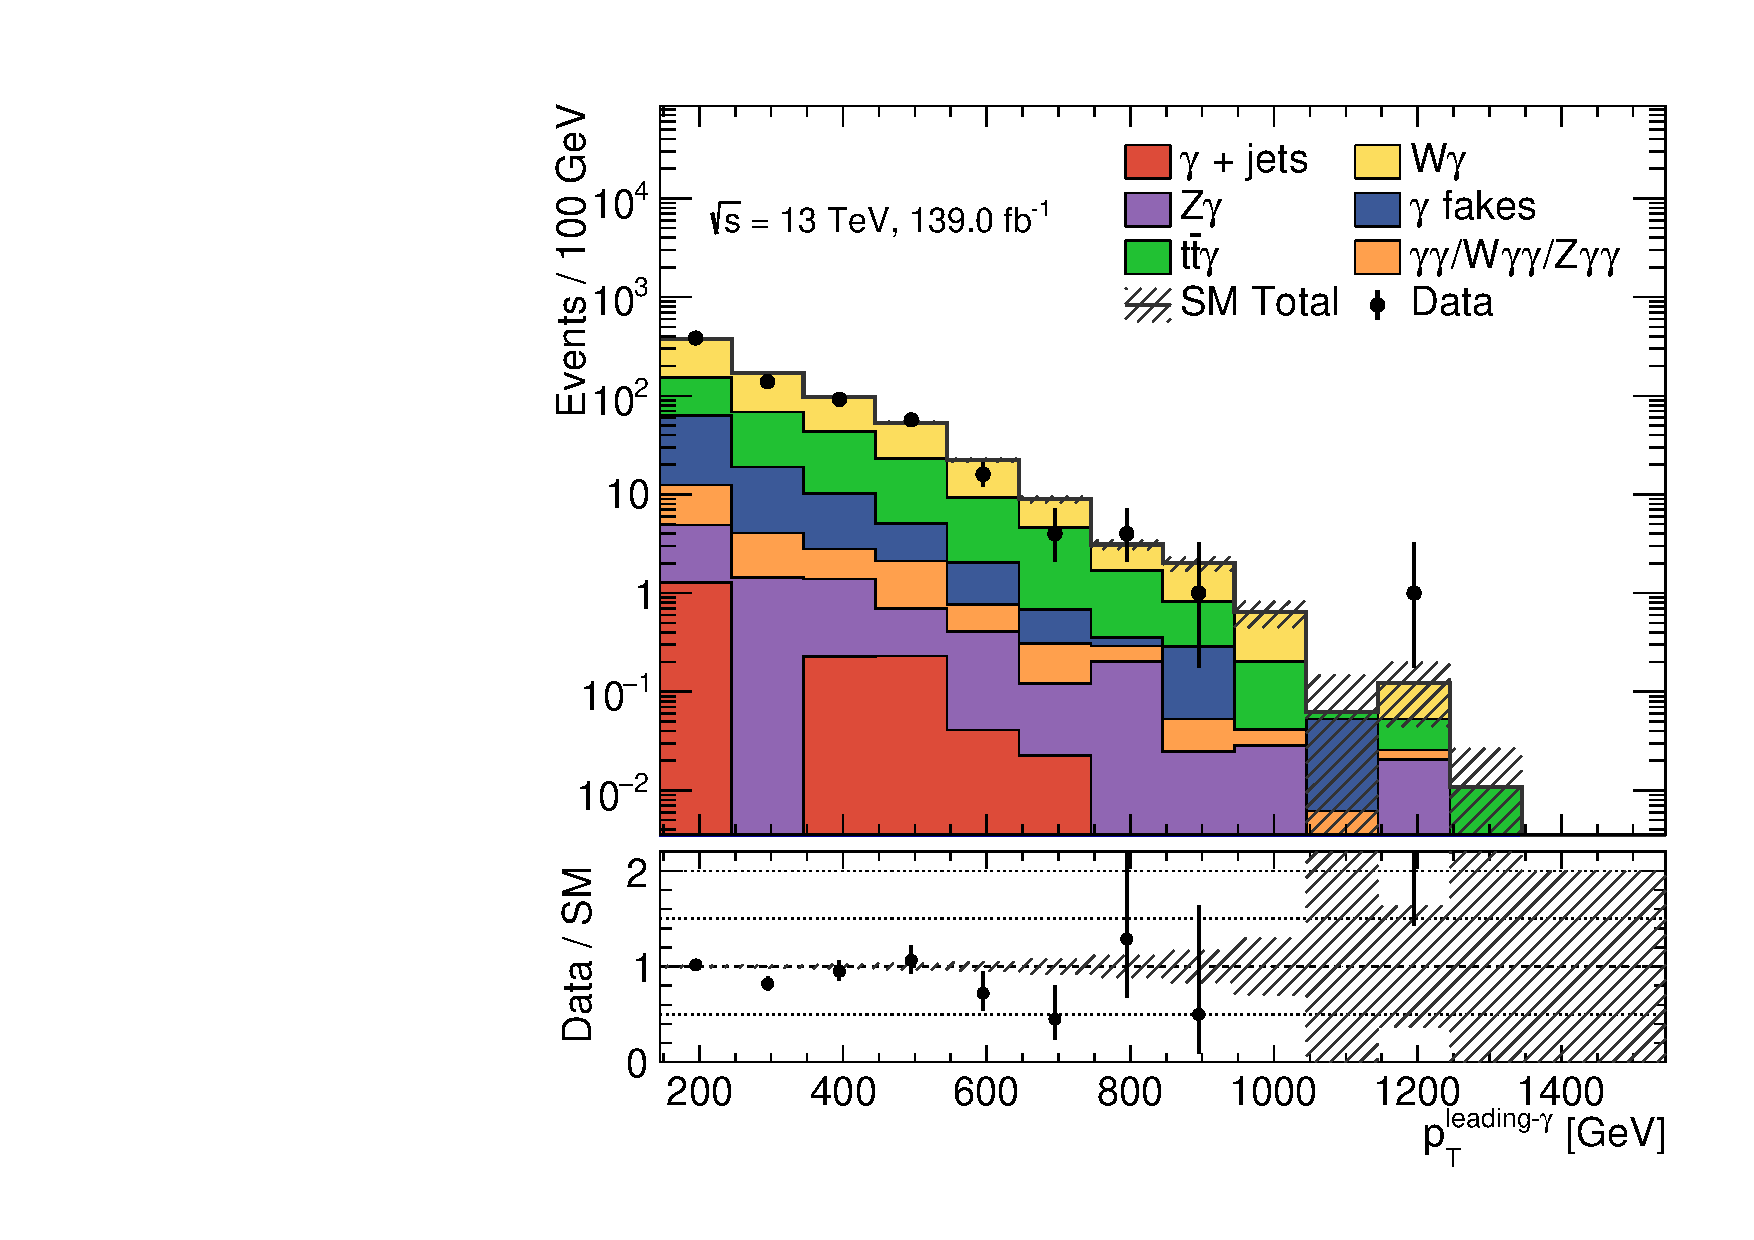
\includegraphics[width=0.32\textwidth]{images/results/fr2_unblind/can_VRL3_ph_pt0_afterFit.pdf}
    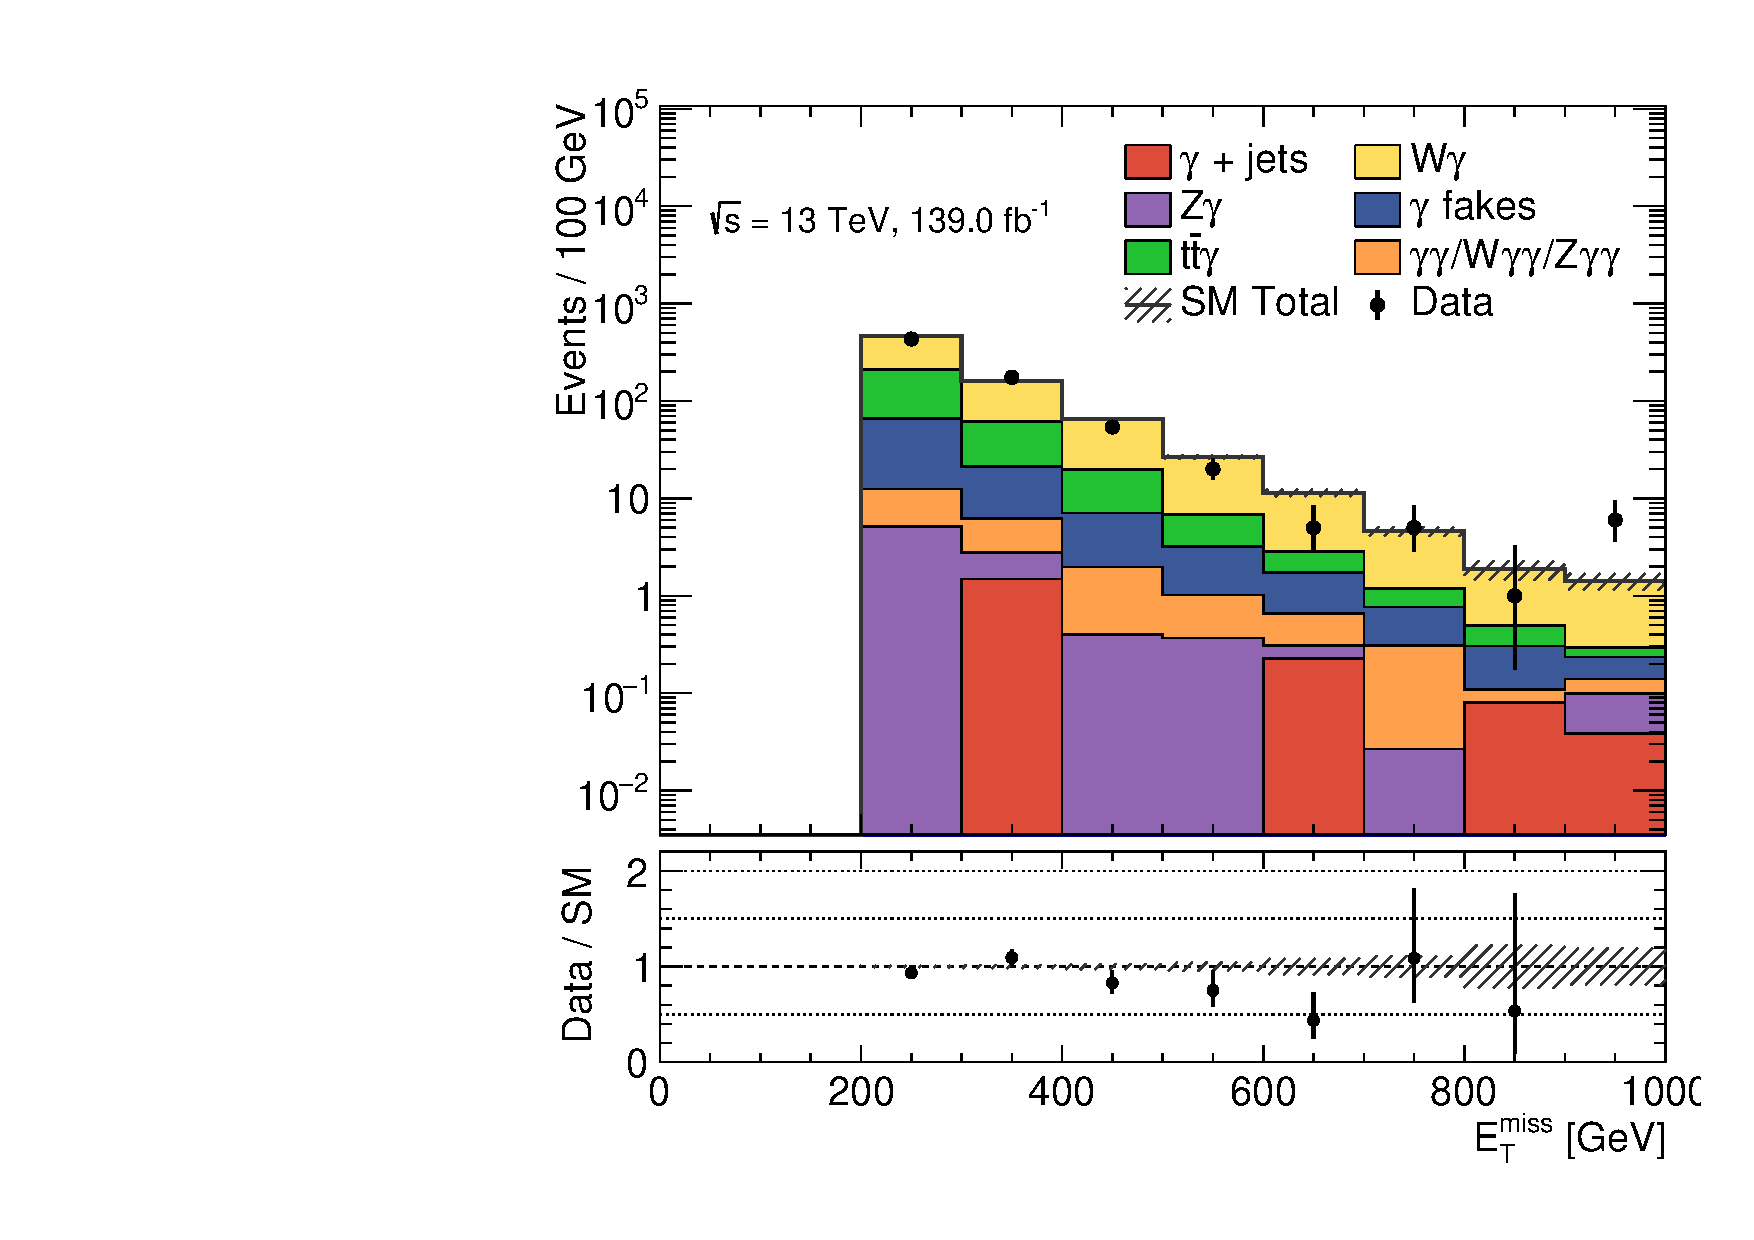
\includegraphics[width=0.32\textwidth]{images/results/fr2_unblind/can_VRL3_met_et_afterFit.pdf}
    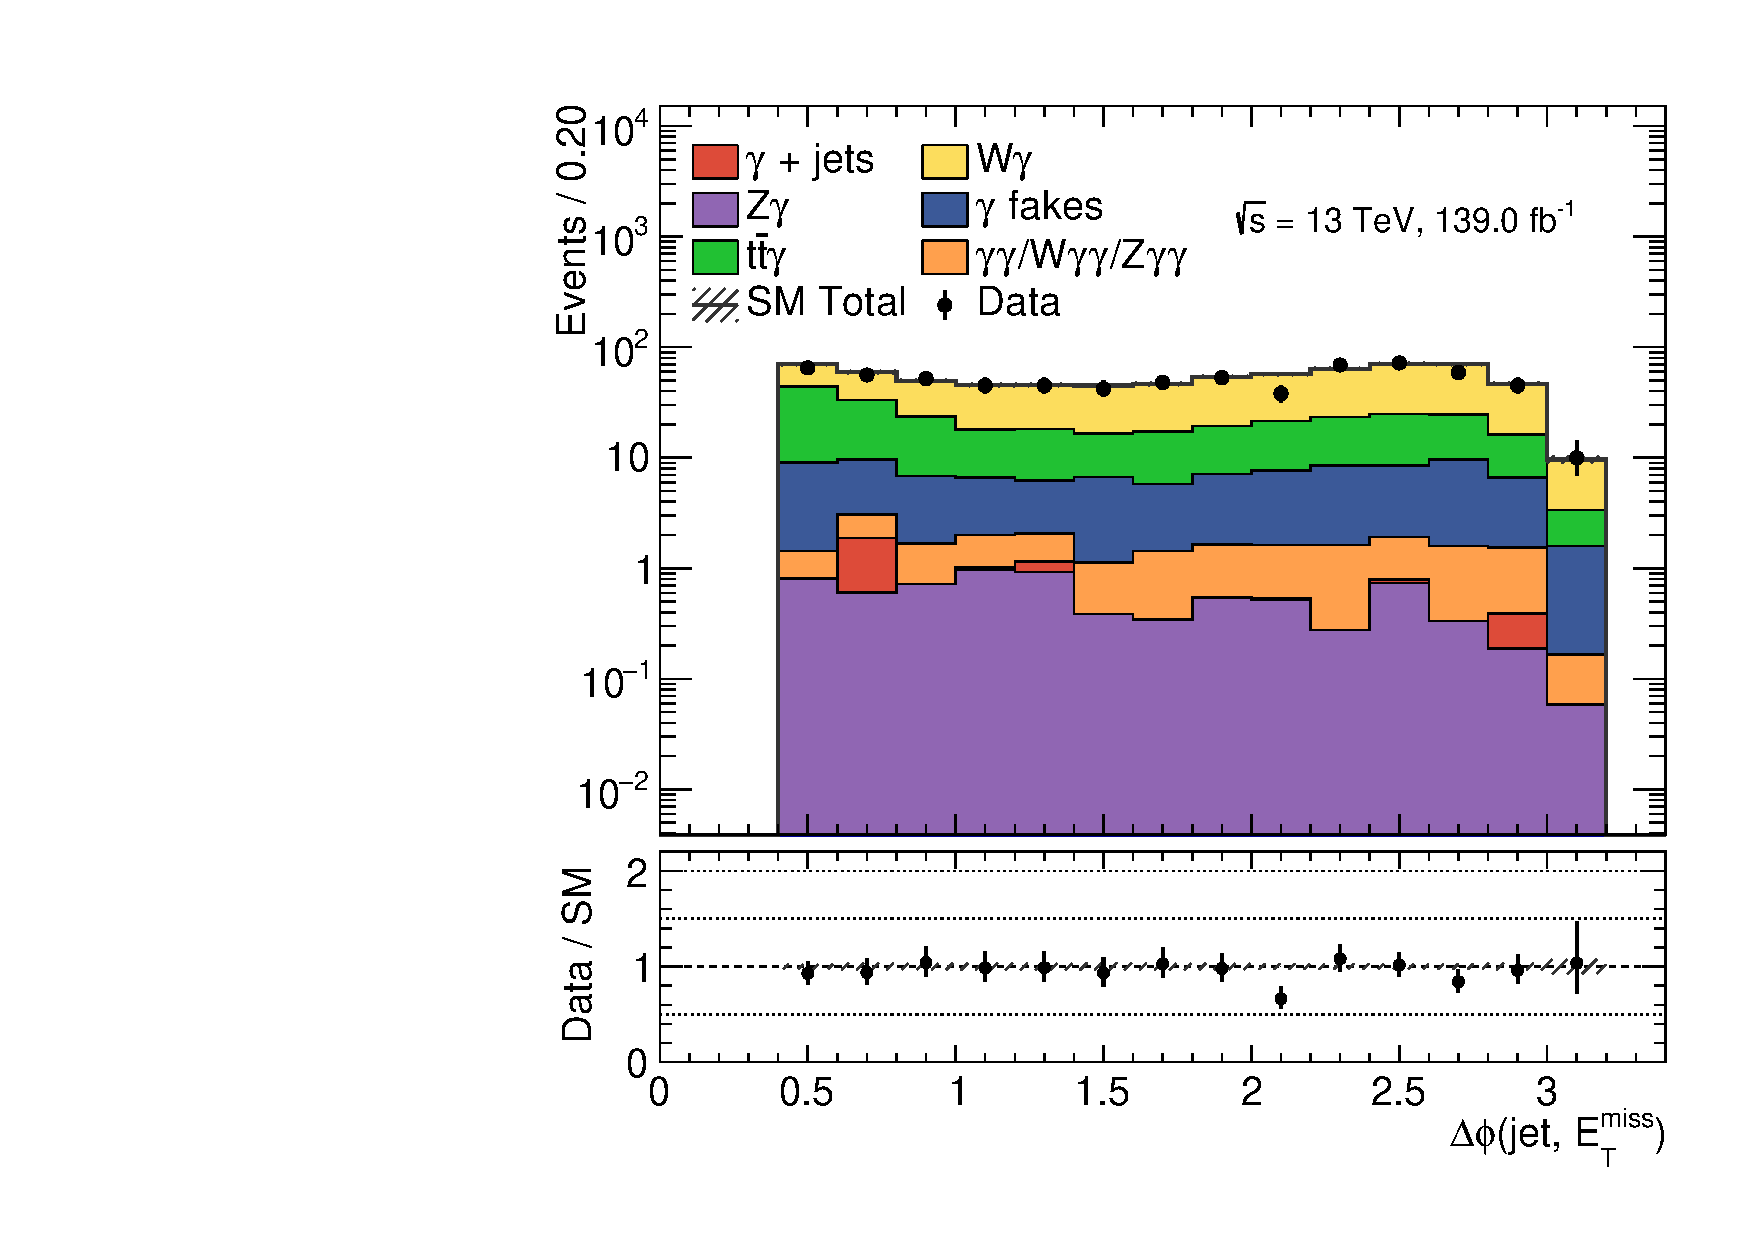
\includegraphics[width=0.32\textwidth]{images/results/fr2_unblind/can_VRL3_dphi_jetmet_afterFit.pdf}

    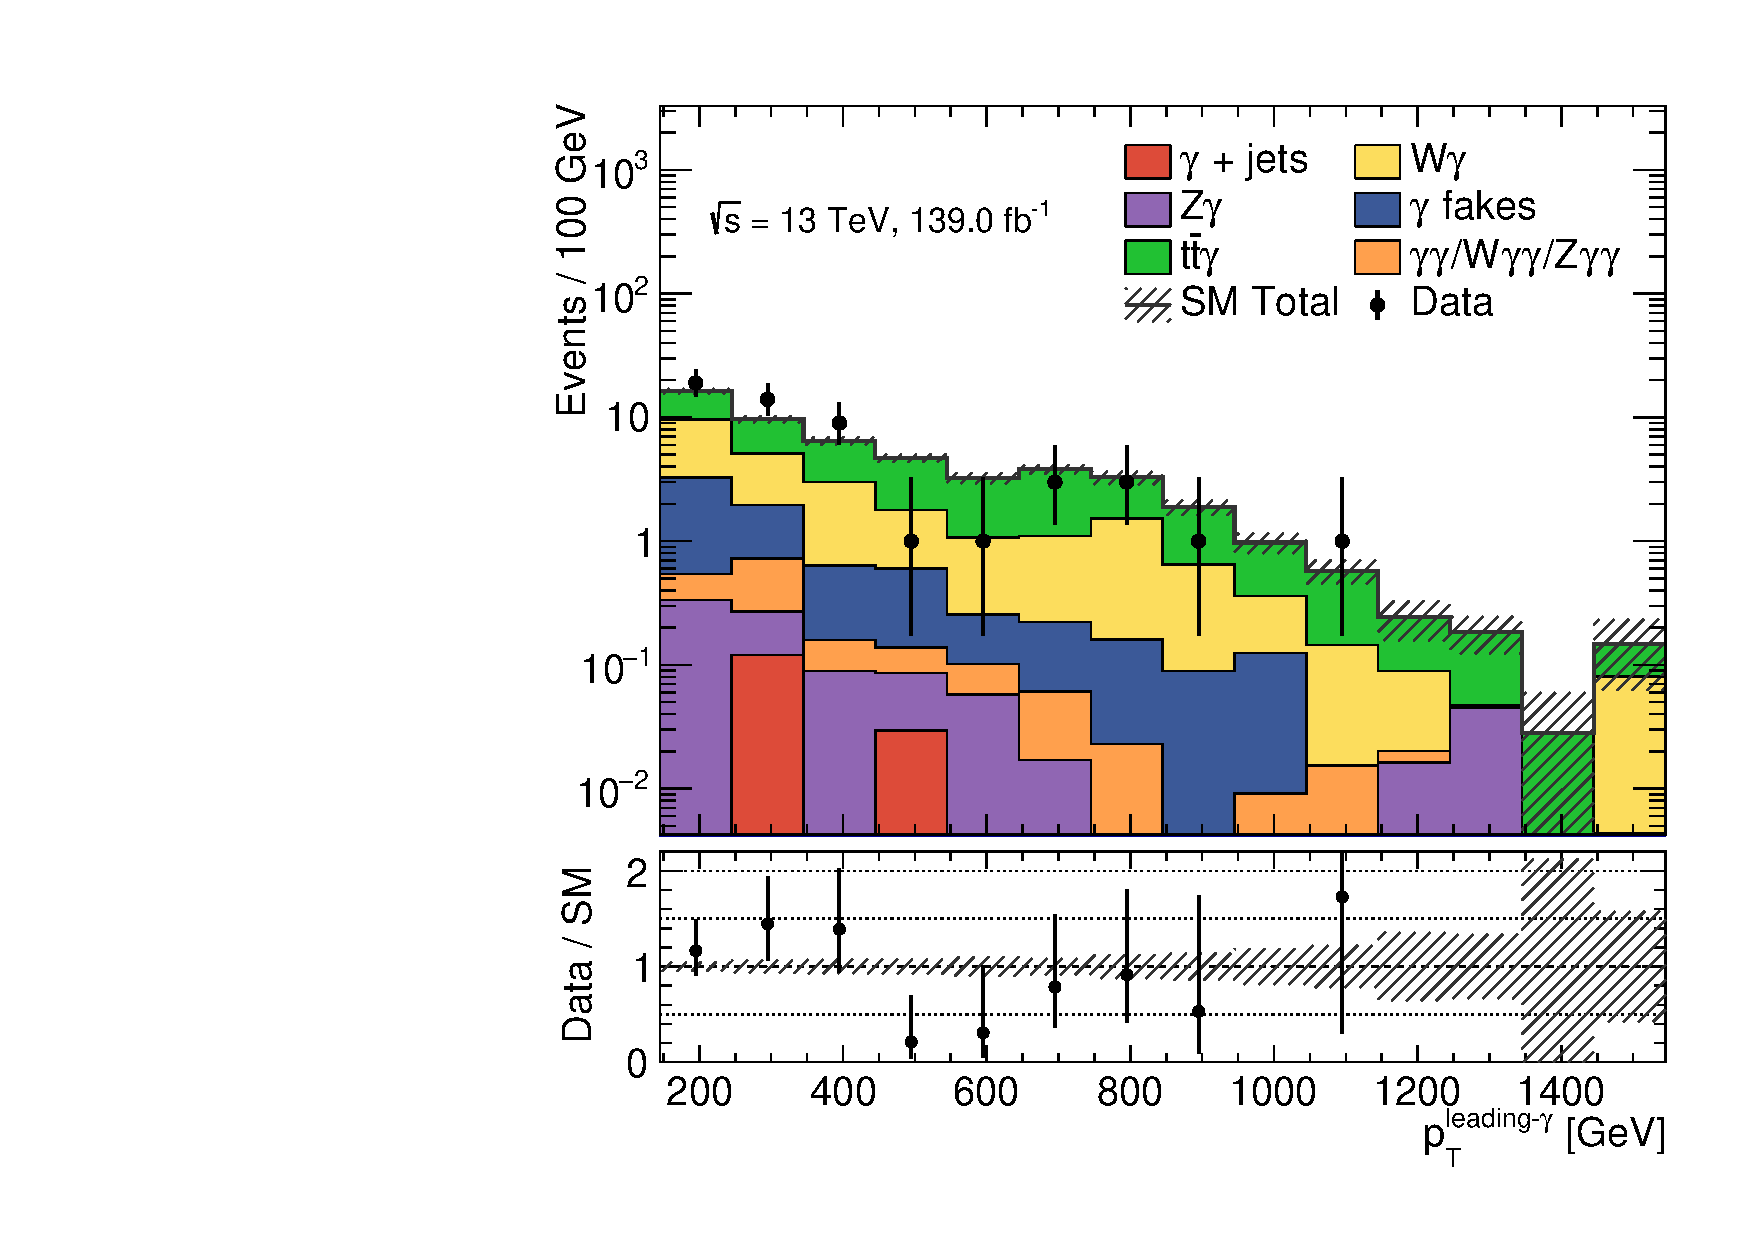
\includegraphics[width=0.32\textwidth]{images/results/fr2_unblind/can_VRL4_ph_pt0_afterFit.pdf}
    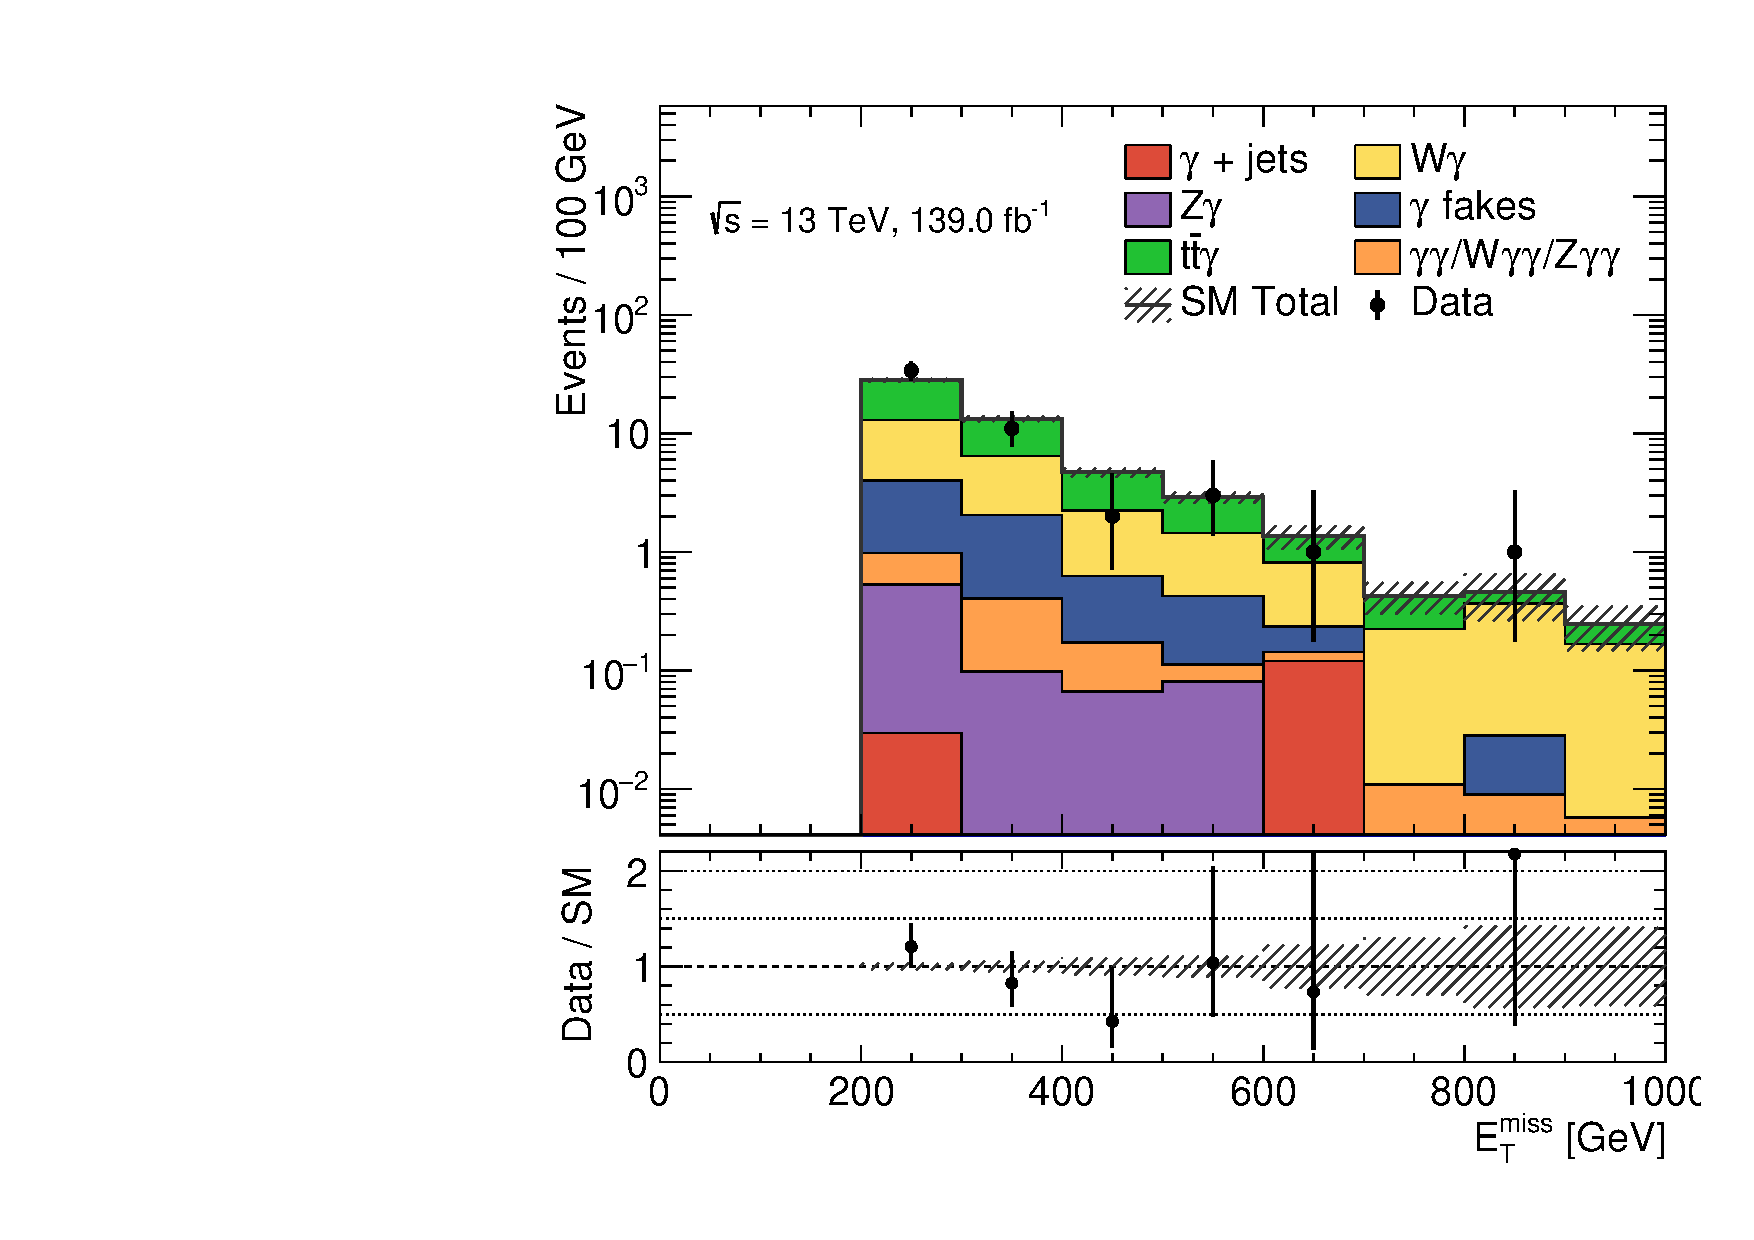
\includegraphics[width=0.32\textwidth]{images/results/fr2_unblind/can_VRL4_met_et_afterFit.pdf}
    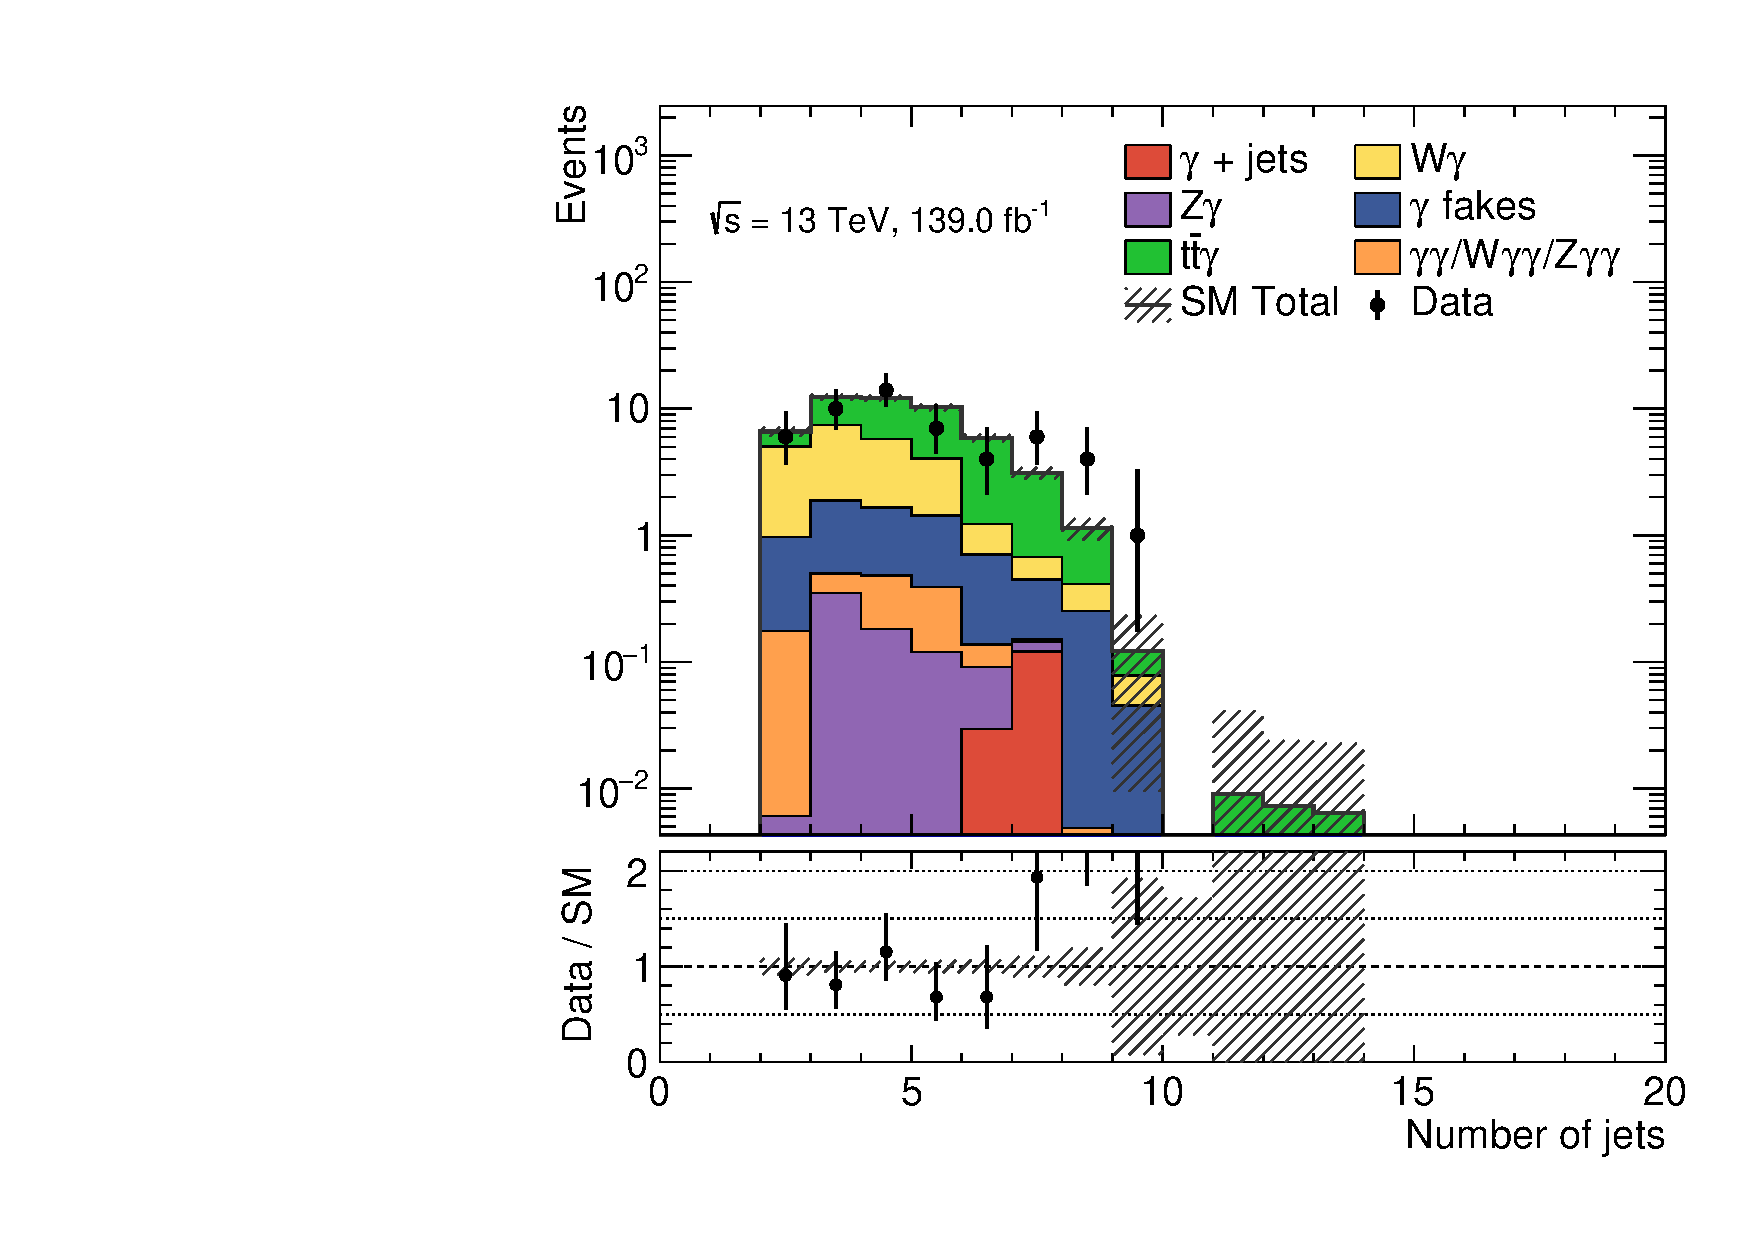
\includegraphics[width=0.32\textwidth]{images/results/fr2_unblind/can_VRL4_jet_n_afterFit.pdf}

    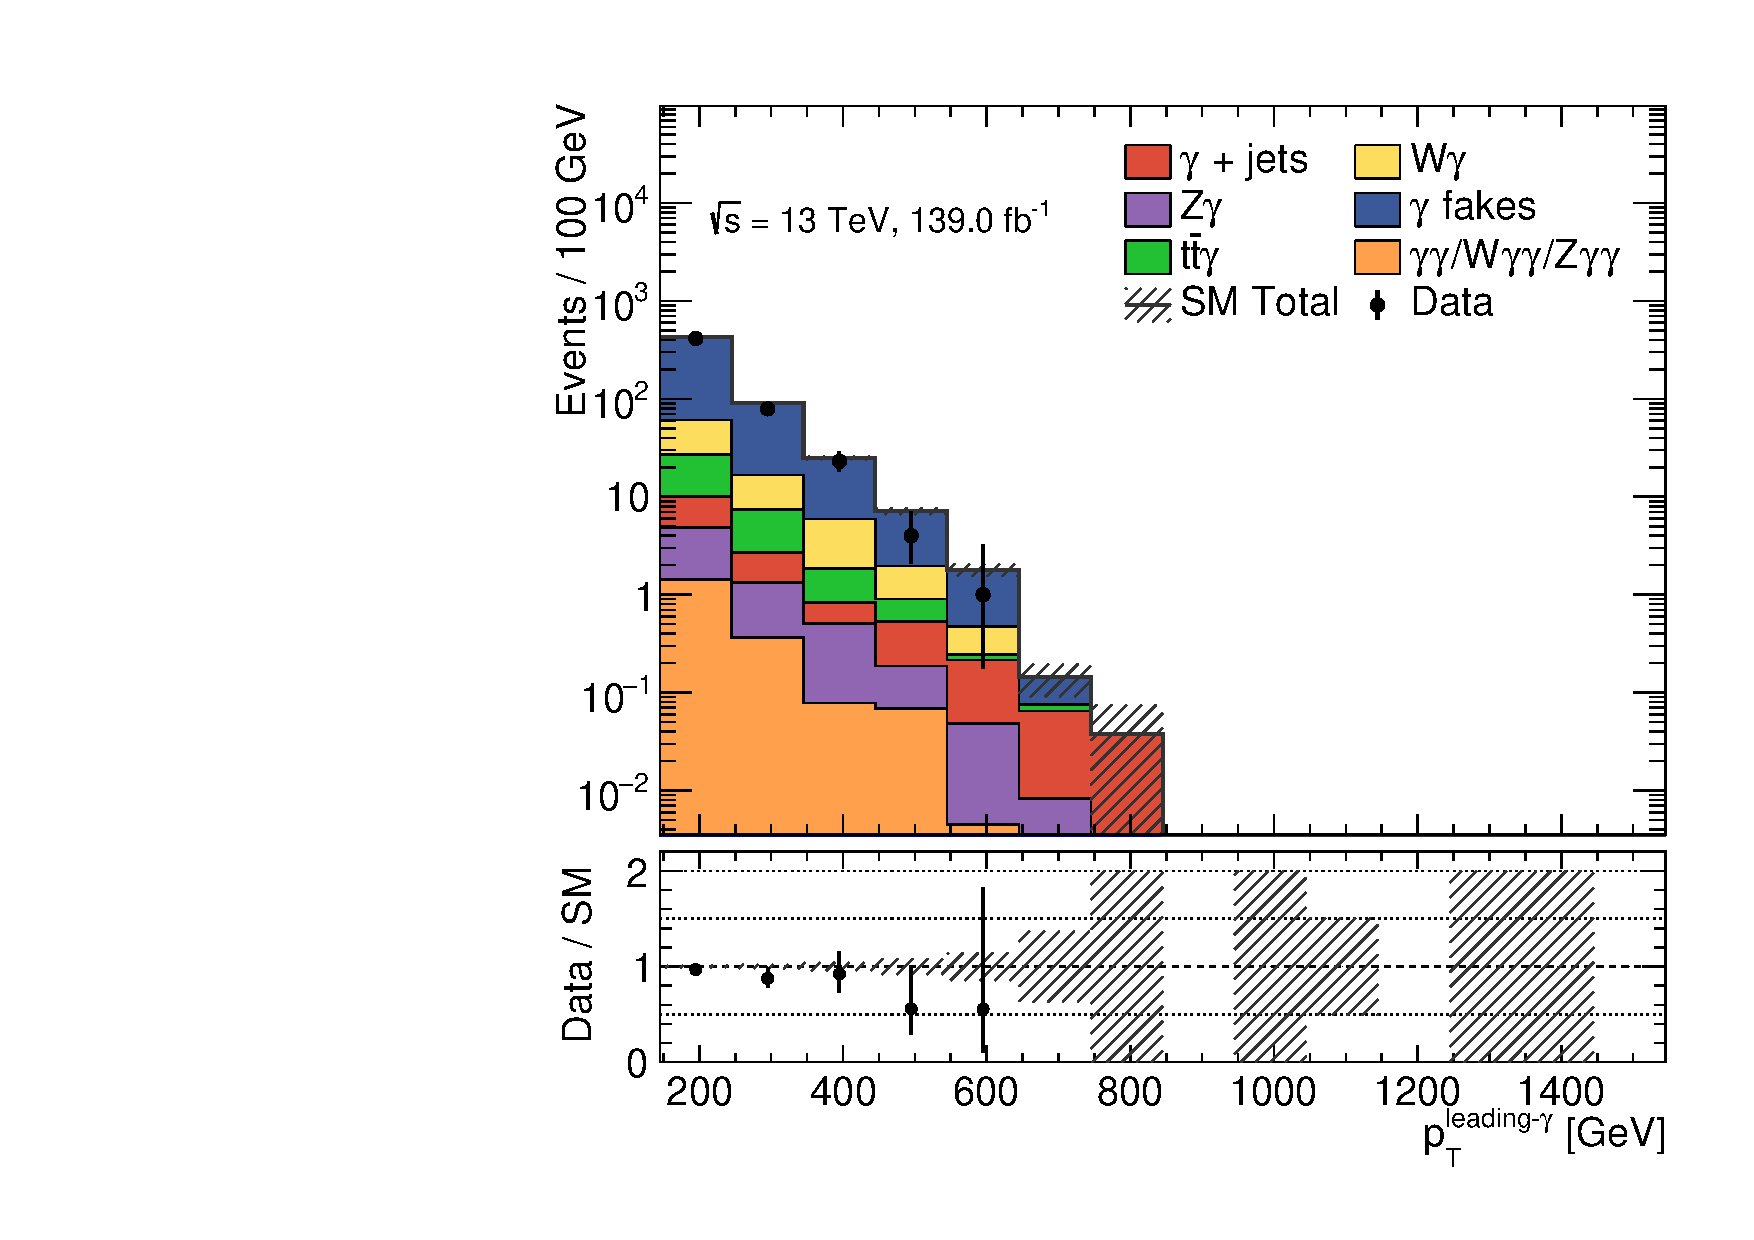
\includegraphics[width=0.32\textwidth]{images/results/fr2_unblind/can_VRE_ph_pt0_afterFit.pdf}
    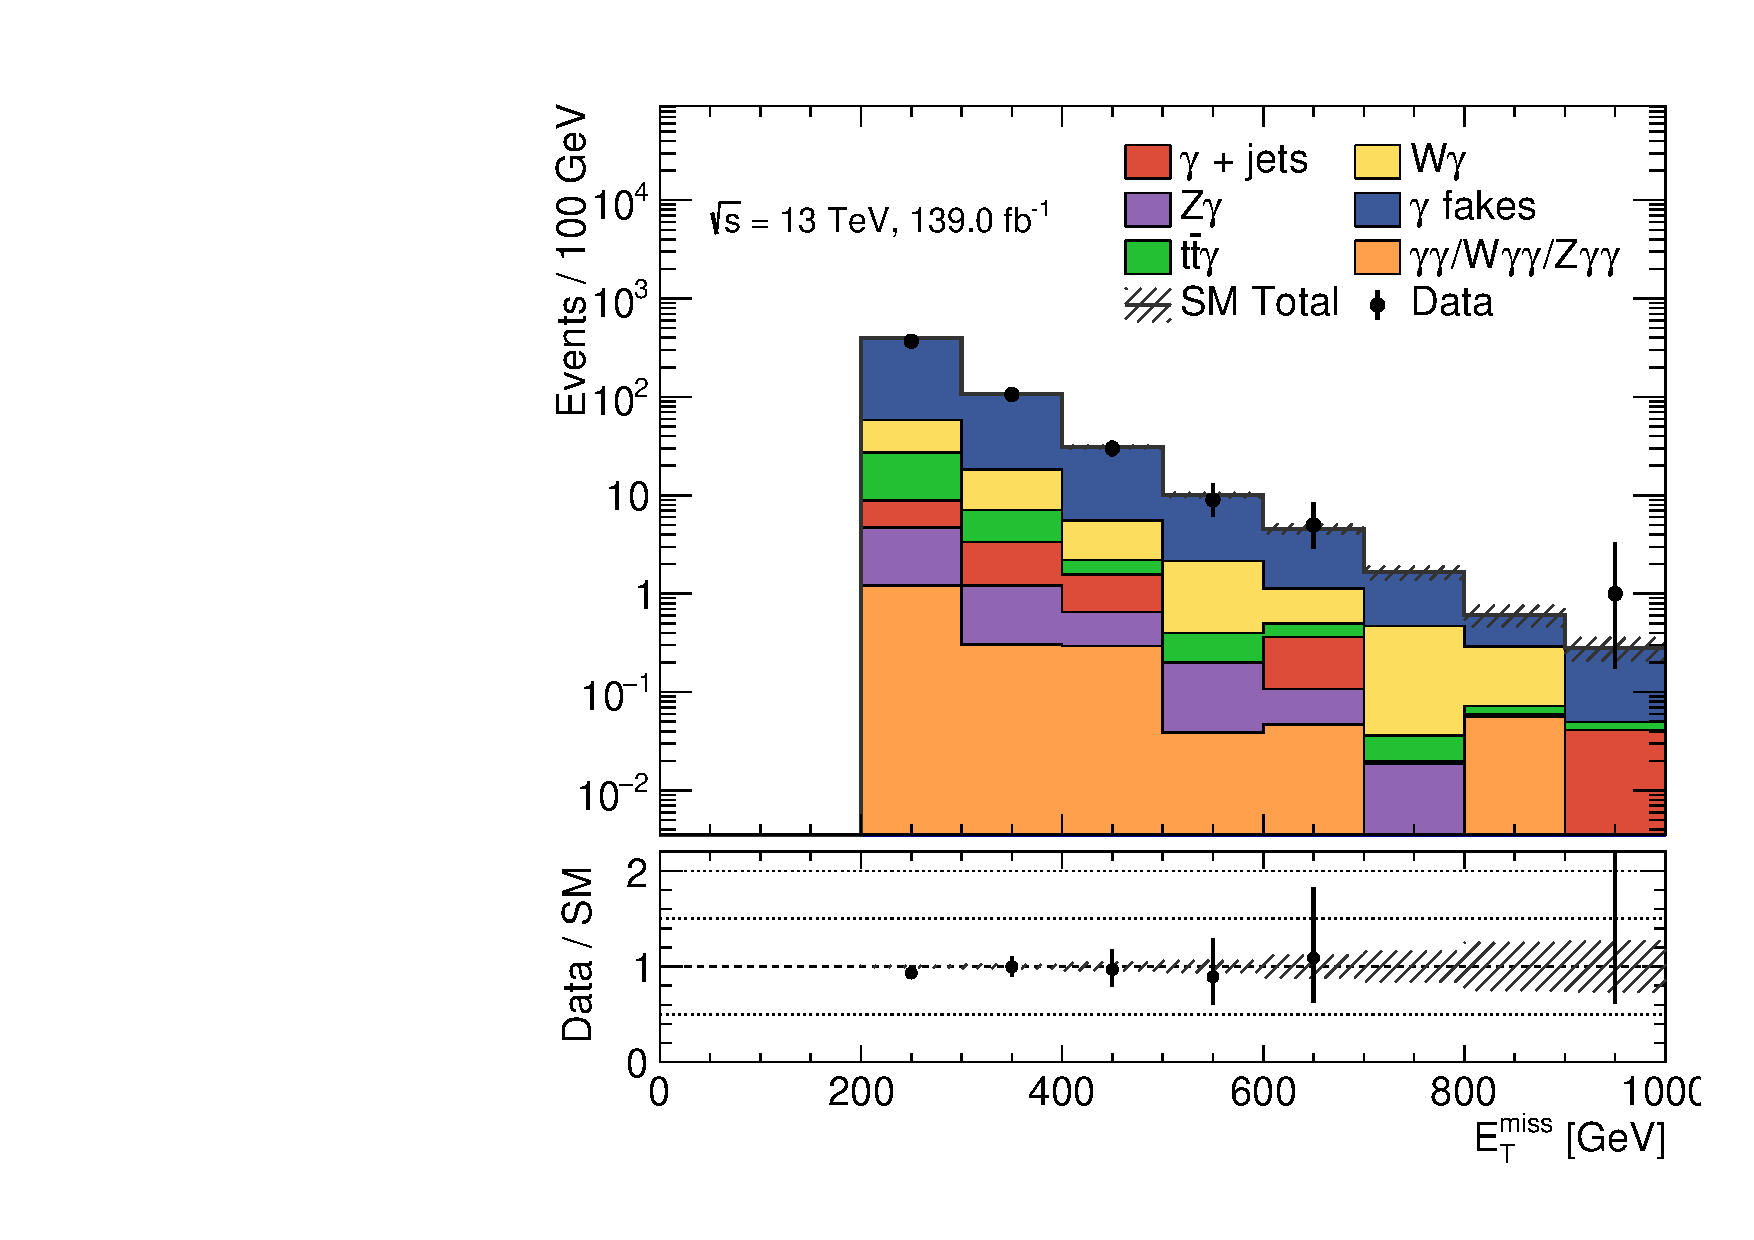
\includegraphics[width=0.32\textwidth]{images/results/fr2_unblind/can_VRE_met_et_afterFit.pdf}
    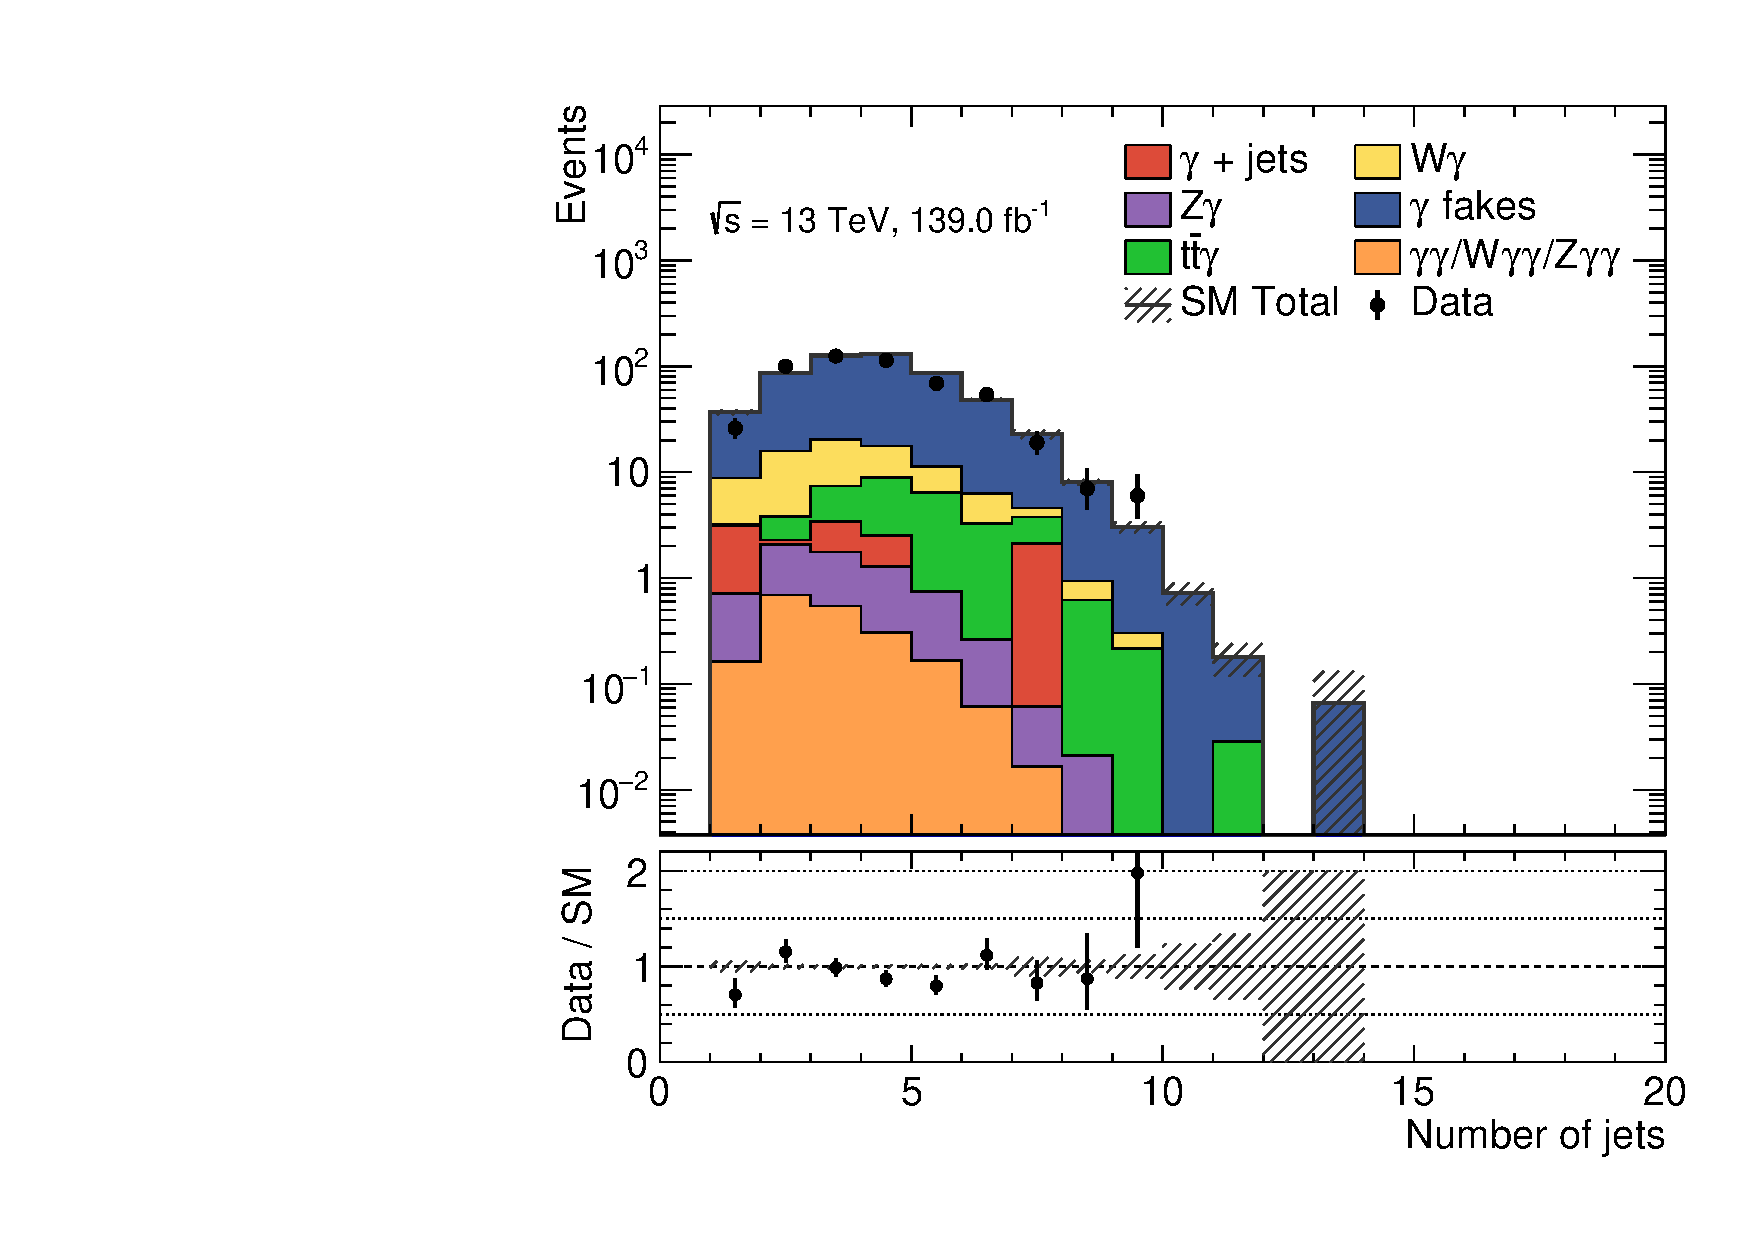
\includegraphics[width=0.32\textwidth]{images/results/fr2_unblind/can_VRE_jet_n_afterFit.pdf}

    
    \caption{Distribuciones de algunas variables significativas en las regiones de validación VRL3 (arriba), VRL4 (medio) y VRE (abajo) luego del ajuste de solo fondo. Las incertezas mostradas son sólo estadísticas.}
    \label{fig:dist_vrle_bkgonly}
\end{figure}


% \solved{Cosas que no estoy poniendo: signal contamination en las VRs, correlacion parametros del ajuste, tabla de incertezas sistematicas, pull de los NPs} solo tabla de sistematicos




\subsection{Resultados en las regiones de señal}

Luego de la estimación de los fondos en las regiones de señal y su correcta validación en sus respectivas VRs, se procedió a la observación de los datos en dichas regiones. En la Tabla \ref{tab:fit_result_sr_unblinded} se muestra el número de eventos observados y la estimación de los fondos en cada región de señal. El número total de eventos observados para la SRL es de $2$, para la SRM de $0$ y para la SRH de $5$, mientras que el número de eventos esperados es de $2.67\pm0.75$, $2.55\pm0.64$ y $2.55\pm0.44$ respectivamente. A su vez, en la Figura \ref{fig:regions_pulls_unblinded} se observa el resumen de la estimación de fondo y datos observados para cada región del análisis. En la Figura \ref{fig:met_n-1_SRL_SRM_SRH_fr2} se observa la distribución de \met para las tres regiones de señal, pero omitiendo el corte en esa variable de las mismas (gráfico N-1), donde se incluye las estimaciones de los fondos, la de los datos observados y la señal. En la Tabla \ref{tab:syst_rel_impact} se muestra el aporte porcentual de cada sistemático en las regiones de señal, siendo predominantes las asociadas a la escala de energía de los jets y las incertezas teóricas.


\begin{table}[ht!]
  \centering
  \caption{Número de datos observados y estimación de fondo en las regiones de señal, para una luminosidad de $139.0\ \ifb$.}
  \begin{tabular}{lrrr}
\hline
Signal Regions & SRL & SRM & SRH \\
\hline
Observed events & 2 & 0 & 5 \\
\hline
Expected SM events & $2.67 \pm 0.75$ & $2.55 \pm 0.64$ & $2.55 \pm 0.44$ \\
\hline
$e\rightarrow\gamma$ fakes & $0.22 \pm 0.08$ & $0.04 \pm 0.03$ & $0.06 \pm 0.04$ \\
$j\rightarrow\gamma$ fakes & $0.15 \pm 0.09$ & $0.14 \pm 0.09$ & $0.09 \pm 0.07$ \\
$\gamma$ + jets & $0.49 \pm 0.29$ & $0.17 \pm 0.10$ & $0.07 \pm 0.01$ \\
$W\gamma$ & $0.55 \pm 0.37$ & $0.70 \pm 0.42$ & $1.08 \pm 0.21$ \\
$Z(\rightarrow\ell\ell)\gamma$ & $0.03_{-0.03}^{+0.03}$ & $0.03 \pm 0.01$ & $0.00 \pm 0.00$ \\
$Z(\rightarrow\nu\nu)\gamma$ & $0.31 \pm 0.11$ & $0.35 \pm 0.12$ & $0.94 \pm 0.28$ \\
$t\bar{t}\gamma$ & $0.70 \pm 0.18$ & $0.87 \pm 0.18$ & $0.22 \pm 0.05$ \\
$\gamma\gamma / W\gamma\gamma / Z\gamma\gamma$ & $0.23 \pm 0.11$ & $0.25 \pm 0.10$ & $0.08 \pm 0.01$ \\
\hline
\end{tabular}

  \label{tab:fit_result_sr_unblinded}
\end{table}

\begin{figure}[ht!]
  \centering
  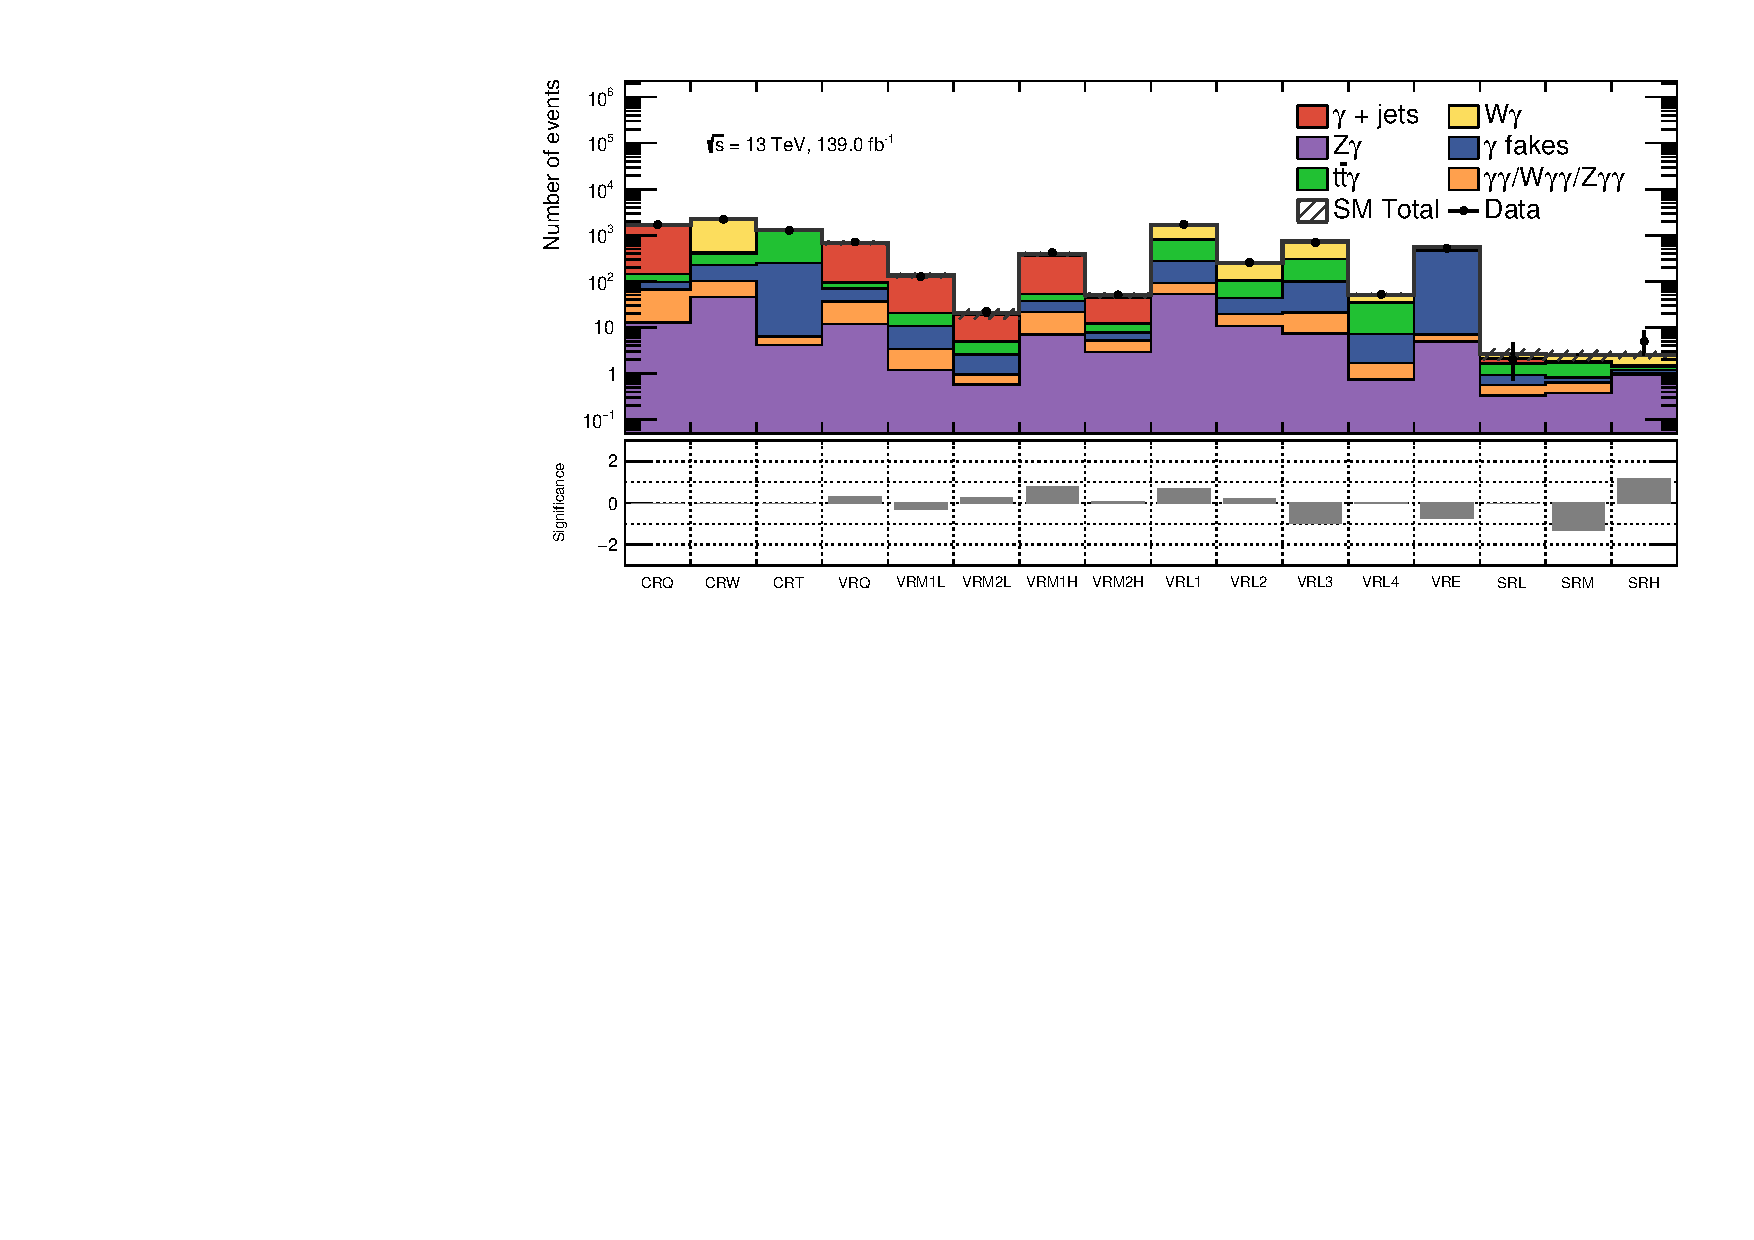
\includegraphics[width=0.89\textwidth]{images/results/fr2_unblind/regions_pull_significance.pdf}
  \caption{Resumen de la estimación de fondo y datos observados para cada región de control, validación y señal empleadas en el análisis. Abajo se muestra la diferencia entre el fondo estimado y los datos observados, en unidades de desviación estándar con respecto a la incerteza total del fondo.}
  \label{fig:regions_pulls_unblinded}
\end{figure}


\begin{figure}[!hb]
   \centering
   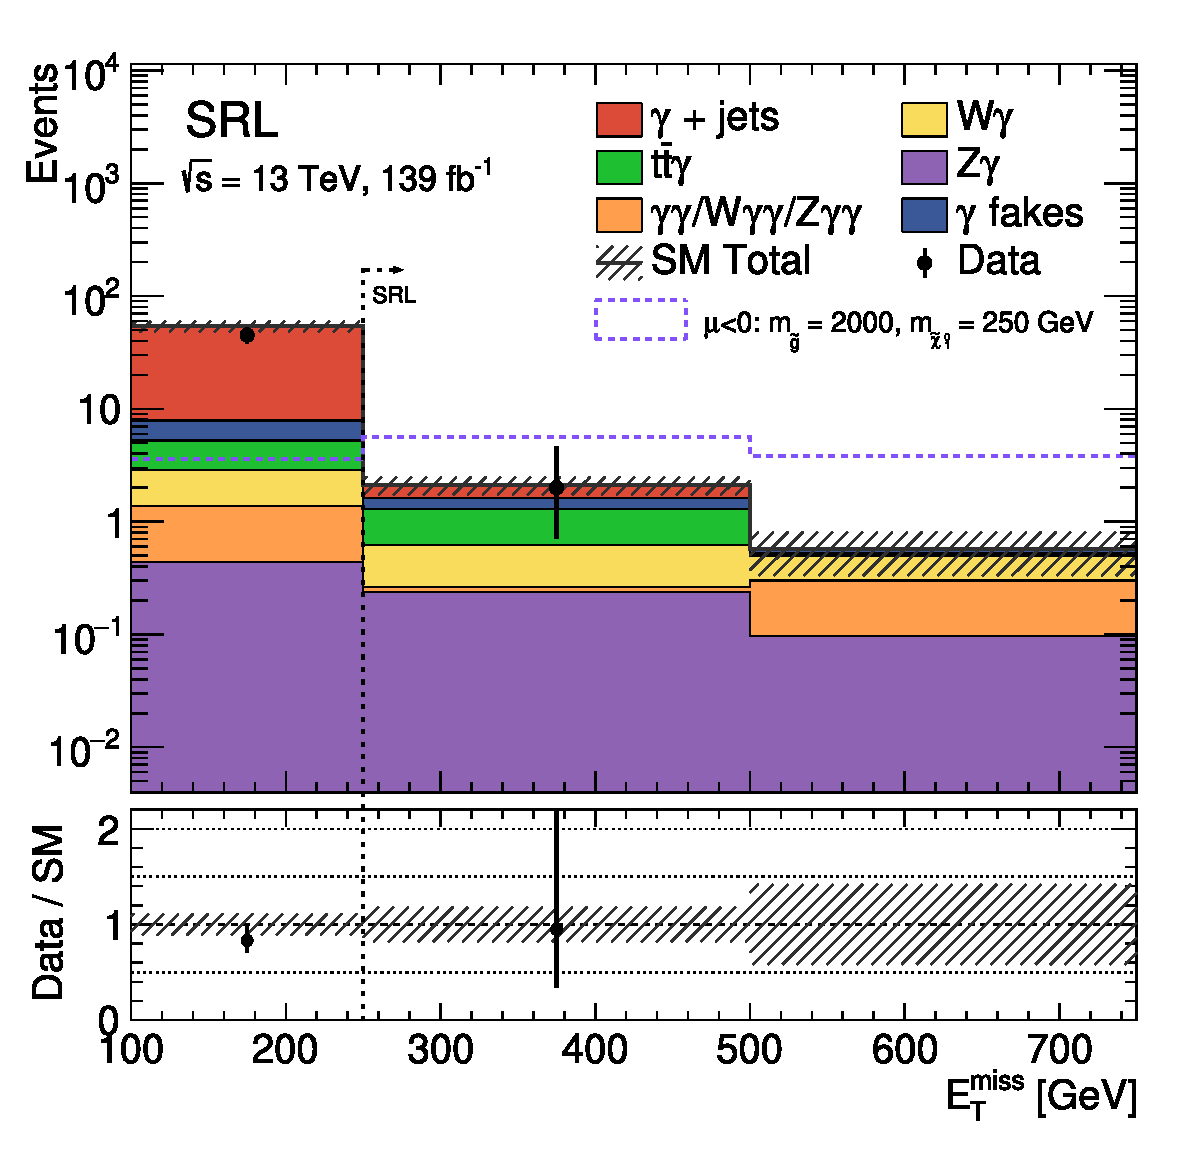
\includegraphics[width=0.48\textwidth]{images/results/fr2_unblind/sigReg_SRL_fr2_met_et_v2.pdf}
   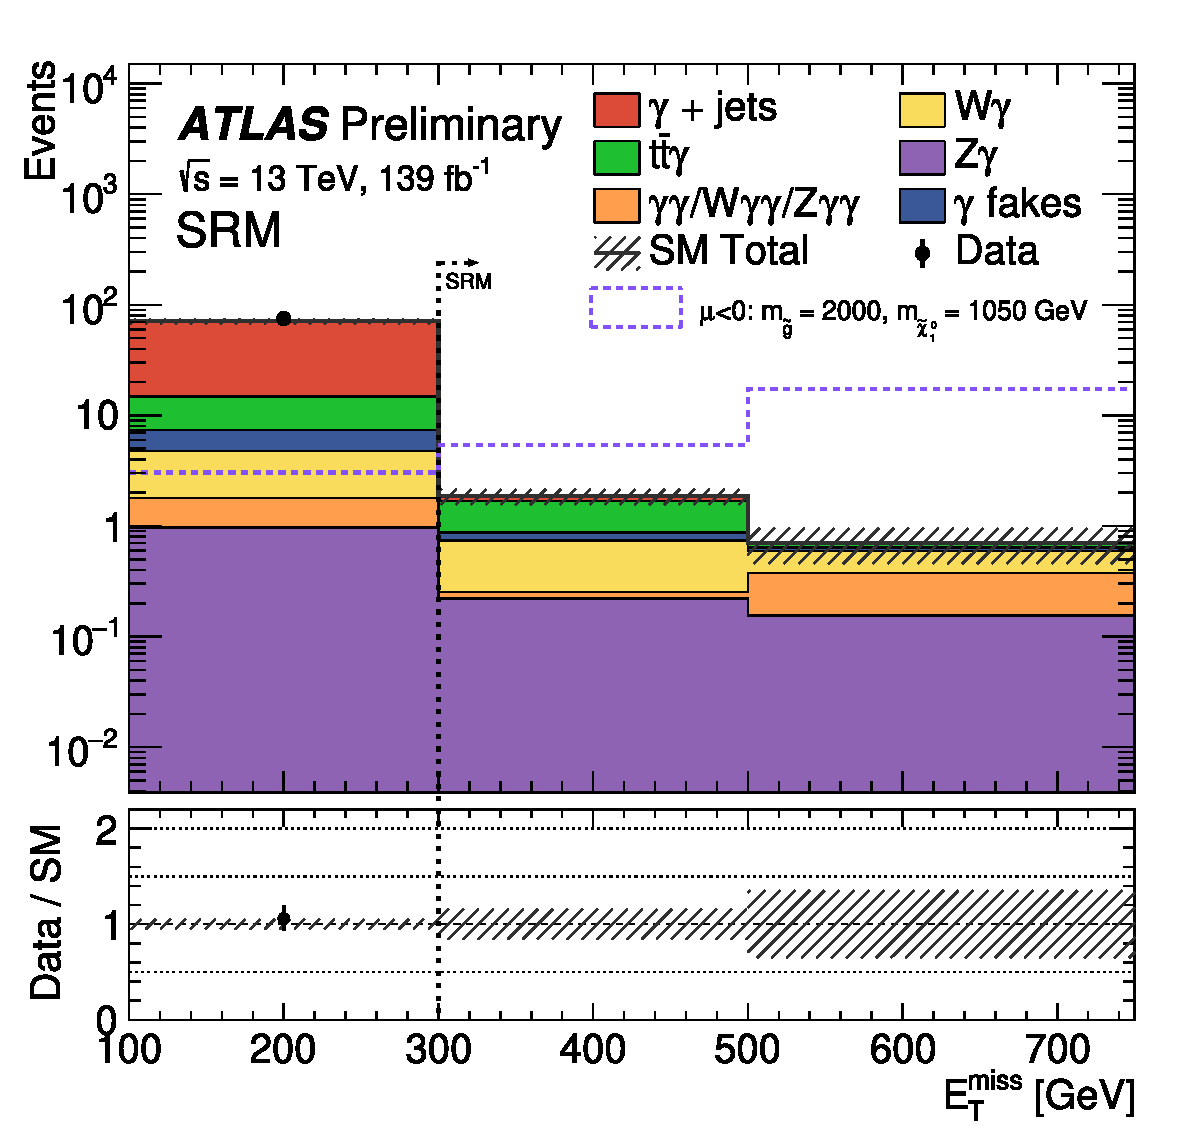
\includegraphics[width=0.48\textwidth]{images/results/fr2_unblind/sigReg_SRM_fr2_met_et_v2.pdf}
   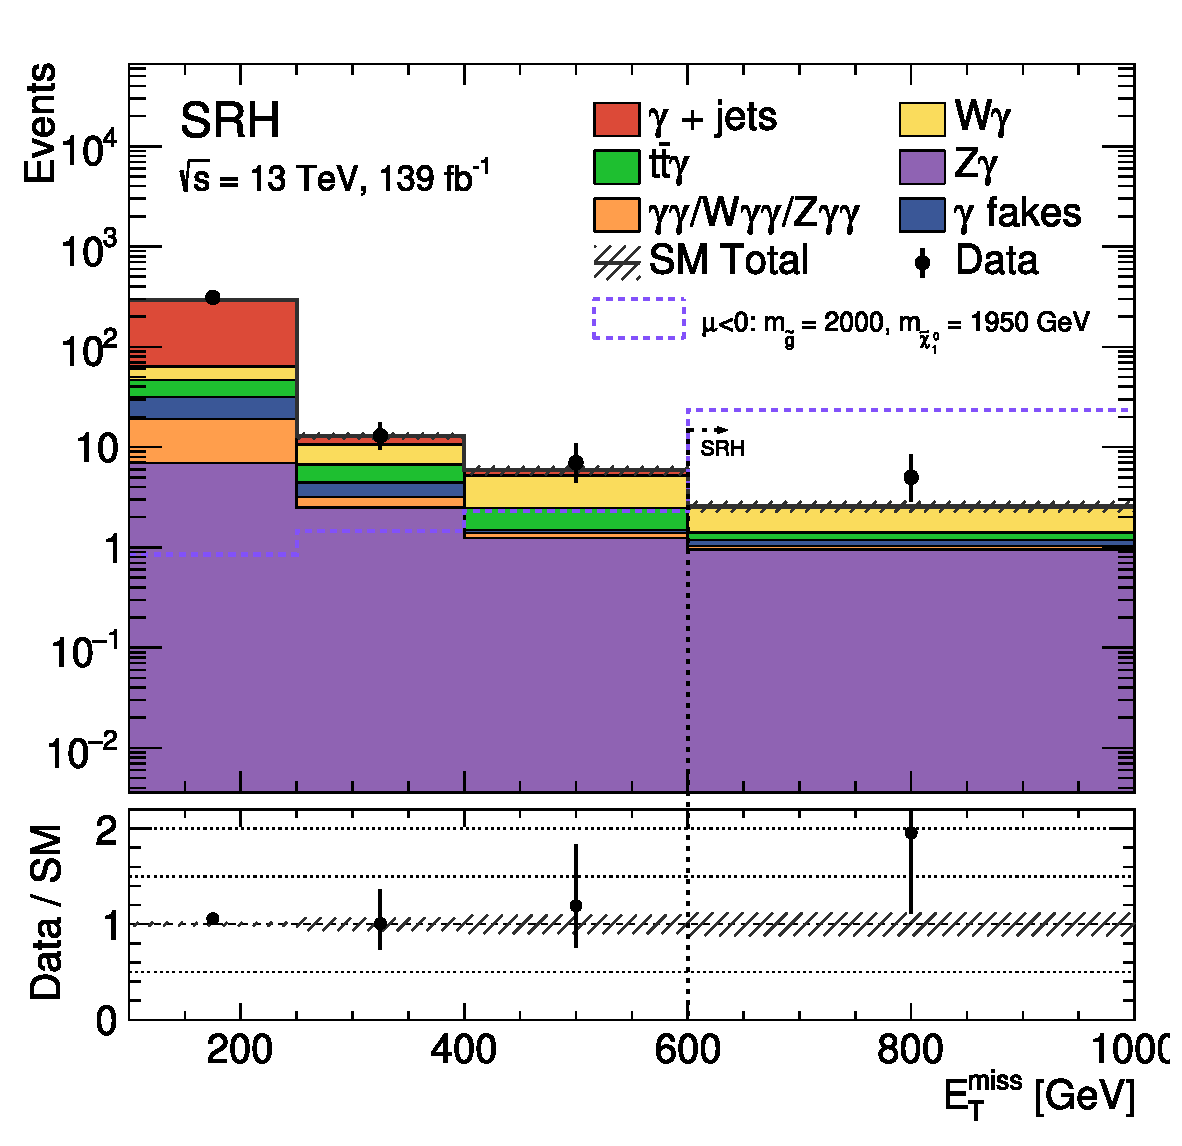
\includegraphics[width=0.48\textwidth]{images/results/fr2_unblind/sigReg_SRH_fr2_met_et_v2.pdf}
   \caption{Distribución de \met para los datos observados y la estimación de los fondos, en las regiones de señal SRL (izquierda), SRM (derecha) y SRH (abajo), omitiendo el corte en esa misma variable (N-1). Se incluye además la distribución del punto de señal más significativo para cada región.}
   \label{fig:met_n-1_SRL_SRM_SRH_fr2}
\end{figure}


% \solved{Falta la tabla de sistematicos} done

\begin{table}[ht!]
  \centering
  \caption{
  Resumen porcentual del aporte de las distintas incertezas sistemáticas en las regiones de señal, luego del ajuste de solo fondo. Debido a que las incertezas individuales pueden estar correlacionadas, la incerteza total no necesariamente es igual a la suma cuadrática de cada una.}
  %\resizebox{\textwidth}{!}{
    \begin{tabular}{lccc}
      \hline
      \hline
                                                  & SRL [\%] & SRM [\%] & SRH [\%] \\
      \hline
      \hline
      Incerteza total (estad.\ + sist.)           & 28       & 25       &  17  \\
      Incerteza estadística                    & 20       & 15       &  12  \\
      %Expected SM events & $2.67 \pm 0.54$ & $2.55 \pm 0.39$ & $2.55 \pm 0.31$ \\ %This uncertainty here is only statistical, because it was obtained without systematics.
      \hline
      Escala de energía y resolución de los jets             & 18       & 19       & 4.1  \\
      Calibración del $b$-tagging                       & 3.2     & 4.3     & 3.6  \\
      \textit{Jfakes}                                   & 2.1     & 2.5     & 2.3  \\
      Incertezas teóricas                                  & 3.6     & 3.1     & 10    \\
      \textit{Efakes}                              & 1.4     & 1.9     & $< 1$   \\
      Escala de energía y resolución de los electrones/fotones & 5.5     & 1.1     & 4.1  \\
      Reconstrucción e identificación de muones      & 2.6     & 1.8     & $< 1$   \\
      Identificación y aislamiento de fotones  & 2.6     & 2.1     & 1.1  \\
      Corrección por pile-up                         & $< 1$      & 1.2     & 1.0  \\
      Escala y resolución del término soft de \met & $< 1$      & $< 1$      & $< 1$   \\
      Luminosidad         & $< 1$      & $< 1$      & $< 1$   \\
      %                                             & SRL [\%] & SRM [\%] & SRH [\%] \\
      % \midrule
      % Total (stat. + syst.) uncertainty           & 28.0     & 24.9     &  17.4 \\
      % Statistical uncertainty                     & 20.2     & 15.3     &  12.2 \\
      % %Expected SM events & $2.67 \pm 0.54$ & $2.55 \pm 0.39$ & $2.55 \pm 0.31$ \\ %This uncertainty here is only statistical, because it was obtained without systematics.
      % \midrule
      % Jet energy scale and resolution             & 17.8    & 18.5    & 4.1  \\
      % b-tagging calibration                       & 3.2     & 4.3     & 3.6  \\
      % Jet fakes                                   & 2.1     & 2.5     & 2.3  \\
      % MC theory                                   & 3.6     & 3.1     & 10.2 \\
      % Electron fakes                              & 1.4     & 1.9     & < 1  \\
      % Electron/photon energy resolution and scale & 5.5     & 1.1     & 4.1  \\
      % Muon reconstruction and identification      & 2.6     & 1.8     & < 1  \\
      % Photon ID and isolation                     & 2.6     & 2.1     & 1.1  \\
      % Pile-up reweighting                         & < 1     & 1.2     & 1.0  \\
      % \MET\ soft-term scale and resolution        & < 1     & < 1     & < 1  \\
      \hline
      \hline
    \end{tabular}
  %}
\label{tab:syst_rel_impact}
\end{table}




\subsection{Límites independientes del modelo}


Dado el buen acuerdo entre la estimación del fondo y los datos observados en las distintas SRs, se establecen límites superiores en el número de eventos de cualquier fenómeno más allá del SM con el estado final del análisis. Los límites se establecen para cada SR con un nivel de confianza del 95\%, utilizando el estadístico de prueba definido en la Ecuación \ref{ec:st_qmu}, y las prescripciones para los $\text{CL}_{s}$ de la Ecuación \ref{eq:cls_limits}. Para ello se realiza un muestreo del número de eventos de señal para un cierto modelo, y se encuentra cuándo el valor de $\text{CL}_{s}$ cae por debajo del 5\%, método descripto en la Sección \ref{sec:flujo_busqueda}. La distribución de los distintos estadísticos de prueba se aproxima mediante la generación de {$\smallsim$}50000 toys.

En la Tabla \ref{tab:model_indep_ul} se muestran los límites superiores en el número de eventos en cada región de señal, tanto observados como esperados. Los límites observados son de $4.73$, $3$ y $7.55$ para las SRL, SRM y SRH respectivamente, lo que implica que cualquier modelo que prediga un número menor de eventos en dichas regiones, ya está excluido por el presente análisis. A su vez, se muestra el límite en la sección eficaz visible, obtenido a partir de dividir el anterior límite por la luminosidad total integrada, y multiplicarlo por la aceptancia (fracción de eventos que pasan todas las selecciones cinemáticas a nivel generador) y la eficiencia (fracción de esos eventos que pasan los cortes a nivel detector). 
Se incluye el p-value de descubrimiento, que para regiones donde la predicción supera lo observado, se fija a un valor de $0.5$. En la región SRH el p-value es de $0.09$, lo que implica que las observaciones son compatibles con la hipótesis de <<solo fondo>>.


\begin{table}[!h]
  \centering
  \caption{Límites superiores en el número de eventos con un nivel de confianza del 95\% para cada región de señal, tanto observados como esperados. Adicionalmente se muestran los límites equivalentes en la sección eficaz visible, junto con el p-value de descubrimiento. Este último limitado a $0.5$ cuando el número de eventos observados es menor al esperado.}

    \begin{tabular}{lccccc}
    %\begin{tabular}{l|c|c|ccccc}
      \hline
      \hline
      Signal Region  & $S_{\mathrm{obs}}^{95}$  & $S_{\mathrm{exp}}^{95}$ & $\langle\epsilon{\sigma}\rangle_{\mathrm{obs}}^{95}$ [fb]  & $\langle\epsilon{\sigma}\rangle_{\mathrm{exp}}^{95}$ [fb] & $p_{0}$ ($Z$)\\
      \hline
      \hline
      SRL     &   4.73   &   $4.7^{+2.2}_{-1.2}$ &  0.034   &   $0.034^{+0.016}_{-0.009}$    &    0.50 (0.00)  \\ 
      SRM    &   3       &   $4.6^{+1.8}_{-1.1}$ &  0.022   &   $0.033^{+0.013}_{-0.008}$     &    0.50 (0.00)  \\ 
      SRH     &   7.55   &   $4.8^{+1.9}_{-1.4}$ &  0.054   &   $0.035^{+0.014}_{-0.010}$    &    0.09 (1.32)  \\
      \hline
      \hline
    \end{tabular}
    \label{tab:model_indep_ul}
  \end{table}



\subsection{Límites dependientes del modelo}


Se establecen los límites dependientes del modelo, buscando aquellos puntos del modelo de señal para los cuales $\text{CL}_{s}=0.05$, como se describe en la Sección \ref{sec:flujo_busqueda}. Dichos límites son calculados de forma independiente para cada región de señal, y luego combinados en un límite total. Para ello se elige de cada punto de señal, la región con mejor límite esperado, y se emplea su $\text{CL}_{s}$ para realizar la interpolación. La misma se realiza mediante el módulo \texttt{Scipy} \cite{2020SciPy-NMeth}, empleando la interpolación \texttt{multiquadratic} con el parámetro \texttt{smooth} igual a $0.1$. La distribución de los distintos estadísticos de prueba se aproxima mediante la generación de {$\smallsim$}50000 toys.

En la Figura \ref{fig:limit_plot_combined} se muestran los límites observados y esperados, combinando los resultados de las tres regiones de señal, para los que se incluye la variación de las incertezas sistemáticas en $\pm1\sigma$. Para los límites esperados se varían las incertezas experimentales, mientras que para los observados la incerteza en el cálculo de la sección eficaz del modelo. Estos límites excluyen a 95\% de intervalo de confianza la producción de gluinos con masas de hasta aproximadamente $2300\ \gev$, para la mayoría de las masas de neutralino estudiadas. 


\begin{figure}[ht!]
  \centering

  %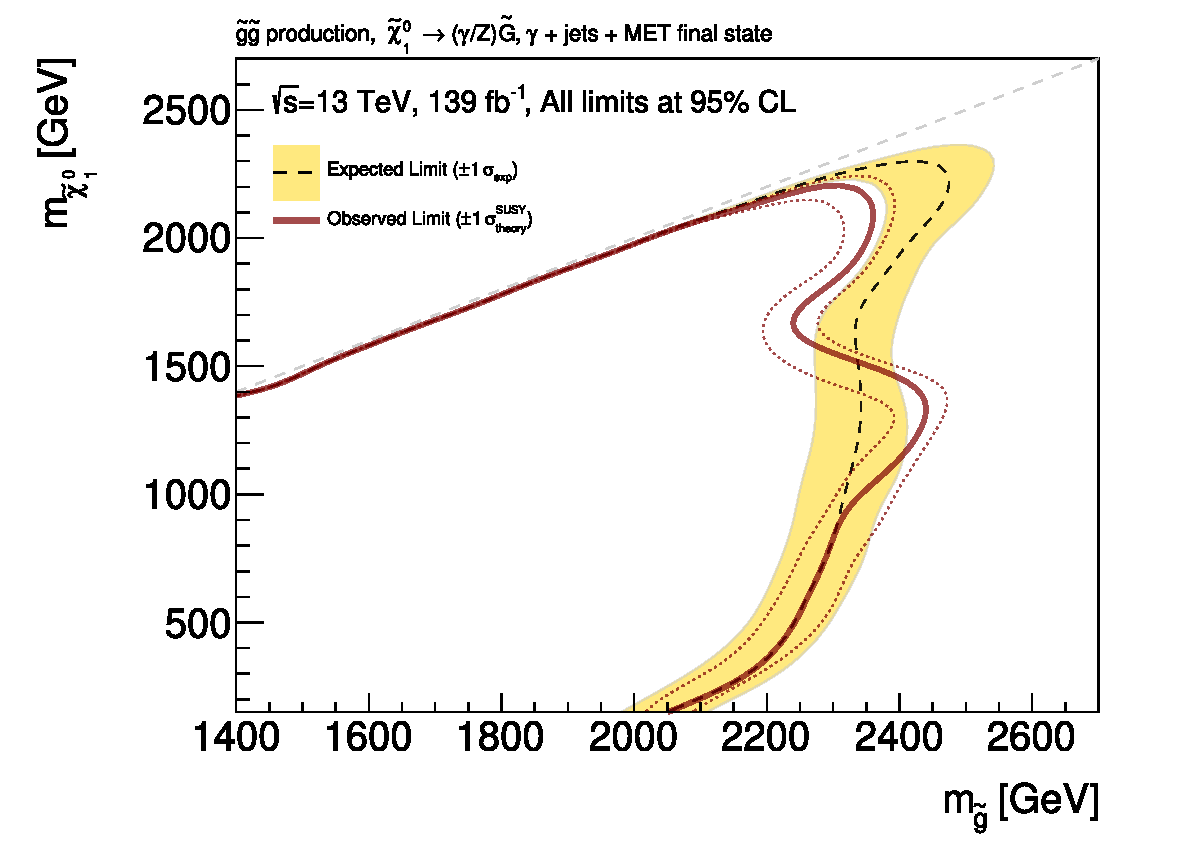
\includegraphics[width=0.45\textwidth]{figures/fr2_unblind/phjets_contour_plot_BestSR_wMatplotLib.pdf}
  % 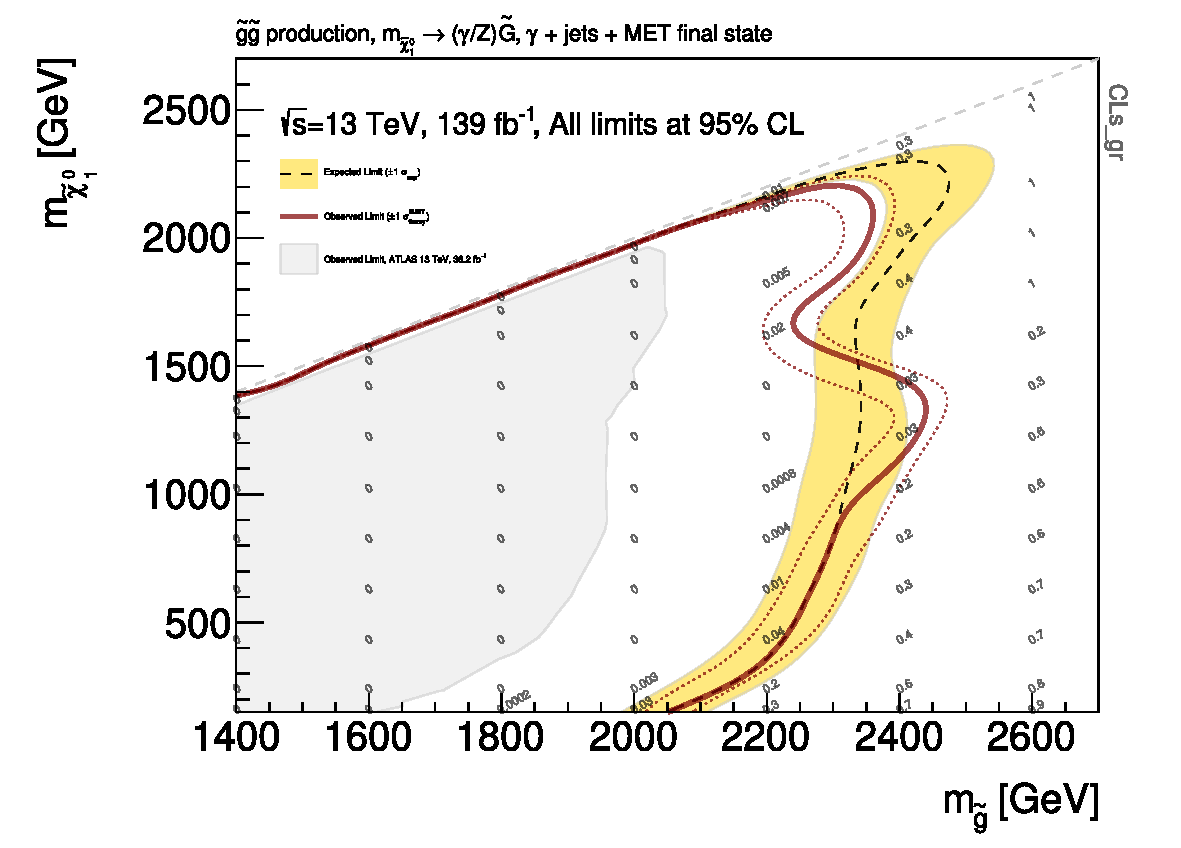
\includegraphics[width=0.45\textwidth]{figures/limits_plots/contour_plot_gZBestSR_wMatplotLib_full.pdf}
  %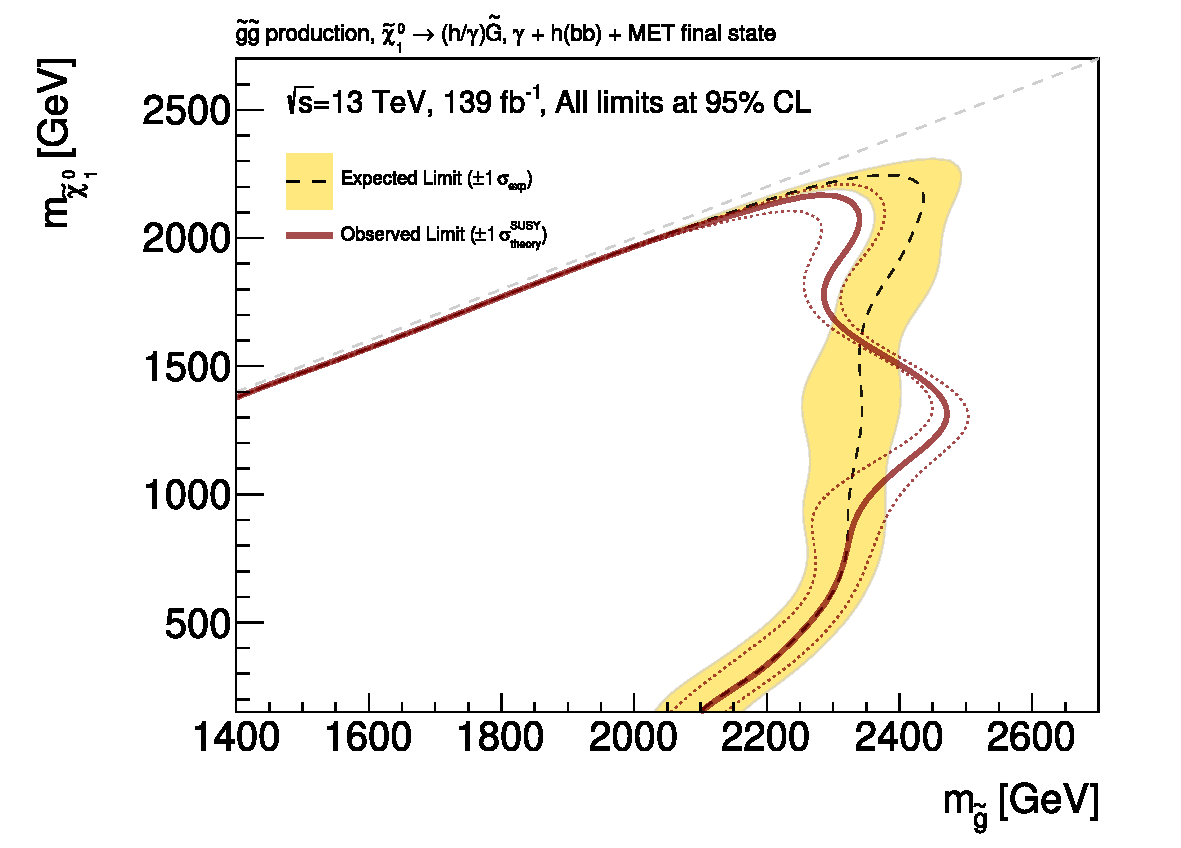
\includegraphics[width=0.45\textwidth]{figures/fr2_unblind/phb_contour_plot_BestSR_wMatplotLib.pdf}
  % 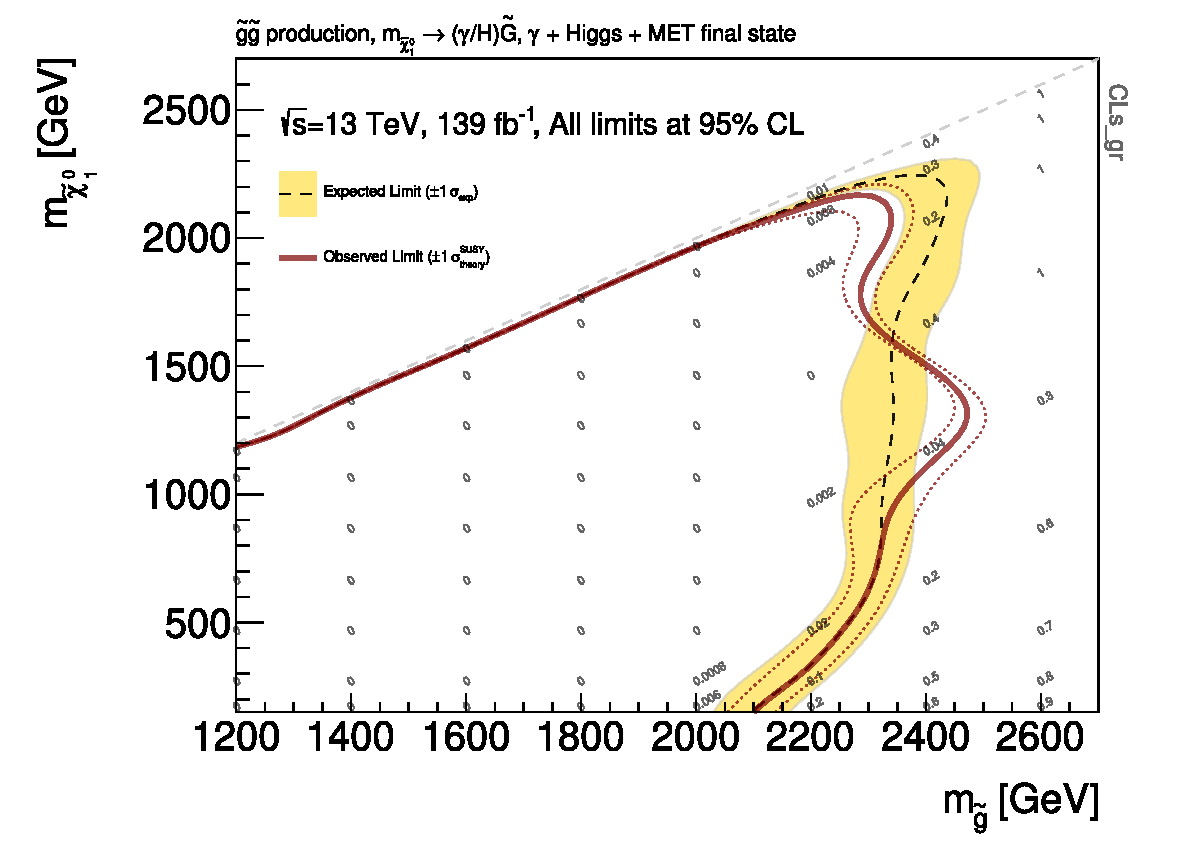
\includegraphics[width=0.45\textwidth]{figures/limits_plots/contour_plot_gHBestSR_wMatplotLib_full.pdf}

  \includegraphics[width=0.9\textwidth]{images/results/limits_plots/contour_plot_gHBestSR_wMatplotLib_full.pdf}

  \caption{Límites observados (línea roja) y esperados (línea negra punteada) para una luminosidad integrada de $139\ \ifb$ a 95\% de intervalo de confianza, combinando los resultados de las tres regiones de señal. Las incertezas en los límites se obtienen variando en $\pm1\sigma$ las incertezas experimentales y en la sección eficaz de los puntos de señal. Los números en gris muestran el $\text{CL}_{s}$ para cada punto de señal.}
  \label{fig:limit_plot_combined}

\end{figure}





